\documentclass[runningheads,14pt,a4paper,openany]{book}

% Добавя възможност за сензитивни хипер-връзки в самия документ.
\usepackage[pdftex, bookmarks, linktocpage]{hyperref}
% Команда с множество опции за настройка на поведението на пакета hyperref, с най-полезната опция - кирилизация на заглавията от Bookmarks в Acrobat.
\hypersetup{unicode=true, colorlinks=true, linkcolor=black, citecolor=black, urlcolor=black}
\usepackage{nameref}
\usepackage[utf8x]{inputenc}
% Използва се за цвят на заглавните редове в таблиците.
\usepackage[table]{xcolor}
\usepackage[english,bulgarian]{babel}
\usepackage{shorttoc}
\usepackage[pdftex]{graphicx}
\usepackage{imakeidx}
\usepackage{placeins}
% Използва се за включване на кориците под формата на PDF файлове.
\usepackage{pdfpages}
% Служи за управление на заглавията.
\usepackage{fancyhdr}
\usepackage{listings}
% Служи за списък на формулите.
\usepackage{tocloft}
\usepackage{amsmath,amssymb,amsthm}

% Добавени от доц. Вера Ангелова.
%\usepackage{longtable}
%\usepackage{pifont}   
%\usepackage{epsfig}
%\usepackage{etoc}
%\usepackage{wasysym}
%\usepackage{eurosym}
%\usepackage{slashbox}
%\usepackage{soul}
%\usepackage{enumitem}
%\usepackage{mathcomp}
%\usepackage{epstopdf}
%\usepackage{latexsym}
%\usepackage{eucal}
%\usepackage{mathrsfs}

% Директория в която се намират изображенията.
\graphicspath{{images/}}

\textheight 22.8cm
\textwidth 17cm
\oddsidemargin -0.54cm
\evensidemargin -0.54cm
\topmargin 1.5cm

\parskip=0.2cm
\parindent=20pt
\flushbottom

% Добавя черти под хедъра и над футъра.

\selectlanguage{bulgarian}

% Оформление на хедъра и футъра.
\lhead[\thepage \quad Тодор Балабанов, Зорница Атанасова, Румен Кетипов \quad \hfill]{}
\rhead[]{\hfill Статистическа обработка на данни с R \quad \thepage }
\cfoot[\em Лекции по компютърни науки и технологии на ИИКТ - БАН, № *, 20**]{\em Лекции по компютърни науки и технологии на ИИКТ - БАН, № *, 20**} 
\renewcommand{\headrulewidth}{1pt}
\renewcommand{\footrulewidth}{1pt}

\onecolumn
\makeindex[columns=2, title=Азбучен указател, intoc]

% Подменя думата използван а за ноемрация на фрагментите програмен код.
\renewcommand{\lstlistingname}{Листинг}

% Определя характеристиките на листигните за програмния код.
\lstset{backgroundcolor=\color{gray!30}, breaklines=true, language=r, frame=single}

\begin{document}

\def\ql{\textquotedblleft}\def\qr{\textquotedblright}


\includepdf[pages={1,2}]{images/front}
\thispagestyle{empty}

\voffset =-1truecm

% Използва се за номерация на страниците.
\renewcommand{\thepage}{\roman{page}}

% Смяна на названието за списъка от листингите.
\renewcommand{\lstlistlistingname}{Списък на листингите}

% Смяна на названието за списъка от формули.
\newcommand{\listequationsname}{Списък на формулите}
\newlistof{listofequations}{equ}{\listequationsname}
\newcommand{\listofequations}[1] {
	\addcontentsline{equ}{listofequations}{\protect\numberline{\theequation}#1}\par
}

\setcounter{page}{-1}
\thispagestyle{empty}
\pagestyle{empty}
\thispagestyle{empty}

% Тук стои таблицата със съдържанието, което се генерира от названието на главите.
\newpage
\thispagestyle{empty}
\pagestyle{empty}
\shorttoc{Теми}{0}
\thispagestyle{empty}
\pagestyle{empty}

% Тук стои таблицата със съдържанието, което се генерира от названието на главите и названието на секциите в тях.
\newpage
\thispagestyle{empty}
\pagestyle{empty}
\thispagestyle{empty}
\tableofcontents
\thispagestyle{empty}
\pagestyle{empty}

% Списък с фигурите.
\newpage
\listoffigures
\addcontentsline{toc}{chapter}{Списък на фигурите}

% Списък с листингите.
\newpage
\lstlistoflistings
\addcontentsline{toc}{chapter}{Списък на листингите}

% Списък с формулите. 
\newpage
%\listofequations
\addcontentsline{toc}{chapter}{Списък на формулите}

% Списък с таблиците. 
\newpage
\listoftables
\addcontentsline{toc}{chapter}{Списък на таблиците}

\pagestyle{fancy}
\newpage
\addcontentsline{toc}{chapter}{Предговор}
\chapter*{Предговор}
\pagenumbering{arabic}
\setcounter{page}{1}
\pagestyle{fancyplain}

Това учебно помагало е предвидено за студенти и докторанти, които в своите магистърски или докторски тези се сблъскват с потребността да извършат определени експерименти, а след това статистически да обработят получените резултати.

В съвременния живот нуждата от обработка на информация постоянно нараства. Налага се да бъдат вземани решения в множество ситуации от ежедневието ни. От своя страна, всяко решение е толкова по-успешно, колкото по-информирано е взето то. Статистическата обработка на събраната информация е една от основите за вземането на информирани решения. В областта на статистическата обработка съществуват множество софтуерни решения, като се започне от по-достъпните за хора без опит, като Microsoft Excel и се стигне до професионалните пакети, като SPSS, Matlab и Mathematica.

Настоящото учебното пособие представя програмния продукт R, който първоначално се разработва от Robert Gentleman и Ross Ihaka в University of Auckland през 1993 година. R е замислен като алтернатива на програмния продукт S, създаден от John Chambers, служител в Bell Labs. Първоначалният замисъл за R е да представлява инструмент, който да се използва в интерактивен режим, през командния ред. В последствие тази идея прераства в самостоятелен програмен език. Основното предназначение на R е обработка на данни, което включва въвеждане, пресмятане, визуализация на графики и отчети.

Езикът получава значително по-голяма популярност след 2000 година, като излиза от рамките на академичните среди и навлиза във финансовите среди, маркетинга, фармацията, социологията, психологията и в много други области. Най-често потребителите на R са хора с опит в програмни езици, като C/C++, Java, C\# или пък преди това са използвали други статистически пакети, като SAS, SPSS или дори Excel. Тези потребители дават значителен тласък в развитието на пакета R, добавяйки множество софтуерни приставки (add-ons).

В някои случаи R се оказва стряскащ и дори смущаващ, особено за начинаещите потребители, но с времето и с процеса по навлизане в материята овладяването му се улеснява и ускорява. Целта на това учебно помагало е да представи информацията по един достъпен и олекотен за възприемане начин. Изложени са предимно най-важните аспекти от използването на пакета R, което от своя страна дава стабилна основа за бъдещо самостоятелно развитие на читателя. Материалът е съобразен със съдържанието на курса „Анализ на данни с R“, провеждан в „Център за обучение“ към „Българска академия на науките. Учебното помагало е организирано в следните глави:

Глава 1 - \nameref{chapter01}: Представя процеса по изтегляне, инсталиране и стартиране на програмния продукт.

Глава 2 - \nameref{chapter02}: Разяснява основните концепции за работата с програмния продукт R, като акцентите са върху пакетната организация на продукта и как най-ефективно да бъдат използвани възможностите му. Разглеждат се базовите типове данни и основните математически операции. 

Глава 3 - \nameref{chapter03}: Демонстрира използването на функции в R. Разглеждат се също сложни типове данни, като вектори, фактори, извадки от данни, масиви и матрици. 

Глава 4 - \nameref{chapter04}: Представя възможностите на системата за въвеждане на данни от външни източници, чрез прочитане на файлове или ресурси в Глобалната мрежа. Също така, демонстрират се основните възможности на програмния продукт за визуализиране на данни и получени резултати.  



\newpage
\chapter{Инсталация и стартиране}
\label{chapter01}

Тъй като програмният продукт R се разработва под формата на софтуер с отворен код\index{отворен код}, то употребата му с нетърговска цел не изисква заплащане. За работа с R е достатъчно да се инсталира основният пакет, въпреки това съществува и интегрирана среда за разработка наречена R Studio. За нуждите на учебното помагало ще бъде използван само основният пакет. Всеки желаещ да разшири уменията си с използването на интегрираната среда за разработка, би могъл самостоятелно да разучи възможностите ѝ.

\section{Изтегляне на инсталационните файлове}

\begin{figure}[h!]
  \centering
  
\includegraphics[width=1.0\linewidth]{pic0001}
  \caption{Начална уеб страница на продукта}
\label{figure0001}
\end{figure}
\FloatBarrier

Както множество софтуерни продукти и R е достъпен за изтегляне\index{изтегляне на инсталатор} от уеб страницата на продукта в Интернет (Фиг. \ref{figure0001}) с адрес: http://www.r-project.org/

\begin{figure}[h]
  \centering
  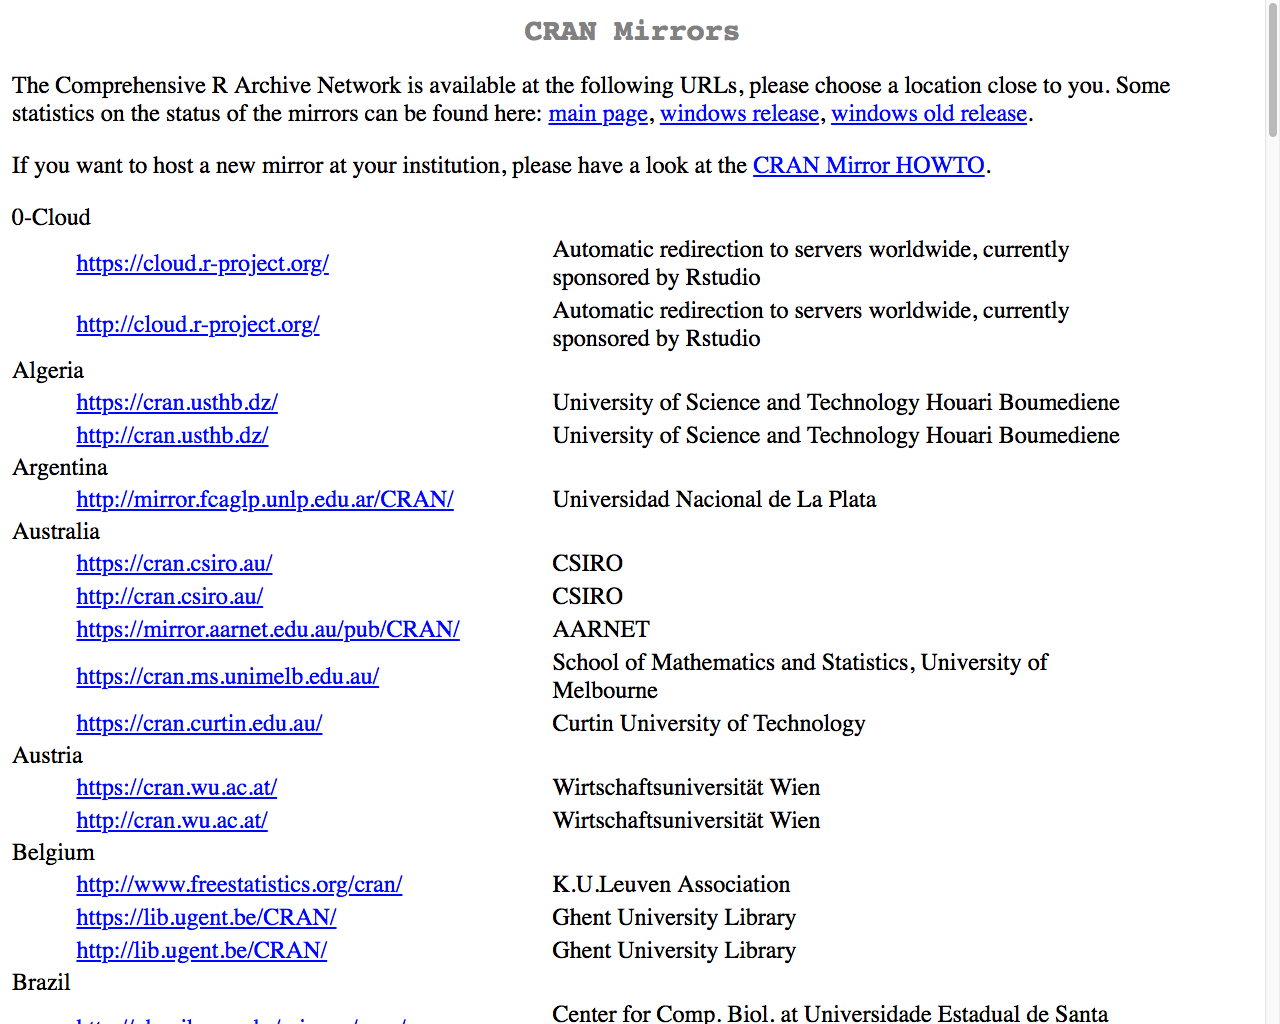
\includegraphics[width=1.0\linewidth]{pic0002}
  \caption{Списък със сървъри за изтегляне}
\label{figure0002}
\end{figure}
\FloatBarrier

В раздела за изтегляне са посочени множество активни връзки към различни географски локации (Фиг. \ref{figure0002}). Обичайна практика, при софтуерните продукти с отворен код, е наличието на множество сървъри, разположени по цял свят, да предлагат изтегляне на файловете нужни за инсталацията. Тази практика се е наложила най-вече за ускоряване на изтеглянето, също така и за намаляване на натоварването, което сървърите понасят при множество заявки. Не на последно място, много често за разпространението на инсталационните файлове се разчита на доброволческа информационна инфраструктура, за която не се заплаща.

\begin{figure}[h]
  \centering
  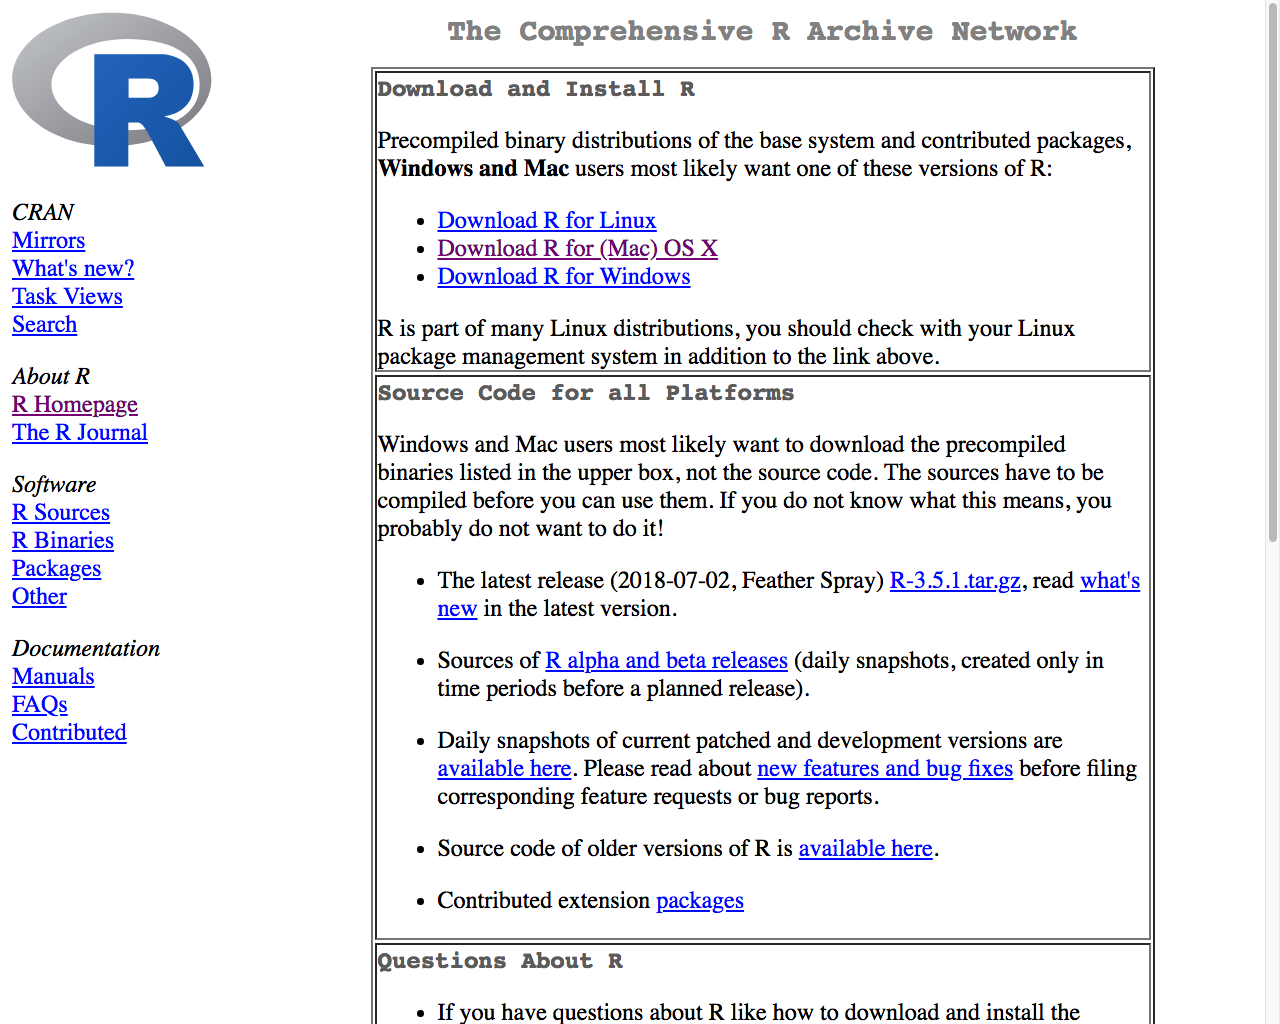
\includegraphics[width=1.0\linewidth]{pic0003}
  \caption{Избор на подходяща инсталация за операционната система }
\label{figure0003}
\end{figure}
\FloatBarrier

Често срещана практика е продуктите с отворен кода да се разпространяват за трите най-популярни операционни системи, този принцип е спазен и за продукта R (Фиг. \ref{figure0003}). При комерсиалните софтуерни продукти много често се залага на една единствена операционна система, но при продуктите с отворен код идеологията е, че трябва да се достигне до възможно най-голям брой потребители и поради тази причина се полагат допълнителни усилия софтуерът да работи на възможно най-много платформи (платформа – комбинация между хардуер и операционна система). Тази стратегия за дълготрайно развитие залага и на следващата особеност в развитието на продуктите с отворен код, а именно, че една част от потребителите с времето се превръщат в хора добавящи програмен код към продуктите. Освен вида на операционната система, от значение е и размерът на машинната дума, която процесорът поддържа. Към настоящия момент, най-разпространени са изчислителните машини с 64 битова машинна дума, но тъй като все още има много техника, която работи на 32 битова машинна дума, продуктът R е достъпен и за двата варианта.

\begin{figure}[h]
  \centering
  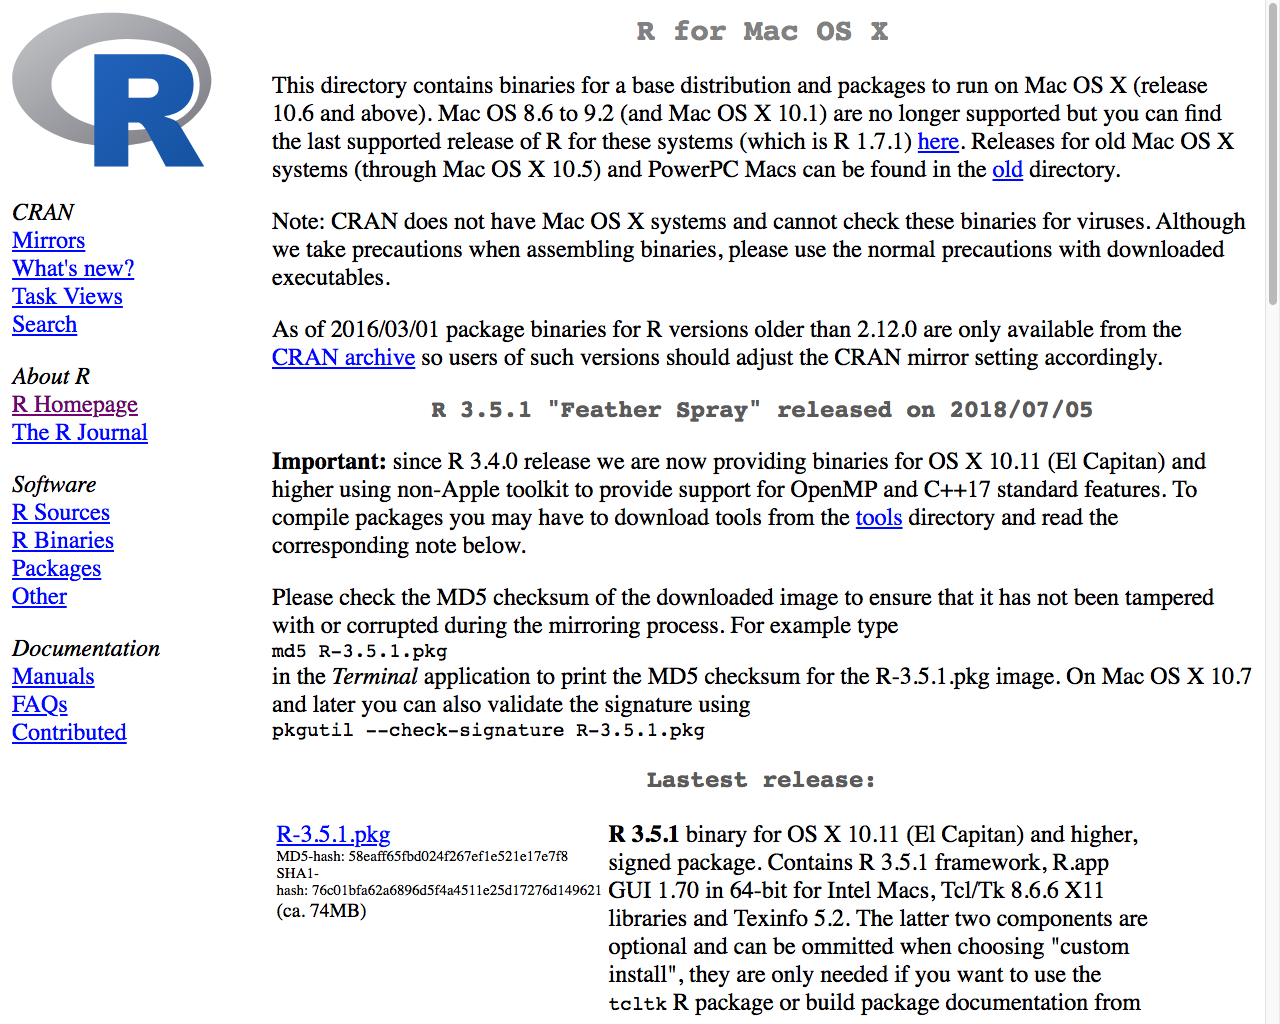
\includegraphics[width=1.0\linewidth]{pic0004}
  \caption{Избор на версия за изтегляне}
\label{figure0004}
\end{figure}
\FloatBarrier

Добра практика е при работата със софтуерни продукти, които се разпространяват като отворен код, винаги да се използва най-новата стабилна версия. В случая, за операционната система Mac OS X, това е версията 3.5.1, която е налична под формата на инсталационен файл R-3.5.1.pkg (Фиг. \ref{figure0004}).

\begin{figure}[h]
  \centering
  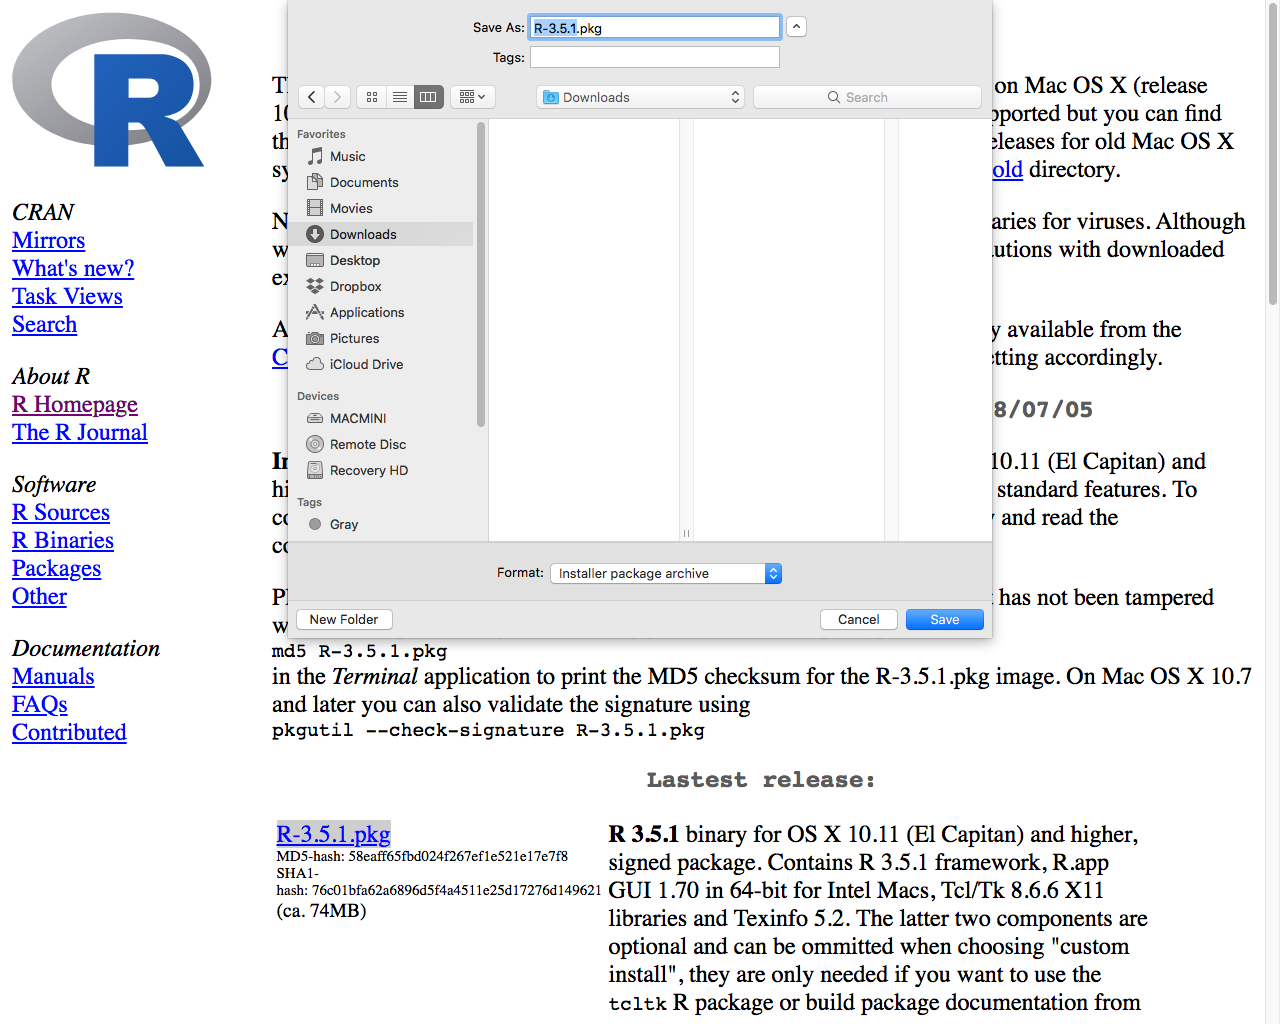
\includegraphics[width=1.0\linewidth]{pic0005}
  \caption{Запазване на инсталационния файл}
\label{figure0005}
\end{figure}
\FloatBarrier

\section{Инсталация}

За всяка от операционните системи е достатъчно потребителят да следва инструкциите и инсталацията\index{инсталация на продукта} протича безпроблемно по указаните стъпки. 

\begin{figure}[h]
  \centering
  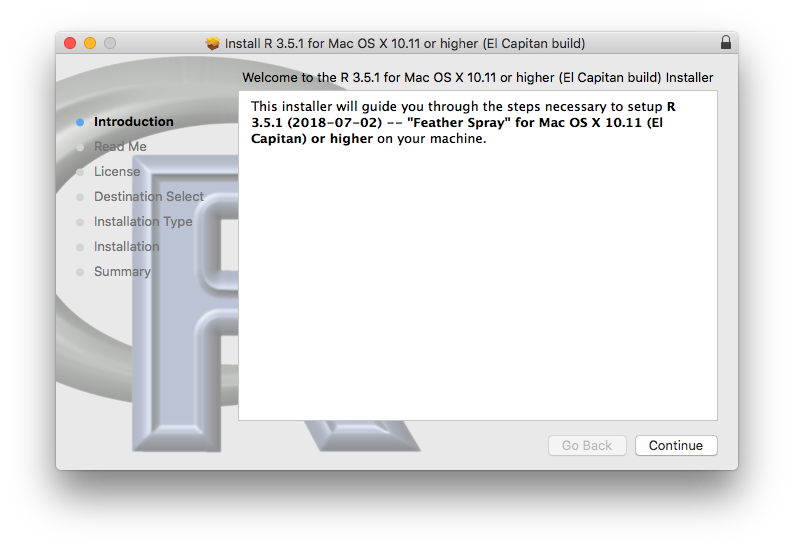
\includegraphics[width=1.0\linewidth]{pic0006}
  \caption{Активиране на инсталатора}
\label{figure0006}
\end{figure}
\FloatBarrier

С двойно кликване на мишката се активира инсталаторът (Фиг. \ref{figure0006}). След което следва екран с подробности за самата инсталация (Фиг. \ref{figure0007}).

\begin{figure}[h]
  \centering
  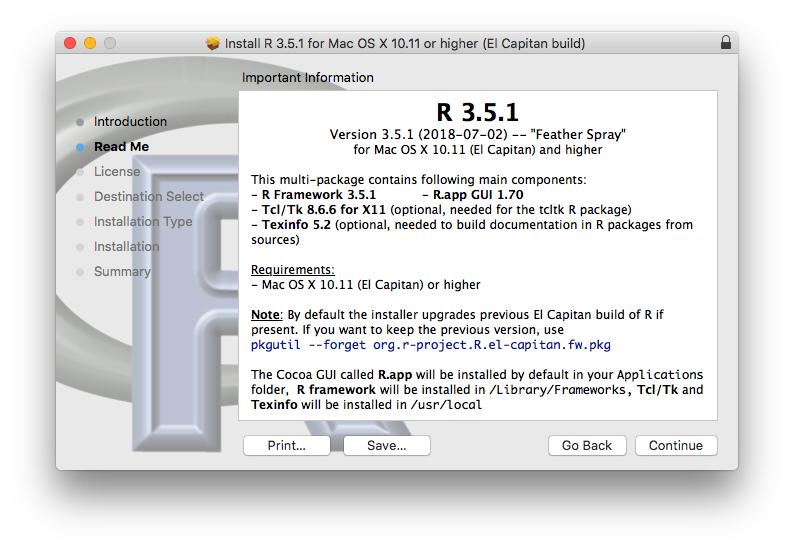
\includegraphics[width=1.0\linewidth]{pic0007}
  \caption{Подробности за инсталацията}
\label{figure0007}
\end{figure}
\FloatBarrier

От съществено значение е потребителите на продукти с отворен код да са добре запознати с условията, при които те получават продуктите, особено когато е без заплащане. Поради тази причина, потребителят трябва изрично да се съгласи с условията на лиценза, под който се разпространява продуктът R (Фиг. \ref{figure0008}, \ref{figure0009}).

\begin{figure}[h]
  \centering
  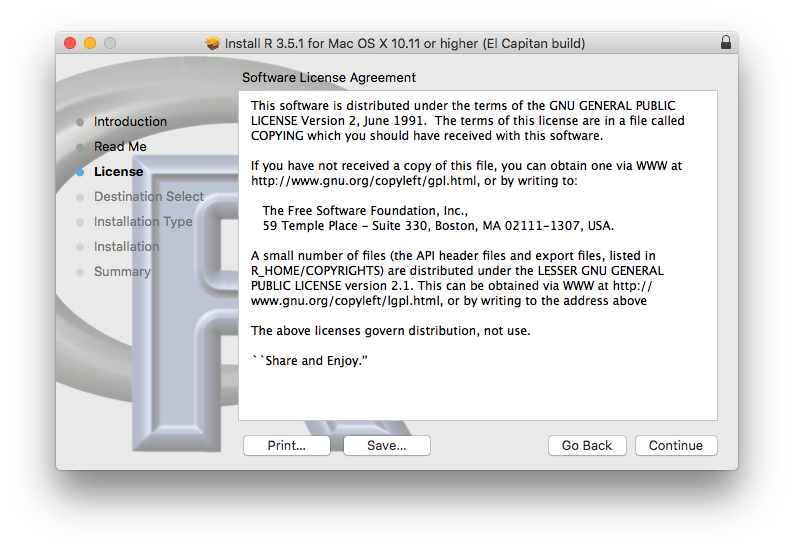
\includegraphics[width=1.0\linewidth]{pic0008}
  \caption{Лицензно споразумение за ползване}
\label{figure0008}
\end{figure}
\FloatBarrier

Софтуерният продукт R се разпространява под отворен лиценз GPL2, който в най-общи линии очертава рамките на условията, при които потребителите получават софтуера. Най-важните клаузи в лиценза са свързани с липса на гаранция и с изричното съгласие на потребителя, че производителят не носи никаква юридическа отговорност, произтекла от употребата на софтуерния продукт. Пълният текст на лиценза\index{софтуерен лиценз} е достъпен в уеб страницата на фондацията, която го поддържа \cite{gpl2}.

\begin{figure}[h]
  \centering
  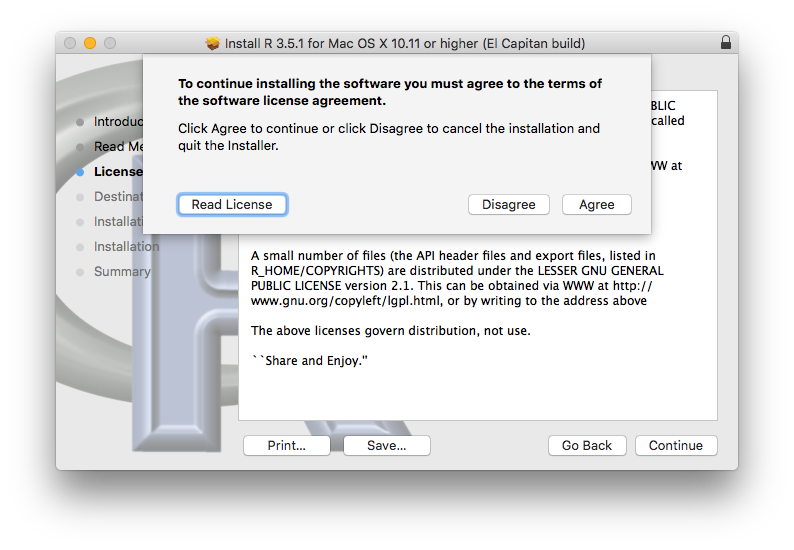
\includegraphics[width=1.0\linewidth]{pic0009}
  \caption{Изрично съгласие}
\label{figure0009}
\end{figure}
\FloatBarrier

Съвременните операционни системи са от отворен тип и инсталациите на допълнителни софтуерни продукти се явяват своеобразно разширение на операционната система. Поради тази причина, всеки създател на операционна система е избрал правила и начини за добавяне на софтуерни продукти. Една от основните характеристики е определяне на директория във файловата система на операционната система, където новодобавеният софтуер да бъде поставен. Някои операционни системи (например Linux базираните дистрибуции) използват специално организиран мениджър на пакетите, който има грижата за консистентността на добавяните софтуерни продукти. При Mac OS X също е налична възможността за автоматично управление на инсталациите, но е дадена и възможност потребителят да избира мястото на инсталация. В операционната система Microsoft Windows, потребителят решава къде да помести новоинсталирания софтуер.

\begin{figure}[h]
  \centering
  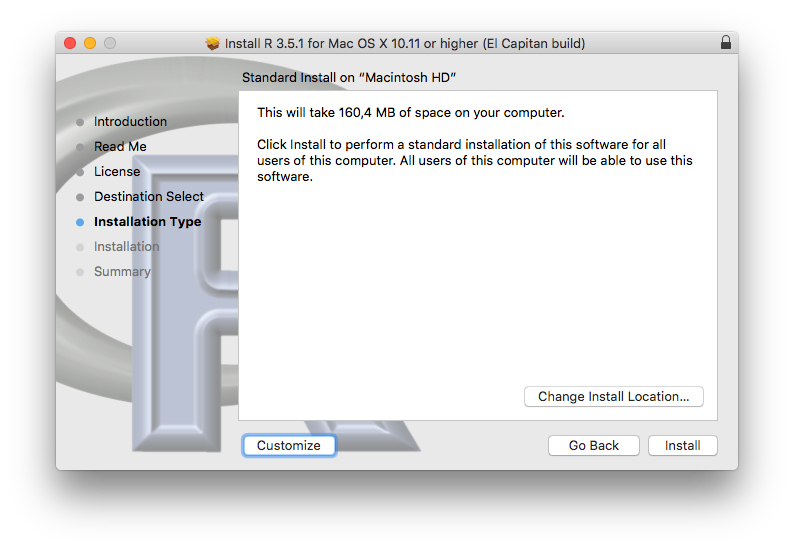
\includegraphics[width=1.0\linewidth]{pic0010}
  \caption{Информация за директорията и използваното дисково пространство}
\label{figure0010}
\end{figure}
\FloatBarrier

При желание е възможно да бъде подменена инсталационната директория (Фиг. \ref{figure0010}).

\begin{figure}[h]
  \centering
  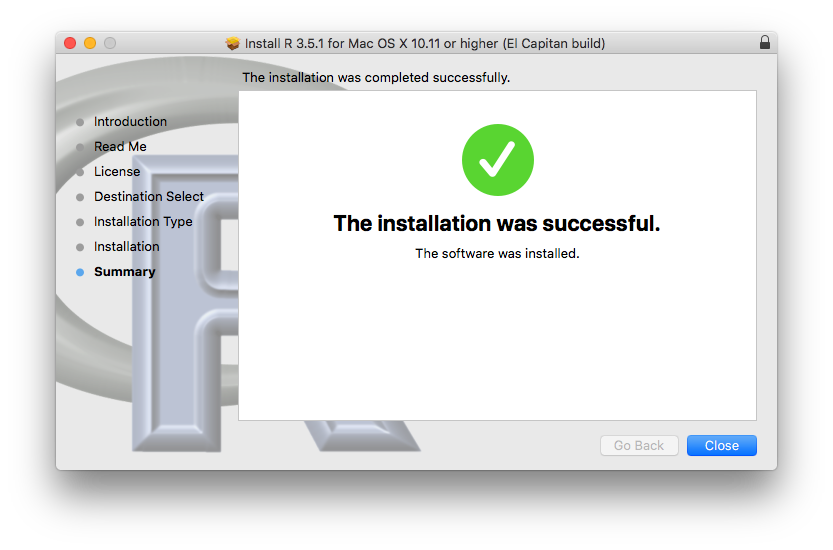
\includegraphics[width=1.0\linewidth]{pic0011}
  \caption{Успешно приключване на инсталацията}
\label{figure0011}
\end{figure}
\FloatBarrier

Инсталацията приключва със съобщение за успешно изпълнение (Фиг. \ref{figure0011}).

\section{Работа в режим на команди}

Инсталаторът създава икона за стартиране на R командния интерпретатор.

\begin{figure}[h]
  \centering
  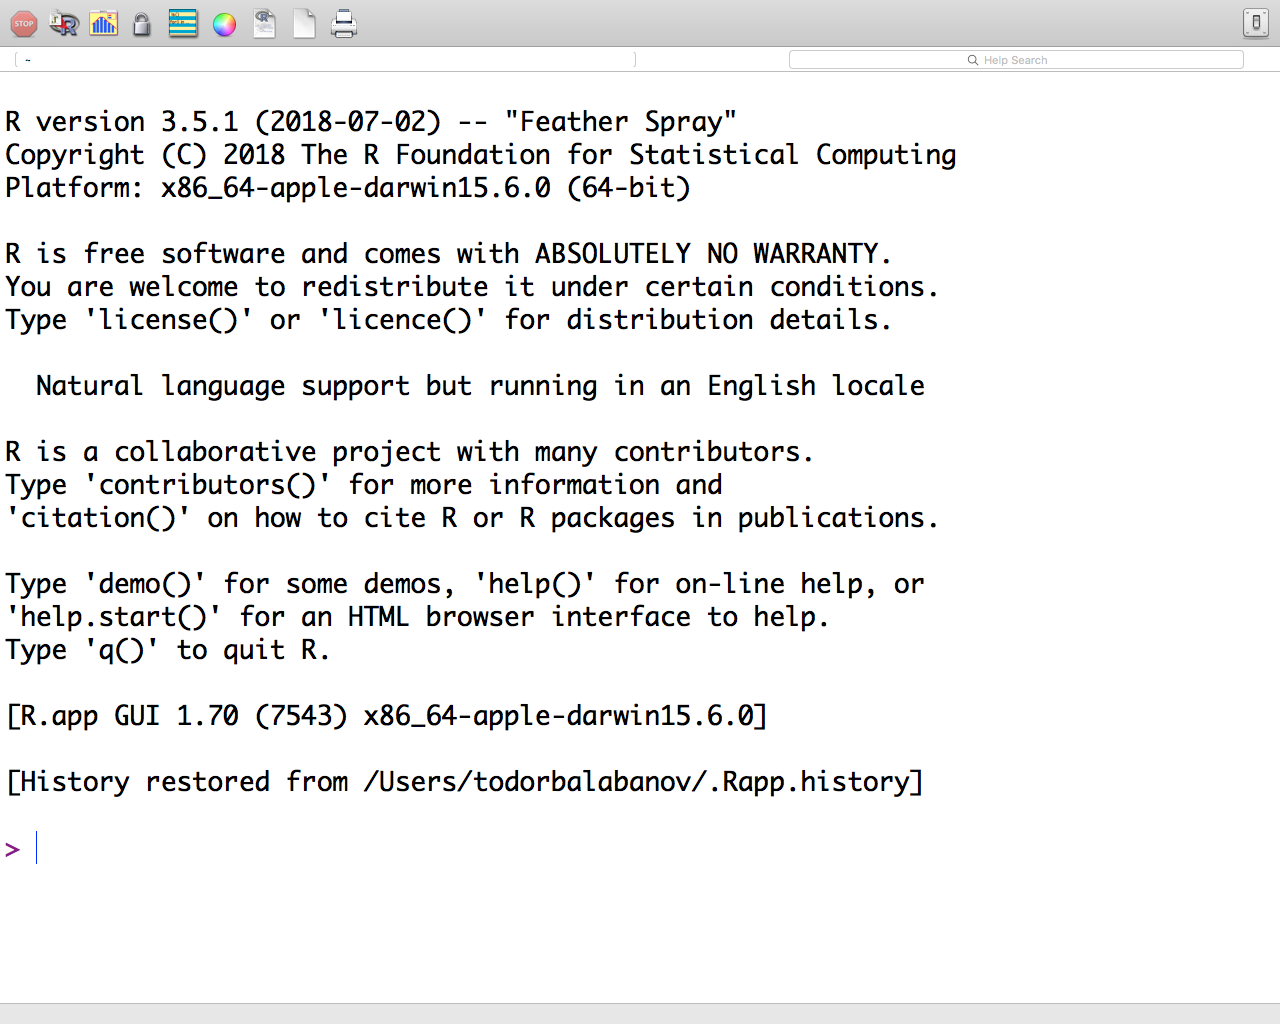
\includegraphics[width=1.0\linewidth]{pic0012}
  \caption{Основен прозорец на продукта}
\label{figure0012}
\end{figure}
\FloatBarrier

При успешна инсталация и стартиране, потребителят получава достъп до прозорец, служещ като команден интерпретатор\index{команден интерпретатор} (Фиг. \ref{figure0012}). Първоначалният замисъл за продукта R е бил това да представлява интерпретатор на команди. В интерактивен режим потребителят въвежда команда и наблюдава получения резултат. Макар и това да е основният начин за работа, R позволява последователността от команди да бъде записана във файл и да се изпълняват като единен скрипт. За много потребители, особено такива с предишен опит в софтуерни продукти със силно застъпен графичен потребителски интерфейс (например статистически анализ на данни в Microsoft Excel), използването на терминал с команди първоначално е трудно и дори дразнещо, но с напредване на времето потребителите оценяват гъвкавостта, която този начин на работа позволява. Използването на поредица от команди често се оказва значително по-бърз начин за работа, в сравнение с подготовката на експеримент в софтуер с графичен интерфейс. Също така, наличието на серията команди дава възможност значително по-бързо експериментът да бъде преповторен. Често при по-голям обем данни софтуерните пакети с графичен потребителски интерфейс забавят работата си неприемливо много. И не на последно място, наличието на статистическият модел като скрипт позволява използването на системи за контрол на версиите (каквато примерно е Git и облачната услуга GitHub), нещо което търговските бинарни файлови формати (например XLSX, в Microsoft Excel) не позволяват. При работата с командния интерпретатор на R, клавишът „стрелка нагоре“ повтаря последната използвана команда. Списъкът с вече изпълнени команди може да бъде преминат със стрелките нагоре и надолу. Тъй като интерпретацията на всяка команда става в момента на нейното повикване е възможно да бъде стартиран код, който да отнема твърде дълго време или да изпадне в безкраен цикъл. При тази ситуация, натискането на клавишът Esc или клавишната комбинация Ctrl+C прекъсва текущо изпълняваната команда. 

\begin{figure}[h]
  \centering
  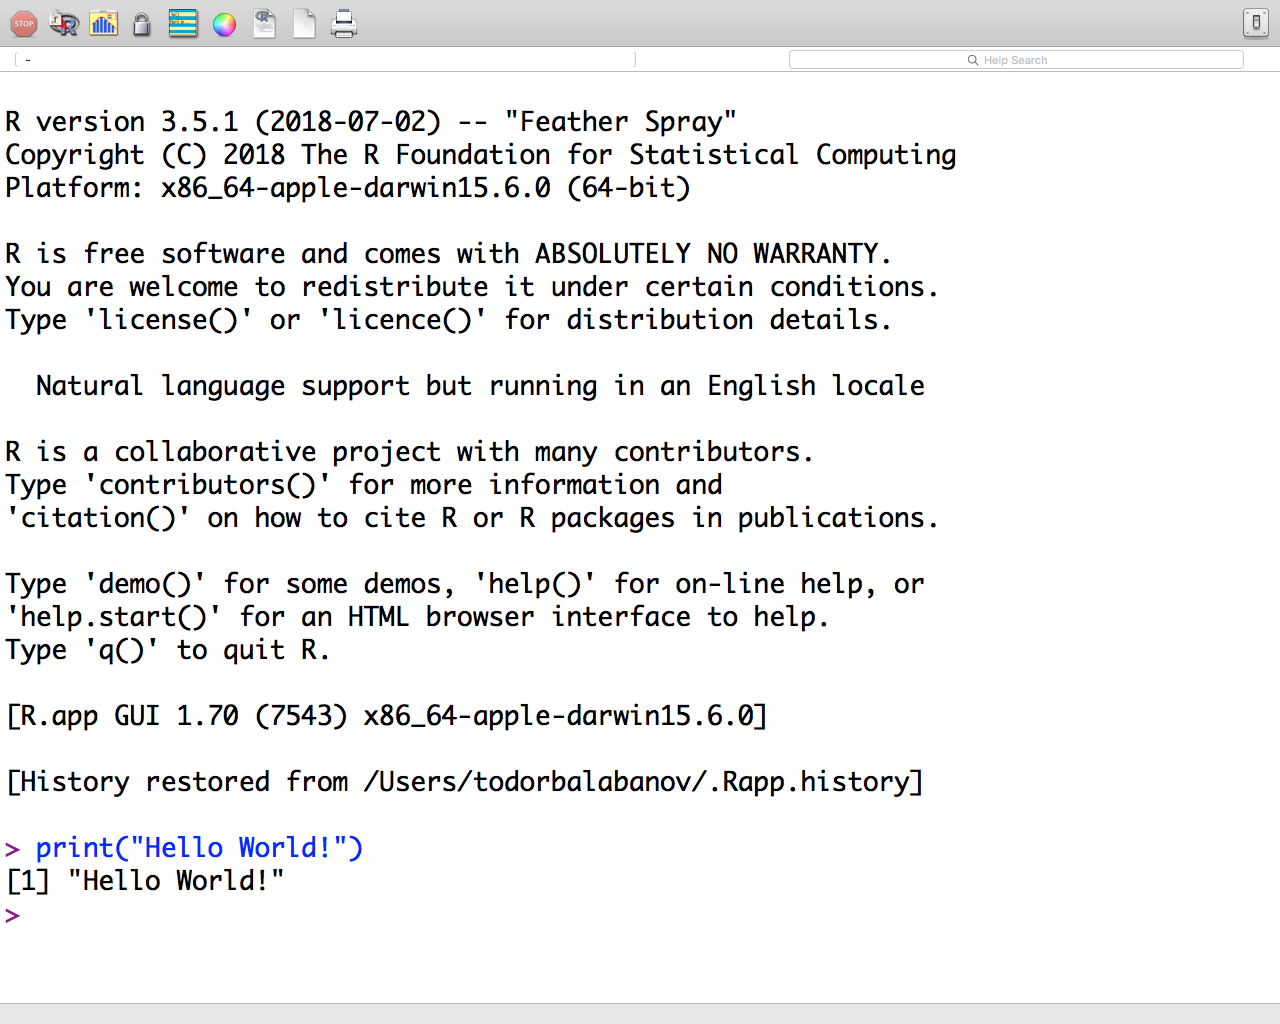
\includegraphics[width=1.0\linewidth]{pic0013}
  \caption{Изпълнение на команда за печат}
\label{figure0013}
\end{figure}
\FloatBarrier

При правилно работеща инсталация изписването на командата за печат би дала резултата показан на Фиг. \ref{figure0013}. Както показва първата примерна команда, има фундаментална разлика в начина, по който работят компилаторите и интерпретаторите. Езици като C/C++ изискват компилация на програмния код до машинни инструкции, които процесорът на компютъра изпълнява. При интерпретативните езици, като PHP, Python, JavaScript и разбира се R, всяка стъпка от програмата се интерпретира в момента на повикването ѝ. По-напредналите потребители на R са добре запознати с начина, по който са изградени библиотеките на езика и знаят добре, че съществува възможност код писан на C/C++ да бъде изпълняван в средата на R. Такава междуезикова връзка най-често се налага при голям обем данни за пресмятане и относително бавни алгоритми, които извършват пресмятането.

\section*{Заключение}

Употребата на всеки програмен продукт преминава през фазите за придобиване на продукта, инсталация и стартиране. Макар и напълно интуитивен, процесът по сваляне, инсталиране и стартиране има своите специфики. 


\newpage
\chapter{Пакетна организация, променливи, основни математически операции в R и типове данни}
\label{chapter02}
\thispagestyle{empty}

Най-голямата сила на продукта R се дължи на хилядите пакети\index{пакети} (софтуерни приставки), създадени от безброй потребители на продукта. Наличните пакети покриват цялата област на статистиката и статистическата обработка на данни. 

Под пакет се разбира софтуерна библиотека от предварително написан програмен код, който има за цел да реши определена задача или група от задачи. Тъй като продуктът R е една отворена система, е важно да се има предвид, че не всички пакети са с еднакво качество. Една част от пакетите са изключително професионално написани, устойчиви са на некоректно използване и имат добра база от поддържащи ги потребители. В същото време друга част от пакетите са създадени с голяма доза добри намерения, но работят бавно, дават дефекти или просто не вършат това, за което са създадени. Голяма част от пакетите са написани от статистици за статистици и това може да доведе до някои странни въпроси при част от потребителите, особено при хора, идващи от индустрията за производство на софтуер.

Настоящото учебно помагало представя само най-основните пакети, достатъчни да бъде изложен материалът свързан с базовите познания по R. Опит да бъдат разгледани всички пакети е непосилен за едно издание, най-вече защото броят и видът на пакетите постоянно се променя.

\section{Инсталиране на пакети}

Съществуват различни начини за инсталиране на пакети в R като най-използваният от тях е чрез команда в конзолата на пакета R.

\begin{figure}[h!]
  \centering
  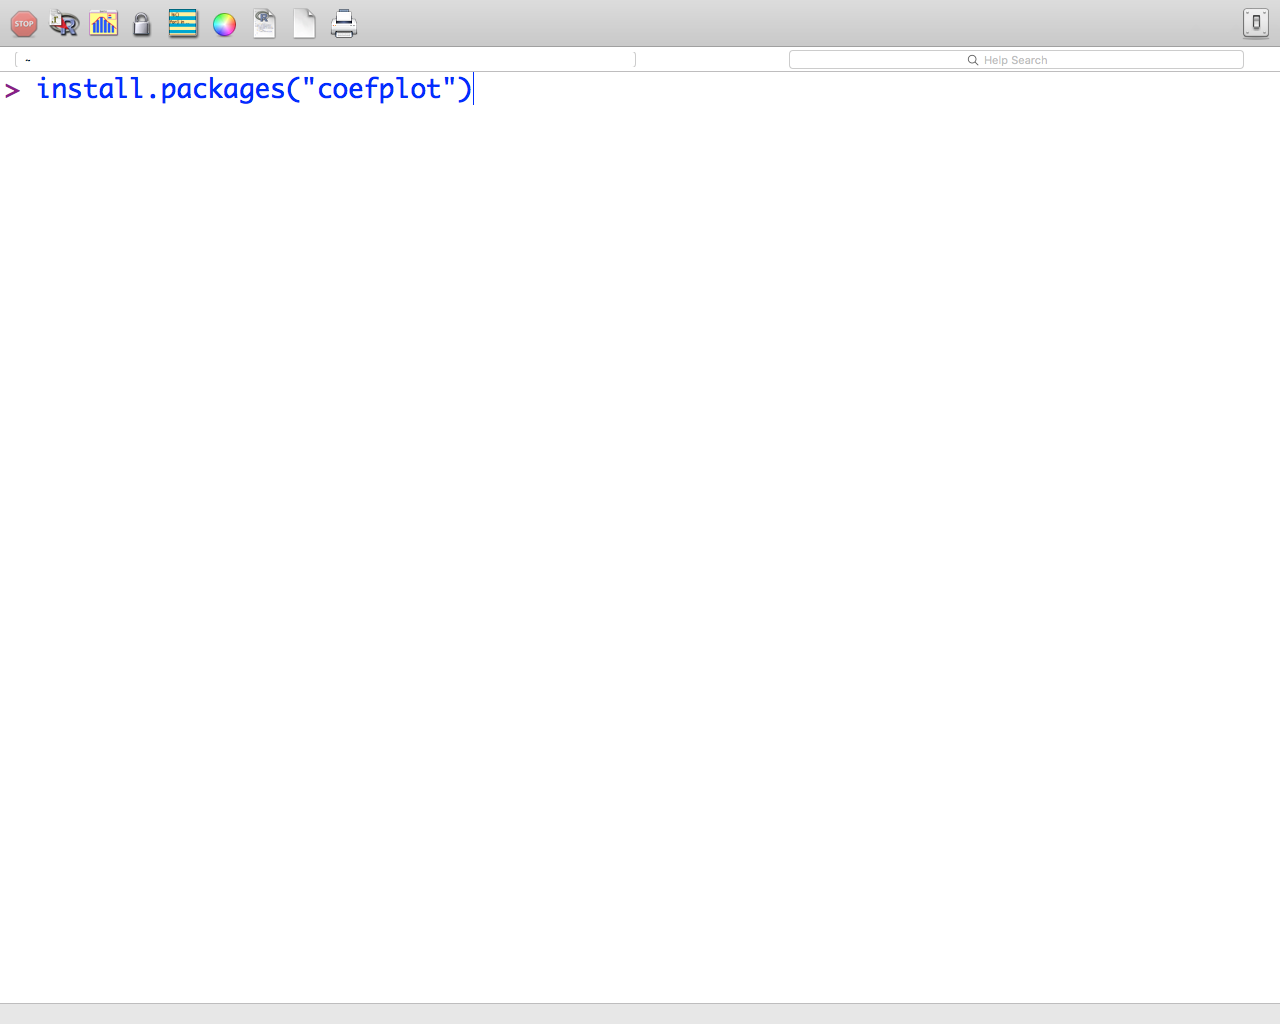
\includegraphics[width=1.0\linewidth]{pic0014}
  \caption{Команда за инсталиране на пакета coefplot}
\label{figure0014}
\end{figure}
\FloatBarrier

За да започне инсталирането на пакет (в случая coefplot) е достатъчно да се изпише командата от Фиг. \ref{figure0014}, със съответното име на пакета като неин параметър.

\begin{figure}[h!]
  \centering
  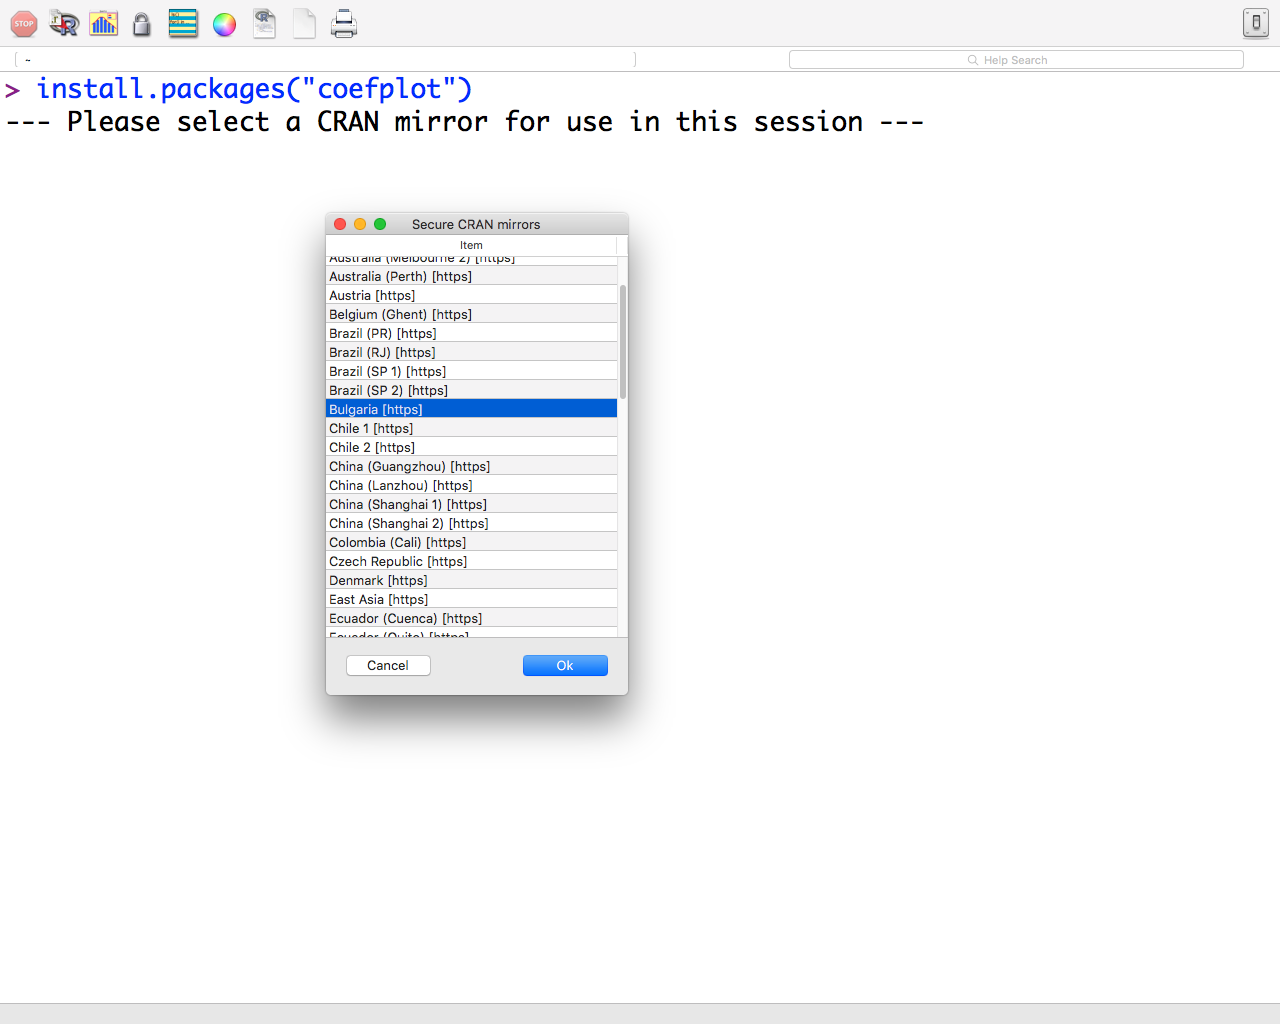
\includegraphics[width=1.0\linewidth]{pic0015}
  \caption{Избор на сървър за изтегляне на пакета}
\label{figure0015}
\end{figure}
\FloatBarrier

Следва избор на сървър за изтегляне на пакета (Фиг. \ref{figure0015}). Разумна стратегия е да се избират сървъри, които териториално се намират в близост до мястото, от което се работи. Това би осигурило малко по-голяма скорост на връзката в Глобалната мрежа.

\begin{figure}[h!]
  \centering
  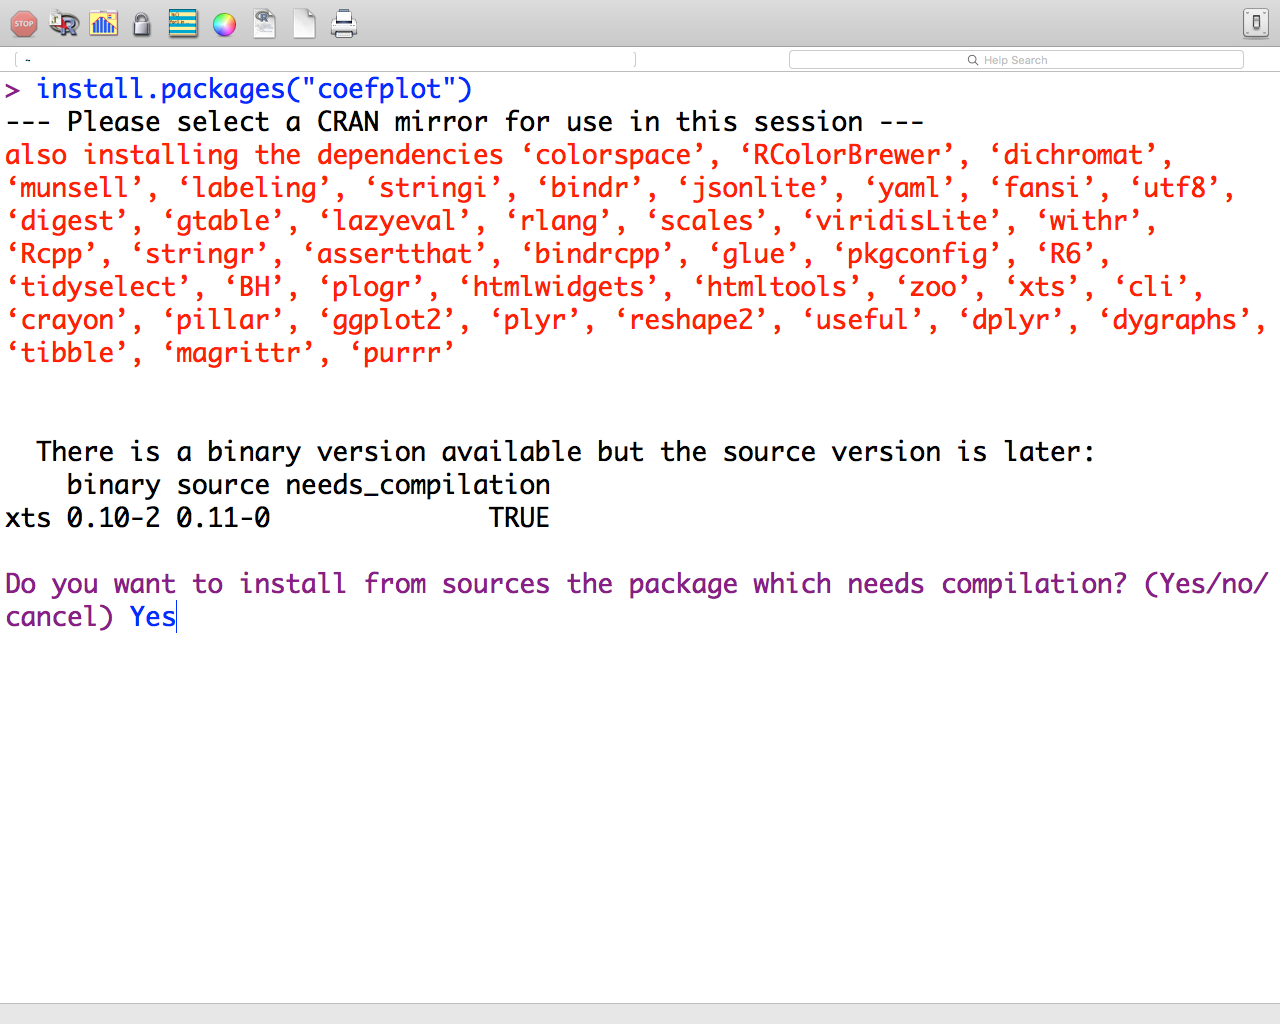
\includegraphics[width=1.0\linewidth]{pic0016}
  \caption{Зависимости между пакетите}
\label{figure0016}
\end{figure}
\FloatBarrier

Често срещан случай е един пакет да има функционална зависимост от други пакети (Фиг. \ref{figure0016}). В такава ситуация е необходимо всички нужни пакети също да бъдат инсталирани. Стратегията при разработка на пакети е те да бъдат предлагани в компилиран (бинарен) вид, но понякога най-новите версии са под формата на програмен код и тогава потребителят има възможност да избере между бинарната версия или версията с програмен код.

\begin{figure}[h!]
  \centering
  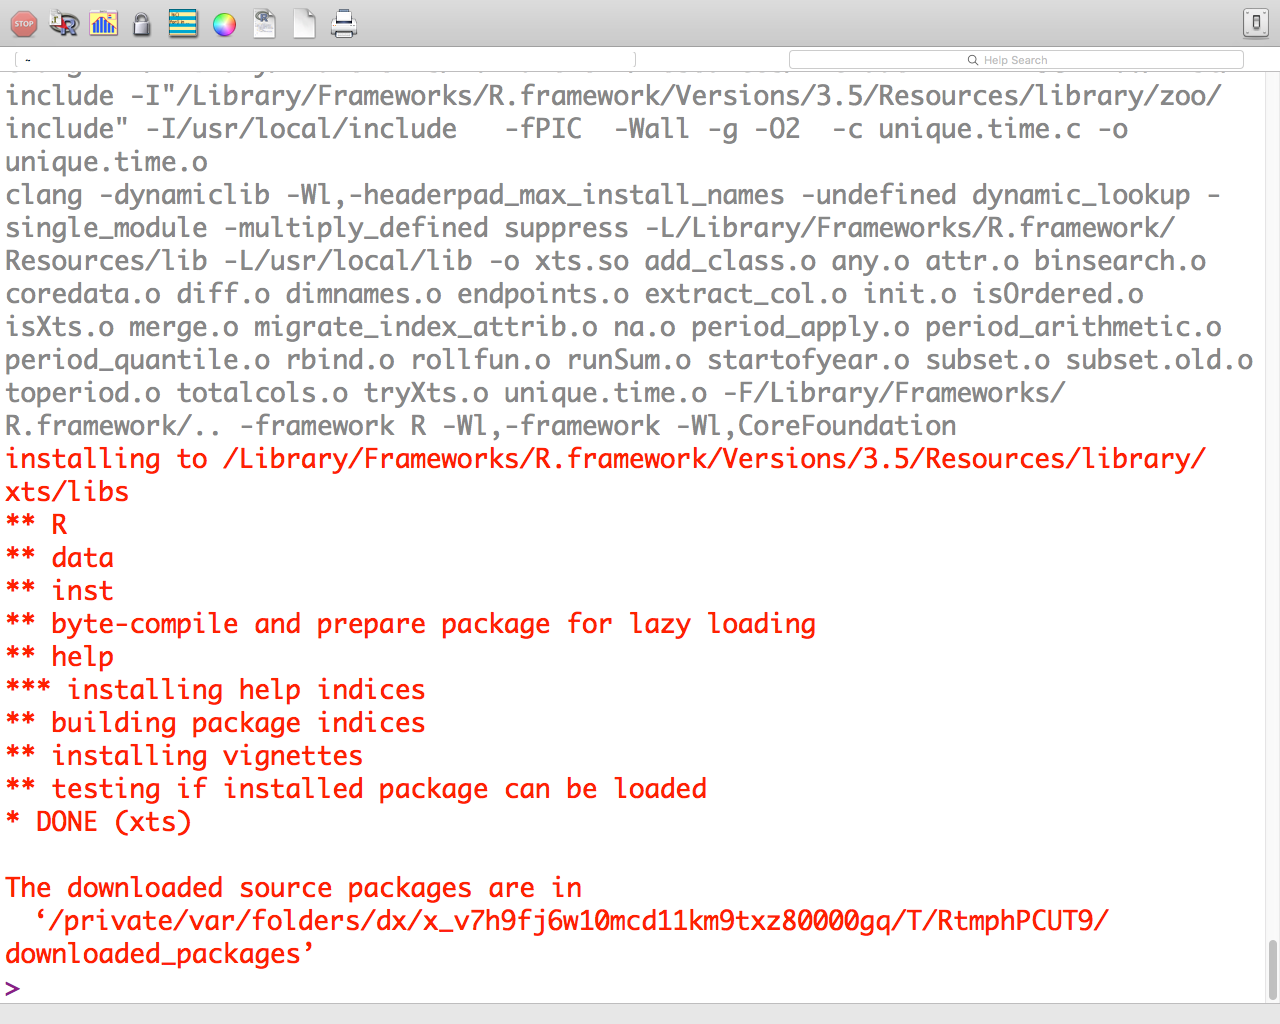
\includegraphics[width=1.0\linewidth]{pic0017}
  \caption{Резултат от инсталацията на пакета}
\label{figure0017}
\end{figure}
\FloatBarrier

Инсталацията на пакета приключва с подробен списък, съдържащ описание на извършените операции (Фиг. \ref{figure0017}).

\begin{figure}[h!]
  \centering
  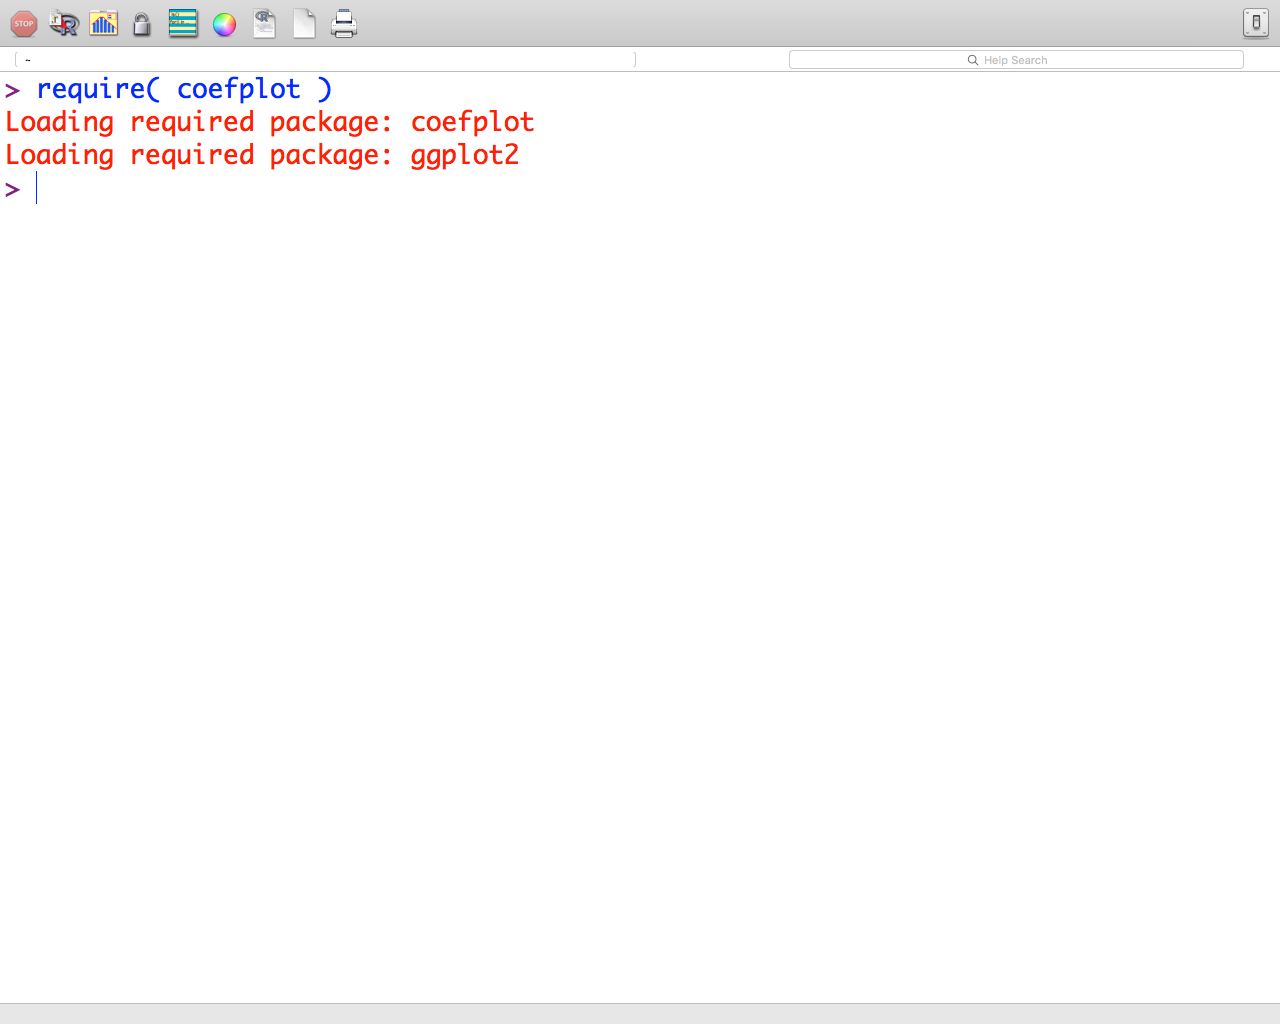
\includegraphics[width=1.0\linewidth]{pic0018}
  \caption{Зареждане на пакета coefplot}
\label{figure0018}
\end{figure}
\FloatBarrier

Дали пакетът е надлежно инсталиран може да се провери с командата require (Фиг. \ref{figure0018}), която зарежда пакета в паметта.

Съществува възможност пакетите да се инсталират под формата на програмен код, директно от хранилищата за програмен код, но за тази цел са нужни подходящите компилатори (най-често C/C++ и Fortran), както и по-задълбочени умения по програмиране. В редки случаи се налага инсталиране на пакета от ZIP файл. При такава ситуация е важно предварително да бъдат инсталирани всички пакети, от които инсталирания пакет зависи.

Премахване на инсталирани пакети става с помощта на командата remove.packages, на която се подава вектор с имената на пакетите, които трябва да бъдат премахнати.

\section{Зареждане на пакети}

За да бъдат използвани пакетите не е достатъчно те да бъдат инсталирани, необходимо е с команда да бъдат включени в текущата сесия от изчисления. R предлага две команди за зареждане на пакети – library и require. И двете изпълняват едно и също нещо – зареждат пакета в общата памет. Разликата е, че require връща TRUE, ако зареждането е било успешно и FALSE при неуспех. Тази възможност е полезна в редките случаи, когато пакетът се зарежда от програмния текст на функция. Подобна практика не е препоръчителна, но R дава такава възможност. И двете функции получават като параметър името на пакета, със или без кавички. Пакетите се зареждат еднократно и остават налични през цялата сесия от изчисления или докато изрично не бъдат премахнати от общата памет.

\begin{figure}[h!]
  \centering
  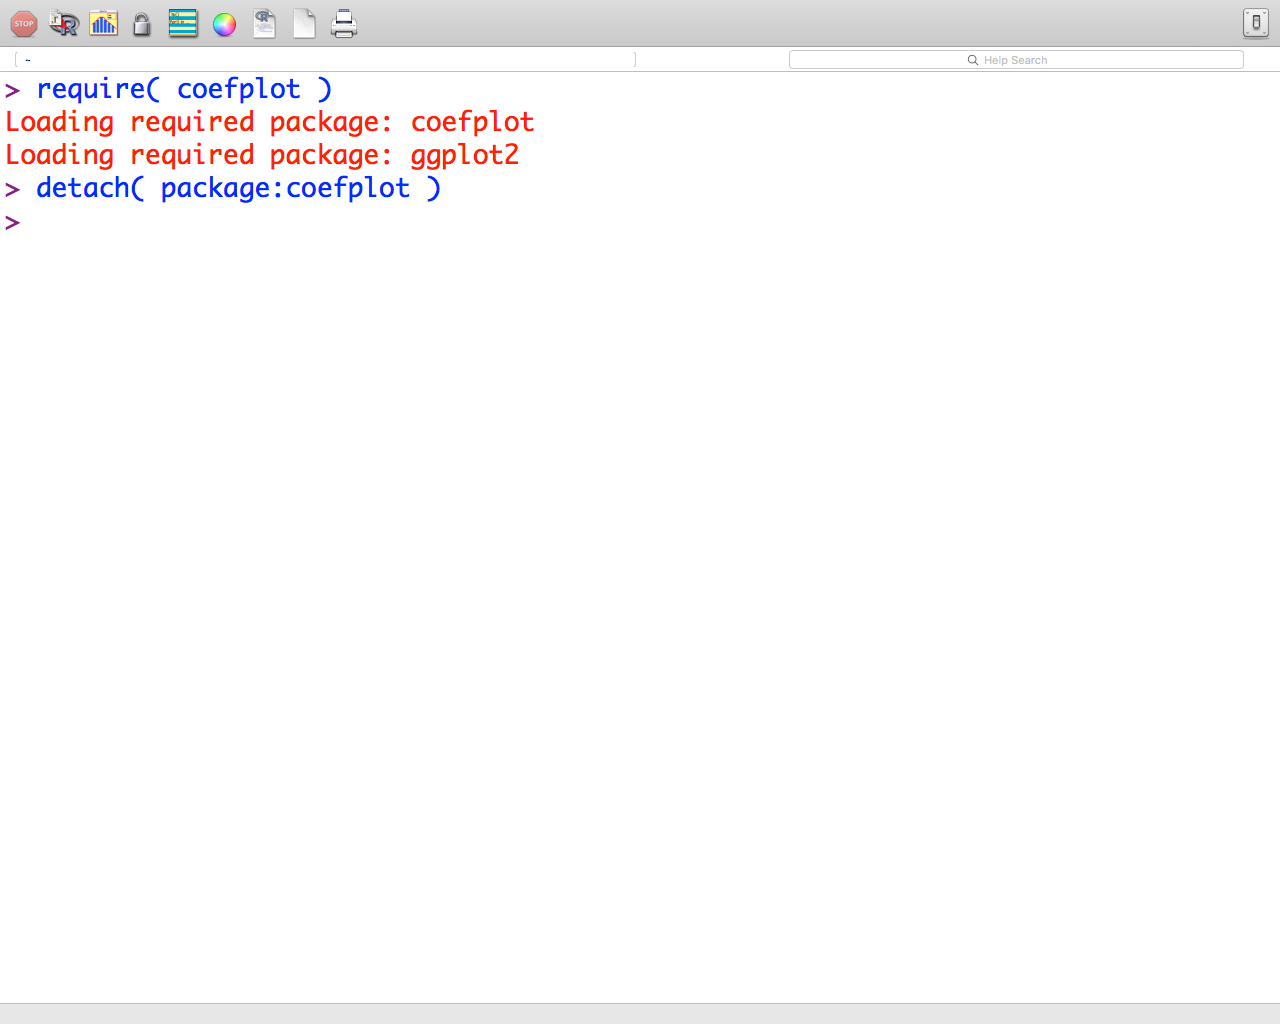
\includegraphics[width=1.0\linewidth]{pic0019}
  \caption{Премахване на пакета coefplot от общата памет}
\label{figure0019}
\end{figure}
\FloatBarrier

Премахването на пакет от общата памет става с командата detach (Фиг. \ref{figure0019}). Същественото при тази команда е, че преди името на пакета се записва думата package.

Тъй като пакетите се разработват основно на доброволни начала, нерядко се случва в различни пакети да има едноименни функции. При подобна колизия на имената решението е да се приложи операцията за принадлежност – двойно двоеточие (::). Когато бъде използвана операцията за принадлежност,  може да не се зарежда пакетът, към който принадлежи функцията.

\section{Основни математически операции}

R позволява да се извършват сложни математически пресмятания\index{математически операции}, но също така може да се използва и за базови математически изчисления. 

\begin{figure}[h!]
  \centering
  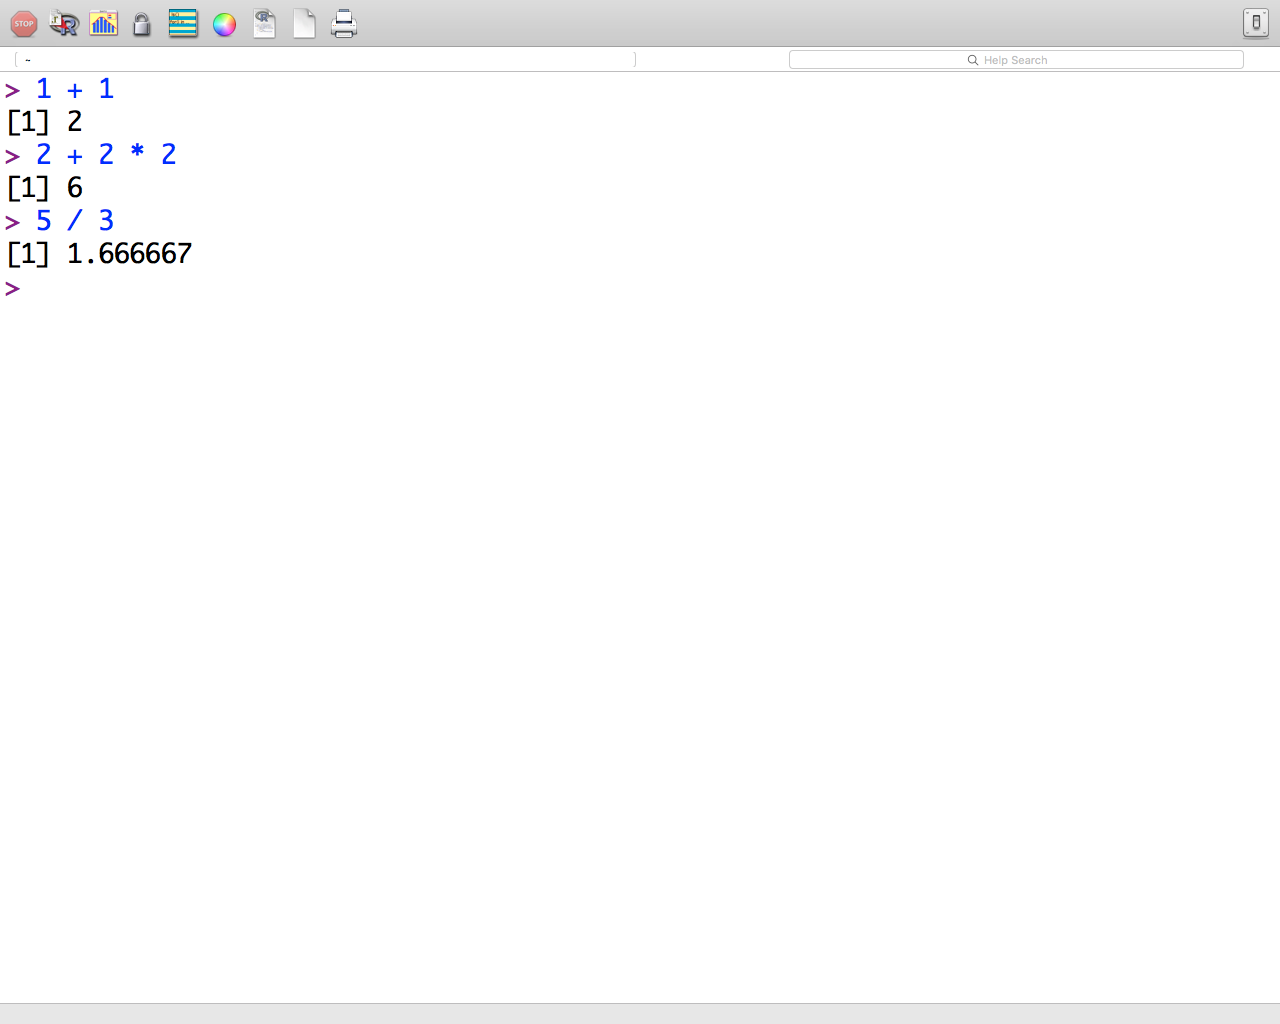
\includegraphics[width=1.0\linewidth]{pic0020}
  \caption{Примерни аритметични операции}
\label{figure0020}
\end{figure}
\FloatBarrier

Най-базовите математически операции са събирането, изваждането, умножението и делението\index{аритметични операции}. Тези операции се изпълняват в R както е показано на Фиг. \ref{figure0020}. Пресмятанията в R се състоят от операции и операнди. Когато няколко операции бъдат обединени, чрез операндите си, се получава математически израз.

\begin{lstlisting}[caption=Събиране, label=listing0001]
1 + 1
\end{lstlisting}

В листинг \ref{listing0001} е демонстрирана операцията за събиране, която има два операнда. Когато става въпрос за математически операции, те имат серия свойства. Като най-съществена характеристика може да се отбележи броят на операндите. Събирането е класически пример за бинарна операция\index{бинарни операции}, тъй като има два операнда (ляв и десен).

\begin{lstlisting}[caption=Унарен минус, label=listing0002]
-5
\end{lstlisting}

В гимназиалния курс по математика не се споменава наличието на унарен плюс, макар и да се учи за унарен минус\index{унарни операции} (Листинг \ref{listing0002}). Унарните плюс и минус променят значението на операнда. В примера от листинг \ref{listing0002}, унарният минус променя значението на числото пет от положително към отрицателно. Тъй като унарният плюс не променя значението на операнда си, масова практика е знакът на унарния плюс да не се записва, това е нещо, което не е възможно с унарния минус. Освен унарни и бинарни операции в някои езици (например C/C++, Java, C\#, PHP и други) съществува една единствена тернарна операция (?:)\index{тернарна операция}, която има смисъла на условния оператор за преход if.

Както бе споменато по-горе, комбинацията от няколко операции и техните операнди водят до съставянето на математически израз\index{математически изрази} (Листинг \ref{listing0003}).

\begin{lstlisting}[caption=Аритметичен израз с две събирания, label=listing0003]
2 + 2 + 2
\end{lstlisting}

Тъй като съвременните изчислителни машини са организирани по такъв начин, че процесорът да извършва само една математическа операция на един такт от пресмятането, става актуален въпросът коя от операциите ще бъде изпълнена първа и коя втора, при положение, че операциите са с еднакъв приоритет. Тъй като в англосаксонската писмена система е прието да се пише и чете от ляво на дясно, то множество математически операции се изпълняват от ляво на дясно. Това се нарича лява асоциативност\index{лява асоциативност} и събирането е точно от тази група операции.

\begin{lstlisting}[caption=Израз за каскадно присвояване, label=listing0004]
a = b = 2
\end{lstlisting}

В гимназиалната математика символът равно се използва за проверка на идентичността между двата операнда, но в компютърните езици символът за равенство има смисъл на операция за присвояване. Това означава, че десният операнд бива присвоен като стойност на левия операнд. При съставянето на математически израз с каскада от присвоявания няма друг вариант, освен първо най-десният операнд да бъде изпълнен и едва накрая най-левият. Това се нарича дясна асоциативност\index{дясна асоциативност} и се използва при значително малък брой от математическите операции.

\begin{lstlisting}[caption=Контекстна зависимост на операциите, label=listing0005]
"abc" + "def"
2 + 2
\end{lstlisting}

Следващата важна характеристика на математическите операции е тяхната контекстна зависимост\index{контекстна зависимост на операциите}. В множество езици събирането на символни низове води до конкатенация (не и в R), докато събирането на числа води до резултат от числено събиране (Листинг \ref{listing0005}).

\begin{lstlisting}[caption=Контекстна зависимост на операцията за делене, label=listing0006]
5 / 3
5.0 / 3.0
\end{lstlisting}

В множество програмни езици (с изключение на R) операцията за деление е контекстно зависима (Листинг \ref{listing0006}). Когато и двата операнда са цели числа, резултатът е целочислено деление, а когато поне един от операндите е дробно число, то резултатът е дробно число.

\begin{lstlisting}[caption=Приоритет на операциите, label=listing0007]
2 + 2 * 2
\end{lstlisting}

Когато в един математически израз участва повече от една операция с еднаква асоциативност, от значение става приоритетът\index{приоритет на операциите} на всяка от тях. Най-често даваният пример е събирането и умножението (Листинг \ref{listing0007}). В случая първо се извършва умножението, тъй като е по-високо приоритетно, а едва след това събирането.

\begin{lstlisting}[caption=Смяна на приоритета, label=listing0008]
(2 + 2) * 2
\end{lstlisting}

В компютърните езици кръглите скоби имат смисъла на операция за промяна на реда, по който ще се извърши пресмятането с цел смяна на приоритета (Листинг \ref{listing0008}).

Последният съществен признак на операциите е в коя група попадат – аритметични, логически, побитови, за сравнение, за присвояване и други.

\section{Типове и променливи}

Повечето съвременни програмни езици организират работата с информация в групи от променливи\index{променливи}. За разлика от строго типизираните езици, в R не се задава тип на променливата\index{типове данни}. Типът на променливата неявно се определя от стойността, която е присвоена към нея. Това позволява да се присвояват дори обекти или функции и означава, че една и съща променлива може да съдържа данни от различни типове в различни моменти от времето.

\subsection{Създаване на променливи}

Променливата се появява в общата памет веднага след първата операция за присвояване, за което съществува цяла група операции за присвояване (Листинг \ref{listing0009}). Променливите в R могат да съдържат в имената си латинските букви и арабските цифри, също символа точка (.) и подчертавка (\_). Имената на променливите не могат да започват с цифра или с подчертавка и са чувствителни към регистъра на буквите (малки/големи)\index{именуване на променливи}.

\begin{lstlisting}[caption=Операции за присвояване, label=listing0009]
a = 1
b <- 2
c = d = 3
e <- f <- 4
assign("g", 5)
a += 6
b -= 7
\end{lstlisting}

Стрелка на ляво (<-) служи за присвояване в R, но в повечето конвенционални програмни езици не присъства\index{операции за присвояване}.

\begin{lstlisting}[caption=Алтернативи за операцията присвояване, label=listing0010]
median(x = 1:10)
median(x <- 1:10)
\end{lstlisting}

Разликата между двете операции си проличава най-ясно при извикването на функции с аргументи (Листинг \ref{listing0010}). В първия случай променливата x не остава в глобалната памет, а изчезва, докато при втория случай променливата x остава в глобалната памет след извикването.

Добра практика е за имена на променливите да се избират съществителни имена, а не еднобуквени имена или съкращения.

\subsection{Премахване на променливи}

\begin{lstlisting}[caption=Премахване на променливи от глобалната памет, label=listing0011]
rm( a )
rm( list=ls() )
\end{lstlisting}

Премахването на променлива от общата памет става с командата rm (Листинг \ref{listing0011}). За да се почисти цялата глобална памет се дава списък с всички променливи, налични в глобалната памет. Въпреки че R извиква Garbage Collector-а, на определени интервали от време с командата gc() може да бъде отправена пряка заявка за освобождаване на ненужно заетата памет.

\subsection{Дискретно представяне на информацията}

Информацията в съвременните изчислителни машини се представя само с две нива 0 (няма сигнал) и 1 (има сигнал)\index{представяне на информацията}. Това е свързано с факта, че съвременните изчислителни машини използват електричество. Наличието само на две различими нива позволява единствено бинарна логика. Една клетка, която може да съдържа 0 или 1 носи един бит информация. Това количество е крайно недостатъчно за изчисленията, които хората имат нужда да правят. За да се разширят възможностите на бинарната логика се използва принципът на супер позицията. Отделните битове се подреждат един до друг и колкото по-вляво е един бит, толкова по-голяма тежест има. В зората на изчислителната техника, макар и да е имало коментари за 4 битови изчислителни машини, такава никога не е създадена за реална употреба. Изборът пада върху 8 битовите машини, които позволяват кодирането на 256 стойности в една машинна дума. Групата от 8 бита, хората наричат байт. Байт е единицата, която масово се използва в ежедневието, също и кратните ѝ форми за MB (мегабайт), GB (гигабайт) или TB (терабайт). Дължината на машинната дума има пряка връзка с размерността на някои от първите типове данни. При 8 битовите машини, в C компилатора, типът int е 8 бита, при 16 битовите е 16 бита, а при 32 битовите е 32 бита. Подредбата на битовете в байтове позволява да се обозначат положителните числа и в езика C това е типът unsigned int. Тъй като в света, който познаваме отрицателни неща няма, то въвеждането на абстракцията за отрицателни числа е нещо неестествено за изчислителните машини и трябва да се избере някаква семантика за различаване на отрицателните от положителните числа. При числата със знак е прието най-старшият разред да бъде използван за знак. По този начин се получава феноменът +0 и -0 нещо, което не се разглежда в гимназиалния курс по математика. Ако най-старшият разряд е високо ниво, а останалите са в ниско се получава отрицателна нула. Ако всички разряди са ниско ниво, то се получава положителна нула. Ограничеността на машинната дума води до серия ограничения при работата с числа. Най-често срещаният проблем е препълването на разрядната решетка. Това е проблем, който и в наши дни се среща в програмния език Java (Листинг \ref{listing0015}).

\begin{lstlisting}[caption=Грешка от препълване при събиране, label=listing0015]
System.out.println( 2 + 2 );
4
System.out.println( 2_000_000_000 + 2_000_000_000 );
-294967296
\end{lstlisting}

Когато се налага да се извършват пресмятания с много големи числа е важно да не се ползват конвенционалните програмни езици, а софтуерни продукти като Matlab, Mathematica или R.

Светът, който познаваме не съдържа концепцията за дробност. Дори елементарните частици са изградени от по-малки елементарни частици. Причината за това е, че живеем в дискретен, а не в непрекъснат свят. Все пак, човекът е въвел концепцията за дробните числа, така че да извършва пресмятания, които да му позволяват по-ясно разбиране на света. Поради чисто физическата си природа разрядната решетка не може да съдържа дробни стойности. Представянето на цели числа е възможно чрез принципа на супер позицията, но той не е приложим при дробните числа. Най-лесният начин да се представи едно дробно число е чрез използването на две цели числа – едно за цялата част и едно за дробната част. Такова представяне е чисто схематично, на практика дробните числа в изчислителните машини се представят по IEEE стандарт. Както може да се препълни цялата част, така може да се препълни и дробната част, което води до проблем познат като underflow. Причината е в това, че компютърът не може да отрази понятието за безкрайност, а между две цели числа (например между 0 и 1) има безкрайно много дробни числа. В изчислителната математика е възприето правилото, че отговорни пресмятания никога не се правят в дробни числа, а се търси вариант за пресмятане с цели числа или чрез пакети за символно пресмятане.

Тъй като в изчислителната техника съществуват само сигнали от ниско и високо ниво, то няма как да бъде кодирана информация за букви или текст. Естественият начин за комуникация между човека и машината са точно текстовете. Поради тази причина в изчислителната техника буквите от естествените езици са номерирани по стандартизирани кодови таблици. Две от най-популярните кодови таблици са ASCII и UTF-8. ASCII стандартът е силно ограничен и не позволява кодирането на повечето естествени езици, поради тази причина е създаден стандартът UTF-8 (един от най-разпространените в наше време), който позволява достатъчно икономично да бъдат представени символите от азбуките на познатите естествени езици.

\subsection{Числени стойности}

Условно R спада към групата на безтиповите езици, но всяка променлива вътрешно съхранява информация, която определя типа на данните. Възможни са различни типове данни, но най-използваните са numeric, character (включително символни низове), Date/POSIXct (астрономическо време) и logical (TRUE/FALSE).

\begin{lstlisting}[caption=Проверка за типа на променливата, label=listing0012]
a = 5
class( a )
[1] "numeric"
\end{lstlisting}

С помощта на функцията class (Листинг \ref{listing0012}) може да се провери типът на променливата. Тъй като R основно се използва за изчисления, то най-употребяваният тип данни са числовите данни\index{числени типове}. В този аспект numeric съответства на типовете float и double в другите конвенционални езици за програмиране. Този тип данни се използва за цели и дробни числа, както и за нулата. Това е типът по подразбиране, който се задава на променливата при числено присвояване.

\begin{lstlisting}[caption=Проверка за типа numeric, label=listing0013]
is.numeric( a )
[1] TRUE
\end{lstlisting}

Проверката за numeric типа се извършва както е показано в листинг \ref{listing0013}.

\begin{lstlisting}[caption=Използване на целочислен тип, label=listing0014]
b <- 6L

class( b )
[1] "integer"

is.numeric( b )
[1] TRUE

is.integer( b )
[1] TRUE

is.integer( a )
[1] FALSE
\end{lstlisting}

R допуска използването само на цели числа, чрез типа integer. За да бъде указан типът integer към числото се добавя буквата L (Листинг \ref{listing0014}).

\subsection{Символни низове}

\begin{lstlisting}[caption=Символни низове в R, label=listing0016]
s1 <- "Simple text."
s1
[1] "Simple text."

class( s1 )
[1] "character"

s2 <- factor( "Another simple text." )
s2
[1] Another simple text.
Levels: Another simple text.

class( s2 )
[1] "factor"
\end{lstlisting}

За символни низове\index{символни низове} има два възможни варианта, които са показани на листинг \ref{listing0016}. Символните низове в R са чувствителни към малки и големи букви. Фактор е специален символен низ, който намира приложение при векторите.

\begin{lstlisting}[caption=Дължина на символен низ или числена стойност, label=listing0017]
nchar( s1 )
[1] 12

nchar( s2 )
Error in nchar(s2) : 'nchar()' requires a character vector

nchar( a )
[1] 1
\end{lstlisting}

Дължината на символен низ или числена стойност може да се определи с функцията nchar, която обаче не е приложима за променливите от тип фактор (Листинг \ref{listing0017}).

\subsection{Астрономическо време}

При статистическата обработка на данни много често измерванията се извършват в точно определен момент от времето. Това налага наличието на възможности за обработка на астрономическо време\index{типове за астрономическо време}. Работата с астрономическо време носи своите трудности поради множество фактори. От една страна има множество часови зони. Също така различните месеци в годината имат различен брой дни. Някои години се различават по брой дни. В една част от държавите се минава към лятно часово време и зимно часово врем, докато в другите това не се прави.

\begin{lstlisting}[caption=Типове данни за време, label=listing0018]
d1 <- as.Date("1979-04-21")
d1
[1] "1979-04-21"

class( d1 )
[1] "Date"

as.numeric( d1 )
[1] 3397

d2 <- as.POSIXct("1980-02-12 05:25")
d2
[1] "1980-02-12 05:25:00 EET"

class( d2 )
[1] "POSIXct" "POSIXt" 

as.numeric( d2 )
[1] 319173900
\end{lstlisting}

В R най-често използваните типове за астрономическо врем са Date и POSIXct (Листинг \ref{listing0018}). Типът Date съхранява само информацията за дата, докато типът POSIXct съхранява информация за датата и за часа. Вътрешното представяне на Date е брой дни от 1 януари 1970 година, а вътрешното представяне на POSIXct е брой секунди от 00:00:00 на 1 януари 1970 година. Тъй като боравенето с информация за астрономическо време може да бъде относително сложно, то за тази цел са налични два помощни пакета - lubridate и chron.

\subsection{Логически стойности}

Логическият тип данни\index{логически тип данни} е също често използван и е в групата на простите типове данни. Променливите съдържат стойности FALSE или TRUE. На предефинираните константи са присвоени числени стойности 0 за FALSE и 1 за TRUE.

\begin{lstlisting}[caption=Логически тип данни, label=listing0019]
x1 <- TRUE
x1
[1] TRUE

class( x1 )
[1] "logical"

is.logical( x1 )
[1] TRUE

as.numeric( x1 )
[1] 1

x2 <- F
x2
[1] FALSE

class( x2 )
[1] "logical"

is.logical( x2 )
[1] TRUE

as.numeric( x2 )
[1] 0
\end{lstlisting}

Освен пълното изписване на булевите стойности, може да се използват променливите T и F, но те не са препоръчителни, тъй като могат да бъдат предефинирани и това да доведе до сериозни логически грешки (Листинг \ref{listing0019}).

\begin{lstlisting}[caption=Операции за сравнение, label=listing0020]
2 == 3
[1] FALSE

5 != 6
[1] TRUE

"Peter" == "Ivan"
[1] FALSE
\end{lstlisting}

Логическият тип данни най-често се получава в следствие на операциите за сравнение (Листинг \ref{listing0020}).

\section*{Заключение}

В тази глава са разгледани основните принципи за работа с пакети, работата с променливи, най-съществените операции с данни и някои от базовите типове данни.

\newpage
\chapter{Сложни структури от данни и викане на функции}
\label{chapter03}
\thispagestyle{empty}

\section{Извикване на функции}

Функциите са последователност от инструкции, обособени като едно цяло, така че да са подходящи за многократно извикване. Функциите приемат входящи параметри, могат да имат върната стойност, а символът диез (\#) се използва в началото на ред за коментар. Организацията на програмния текст във функции позволява лесна четимост и по-лесно откриване на програмни дефекти (бъгове). По своята същност командите в конзолата на R са функции, които потребителят извиква. Поради този факт е важно да се знаят възможностите за работа с функции\index{извикване на функции}. За разлика от масово наложените езици за обектно-ориентирано програмиране, в R функциите са по-съществени от обектите.

\begin{lstlisting}[caption=Извикване на функции, label=listing0029]
x <- c(1, 2, 3, 5, 6, 7, 8, 9)
x
[1] 1 2 3 5 6 7 8 9

mean( x )
[1] 5.125

median( x )
[1] 5.5

sd( x )
[1] 2.900123
\end{lstlisting}

Листинг \ref{listing0029} демонстрира извикването на три функции, които получават като единствен аргумент вектор от числени стойности. По-сложните функции може да имат повече аргументи\index{аргументи на функции} и те да се подават по различен начин.

Всяка функция, която е достъпна в R, има съпровождаща документация\index{документация на функции}, но качеството на тази документация може да варира според уменията на автора ѝ. Най-бързият начин за достъп до информацията е чрез поставяне на въпросителен (?) пред името на функцията (Листинг \ref{listing0030}).

\begin{lstlisting}[caption=Документация за функциите, label=listing0030]
? mean
?? mean
? median
?? median
? sd
?? sd
\end{lstlisting}

Един въпросителен отваря информацията в локален прозорец, а два въпросителни отварят уеб страницата, съдържаща документацията на функцията.

\begin{lstlisting}[caption=Документация за операции, label=listing0031]
? `+`
? `-`
? `*`
? `/`
\end{lstlisting}

За голяма част от операциите също може да се получи информация по сходен начин (Листинг \ref{listing0031}), но операцията\index{документация на операции} трябва да бъде оградена със символа апостроф (\`).

\begin{lstlisting}[caption=Частично търсене, label=listing0032]
apropos( "med" )
[1] "elNamed"        "elNamed<-"      "median"         "median.default"
[5] "medpolish"      "runmed"
\end{lstlisting}

Често потребителите имат идея каква функция търсят, но не се досещат за точното изписване на името ѝ. В такива ситуации е полезна възможността за частично търсене\index{частично търсене}, която предоставя функцията apropos (Листинг \ref{listing0032}).

\section{Вектори}

Векторът\index{вектори} е колекция от елементи, които са от един и същи тип (Листинг \ref{listing0021}). 

\begin{lstlisting}[caption=Вектор от числа и вектор от символни низове, label=listing0021]
v1 <- c(1, 3, 2, 1, 5)
v2 <- c("Peter", "Ivan", "Geroge")
\end{lstlisting}

Векторите в R имат значителна роля за езика, тъй като R е векторизиран език, което го прави различен от конвенционалните програмни езици, като C/C++, C\# или Java. Това означава, че всяка математическа операция се изпълнява върху целия вектор и не е нужно да се обикалят отделните елементи един по един (Листинг \ref{listing0022}). За разлика от математическата концепция, в R векторите не се делят на вектор-стълб или вектор-ред. При нужда от вектор-ред или вектор-стълб може да се използват матрици с единична стойност на един от размерите.

\begin{lstlisting}[caption=Базови операции над вектори, label=listing0022]
x <- c(1, 2, 3, 4, 5, 6, 7, 8, 9, 10)
x
[1]  1  2  3  4  5  6  7  8  9 10

x * 5
[1]  5 10 15 20 25 30 35 40 45 50

x + 3
[1]  4  5  6  7  8  9 10 11 12 13

x - 4
[1] -3 -2 -1  0  1  2  3  4  5  6

x / 5
[1] 0.2 0.4 0.6 0.8 1.0 1.2 1.4 1.6 1.8 2.0

x ^ 3
[1]    1    8   27   64  125  216  343  512  729 1000

sqrt( x )
[1] 1.000000 1.414214 1.732051 2.000000 2.236068 2.449490 2.645751 2.828427
[9] 3.000000 3.162278
\end{lstlisting}

Основният начин за създаване на вектор е чрез функцията c, като названието ѝ идва от combine (комбиниране на елементи), но също е възможно да се използва и алтернативен запис (Листинг \ref{listing0023}).

\begin{lstlisting}[caption=Алтернативен синтаксис за създаване на вектори, label=listing0023]
1:10
[1] 1 2 3 4 5 6 7 8 9 10

10:1
[1] 10 9 8 7 6 5 4 3 2 1

-2:3
[1] -2 -1 0 1 2 3

5:-7
[1] 5 4 3 2 1 0 -1 -2 -3 -4 -5 -6 -7
\end{lstlisting}

Когато двата операнда на операцията са вектори\index{операции с вектори} с еднакви дължини, то операцията се прилага на всичките елементи по двойки (Листинг \ref{listing0024}).

\begin{lstlisting}[caption=Операции между вектори с еднаква дължина, label=listing0024]
x <- 1:10
y <- -10:-1

nchar( x )
[1] 1 1 1 1 1 1 1 1 1 2

nchar( y )
[1] 3 2 2 2 2 2 2 2 2 2

x + y
[1] -9 -7 -5 -3 -1  1  3  5  7  9

x - y
[1] 11 11 11 11 11 11 11 11 11 11

x * y
[1] -10 -18 -24 -28 -30 -30 -28 -24 -18 -10

x / y
[1]  -0.1000000  -0.2222222  -0.3750000  -0.5714286  -0.8333333  -1.2000000
[7]  -1.7500000  -2.6666667  -4.5000000 -10.0000000

x ^ y
[1] 1.000000e+00 1.953125e-03 1.524158e-04 6.103516e-05 6.400000e-05
[6] 1.286008e-04 4.164931e-04 1.953125e-03 1.234568e-02 1.000000e-01

x > y
[1] TRUE TRUE TRUE TRUE TRUE TRUE TRUE TRUE TRUE TRUE
\end{lstlisting}

Когато векторите са с различна дължина, по-късият вектор се превърта и се започва от началото му. Функцията nchar показва колко символа са необходими за изписването на всеки от елементите.

\begin{lstlisting}[caption=Проверка дали някоя или всички стойности от вектора отговарят на определено условие, label=listing0025]
any(x+y < 0)
[1] TRUE

all(x+y < 0)
[1] FALSE
\end{lstlisting}

При група от проверки може да се установи дали всички елементи на вектора изпълняват определено условие или поне някои елементи го изпълняват (Листинг \ref{listing0025}).

\begin{lstlisting}[caption=Достъп до отделни елементи във вектор, label=listing0026]
x[ 1 ]
[1] 1

x[ 2:3 ]
[1] 2 3

x[ c(2,5,7) ]
[1] 2 5 7
\end{lstlisting}

Достъп до отделни елементи във вектор може да се осъществи по индекс или множество от индекси (Листинг \ref{listing0026}).

\begin{lstlisting}[caption=Имена на елементите във вектора, label=listing0027]
z <- c(One=1, Two=2, Three=3)
z
  One   Two Three 
    1     2     3 

names( z )
[1] "One"   "Two"   "Three"
\end{lstlisting}

R позволява на елементите във вектора да се поставят имена (Листинг \ref{listing0027}).

\begin{lstlisting}[caption=Трансформация на вектор във фактор, label=listing0028]
e <- c("High School", "College", "Masters", "Doctorate")
e

[1] "High School" "College"     "Masters"     "Doctorate"  
f1 <- as.factor( e )
f1
[1] High School College     Masters     Doctorate  
Levels: College Doctorate High School Masters

as.numeric( f1 )
[1] 3 1 4 2

f2 <- factor(c("High School", "College", "Masters", "Doctorate"), 
		 levels=c("High School", "College", "Masters", "Doctorate"),
		 ordered=TRUE)
f2
[1] High School College     Masters     Doctorate  
Levels: High School < College < Masters < Doctorate

as.numeric( f2 )
[1] 1 2 3 4
\end{lstlisting}

Вектор може да бъде трансформиран във фактор\index{фактори} с помощта на функции за трансформация (Листинг \ref{listing0028}). Факторът е тип данни, при който всяка стойност се среща само по един път. Някои множества са неподредени (както е f1) и при тях няма значение редът на елементите, докато при подредените множества (както е f2) редът на елементите има значение . Функцията factor позволява изрично да се зададе какъв е редът на елементите. Факторът е значително по-икономичен на памет от вектора, тъй като се запазват единствено числените стойности на отделните елементи, но пък използването му може да доведе до трудни за откриване логически грешки.

\begin{lstlisting}[caption=Вектори с латинските букви, label=listing0051]
letters
 [1] "a" "b" "c" "d" "e" "f" "g" "h" "i" "j" "k" "l" "m" "n" "o" "p" "q" "r"
[19] "s" "t" "u" "v" "w" "x" "y" "z"

LETTERS
 [1] "A" "B" "C" "D" "E" "F" "G" "H" "I" "J" "K" "L" "M" "N" "O" "P" "Q" "R"
[19] "S" "T" "U" "V" "W" "X" "Y" "Z"
\end{lstlisting}

В R има два специално предефинирани вектора, които съдържат буквите от латинската азбука (Листинг \ref{listing0051}).

\section{Липсващи стойности}

Липсващи стойности\index{липсващи стойности} в данните е ежедневен проблем за хората обработващи статистическа информация. Причините за липсващите данни могат да произлизат от различни обстоятелства, например пропуснато измерване или дефектирал датчик. R дава две възможности за обозначаване на липсващи стойности в данните (NA и NULL). Макар да имат сходно значение, тези две стойности водят до различни резултати при различните пресмятания.

Когато има липсващи стойности в данните съществуват множество начини този факт да бъде отразен. В някои комплекти данни се записва недопустима числена стойност или се използва някаква символна комбинация. В езика R е възприето липсващите стойности да се обозначават с NA (Листинг \ref{listing0033}).

\begin{lstlisting}[caption=Липсващи стойности, label=listing0033]
x <- c(1, NA, 3, NA, 5)
x
[1]  1 NA  3 NA  5

is.na( x )
[1] FALSE  TRUE FALSE  TRUE FALSE

mean( x )
[1] NA

median( x )
[1] NA

sd( x )
[1] NA
\end{lstlisting}

Значението на NULL е липса, а не изпусната стойност, поради тази причина векторът се редуцира с толкова елементи, колкото NULL стойности има в него (Листинг \ref{listing0034}).

\begin{lstlisting}[caption=Липсващи стойности, label=listing0034]
y <- c(1, NULL, 3, NULL, 5)
y
[1] 1 3 5

is.na( y )
[1] FALSE FALSE FALSE

mean( y )
[1] 3

median( y )
[1] 3

sd( y )
[1] 2

is.null( y )
[1] FALSE
\end{lstlisting}

Тъй като на практика векторът се редуцира с броя на NULL стойностите си, то функцията is.null не е векторизирана, а се отнася за целия обект.

\section{Рамкирани данни}

Рамкираните данни\index{рамкирани данни} (data.frame) са една от най-полезните структури от данни в езика R. Най-интуитивната аналогия за рамкирани данни е един лист (data sheet) в Microsft Excel, състоящ се от колони и редове. В термините на статистиката, всяка колона е наблюдавана променлива, а всеки ред е едно конкретно наблюдение (измерване). В термините на R, всяка колона е вектор, а дължината на всичките вектори е една и съща. По този начин всяка колона може да съдържа различни типове данни. Също така, в рамките на една колона всички елементи са от един и същи тип.

Съществуват множество начини да се създадат рамкирани данни, но най-лесният е с функцията data.frame.

\begin{lstlisting}[caption=Създаване на рамкирани данни, label=listing0035]
x <- sample(1:5)
x
[1] 4 1 3 2 5

y <- sample(-2:2)
y
[1]  0 -2  1 -1  2

q <- c("Football", "Basketball", "Volleyball", "Handball", "Rugby")
q
[1] "Football"   "Basketball" "Volleyball" "Handball"   "Rugby"

df1 <- data.frame(x, y, q)
df1
  x  y          q
1 4  0   Football
2 1 -2 Basketball
3 3  1 Volleyball
4 2 -1   Handball
5 5  2      Rugby
\end{lstlisting}

Листинг \ref{listing0035} демонстрира създаването на рамкирани данни от два вектора с числа (sample служи за разбъркване на стойностите по случаен начин) и един вектор със символни низове. Така получената структура е с размери 5x3 и се състои от три вектора. Имената на колоните се вземат служебно, но е възможно те да бъдат определени при създаването на самата структура (Листинг \ref{listing0036}).

\begin{lstlisting}[caption=Създаване на рамкирани данни с имена на колоните, label=listing0036]
df2 <- data.frame(First=x, Second=y, Sport=q)
rownames( df2 ) <- c("One", "Two", "Three", "Four", "Five")
df2
      First Second      Sport
One       4      0   Football
Two       1     -2 Basketball
Three     3      1 Volleyball
Four      2     -1   Handball
Five      5      2      Rugby
\end{lstlisting}

Рамкираните данни имат множество атрибути, като най-съществените са броя редове и броя колони (Листинг \ref{listing0037}). Атрибутите имат съществено значение при прилагането на различните алгоритми за статистически анализ.

\begin{lstlisting}[caption=Атрибути на рамкираните данни, label=listing0037]
nrow( df1 )
[1] 5

ncol( df1 )
[1] 3

dim( df1 )
[1] 5 3

names( df2 )
[1] "First"  "Second" "Sport"

rownames( df2 )
[1] "One"   "Two"   "Three" "Four"  "Five" 

head(df1, n=3)
  x  y          q
1 4  0   Football
2 1 -2 Basketball
3 3  1 Volleyball

tail(df1, n=3)
  x  y          q
3 3  1 Volleyball
4 2 -1   Handball
5 5  2      Rugby

class( df1 )
[1] "data.frame"
\end{lstlisting}

Също така, може да се проверят имената на колоните и имената на редовете, с функцията head за първите няколко реда, а с функцията tail за последните няколко реда.

\begin{lstlisting}[caption=Фактори в рамковите данни, label=listing0038]
df2[1, 2]
[1] 0

df2[3, 2:3]
      Second      Sport
Three      1 Volleyball

df2$Sport
[1] Football   Basketball Volleyball Handball   Rugby     
Levels: Basketball Football Handball Rugby Volleyball

class( df2$Sport )
[1] "factor"

df2$Sport[1:2]
[1] Football   Basketball
Levels: Basketball Football Handball Rugby Volleyball

df2[3, ]
      First Second      Sport
Three     3      1 Volleyball

df2[, c("First", "Sport")]
      First      Sport
One       4   Football
Two       1 Basketball
Three     3 Volleyball
Four      2   Handball
Five      5      Rugby
\end{lstlisting}

Рамкираните данни позволяват достъп до елементите като индекси\index{достъп по индекс} на двумерен масив или директно с адресиране на конкретна колона (Листинг \ref{listing0038}). Достъпът до цял ред става без указване на колона. За достъп до колоните по име се съставя вектор с имената на колоните.

\begin{lstlisting}[caption=Вътрешно представяне на факторите, label=listing0039]
f1 <- factor( c("Sofia", "Plovdiv", "Varna", "Burgas", "Ruse") )
f1
[1] Sofia   Plovdiv Varna   Burgas  Ruse   
Levels: Burgas Plovdiv Ruse Sofia Varna

model.matrix(~f1 - 1)
  f1Burgas f1Plovdiv f1Ruse f1Sofia f1Varna
1        0         0      0       1       0
2        0         1      0       0       0
3        0         0      0       0       1
4        1         0      0       0       0
5        0         0      1       0       0
attr(,"assign")
[1] 1 1 1 1 1
attr(,"contrasts")
attr(,"contrasts")$f1
[1] "contr.treatment"
\end{lstlisting}

Факторите са малко по-различни от векторите, за да се проследи вътрешното им представяне в рамкираните данни може да се приложи функцията model.matrix (Листинг \ref{listing0039}).

\section{Списъци}

В някои ситуации е нужно да се ползва контейнер, който да съдържа обекти от различни типове. В R това се постига със списъчните структури. Този тип структури могат да съдържат голям брой и различни по тип елементи. Списъците се създават с функцията list (Листинг \ref{listing0040}).

\begin{lstlisting}[caption=Създаване на списък, label=listing0040]
l1 <- list(1, 2, 3, 4, 5)
l1
[[1]]
[1] 1

[[2]]
[1] 2

[[3]]
[1] 3

[[4]]
[1] 4

[[5]]
[1] 5
\end{lstlisting}

Всеки елемент в списъка е самостоятелен (Листинг \ref{listing0040}), но е възможно да има и списък с единствен елемент, който е вектор (Листинг \ref{listing0041}).

\begin{lstlisting}[caption=Вектор в списък, label=listing0041]
l2 <- list( c(1, 2, 3, 4, 5) )
l2
[[1]]
[1] 1 2 3 4 5
\end{lstlisting}

Разнородни елементи на списък са показани в Листинг \ref{listing0042}.

\begin{lstlisting}[caption=Списък с разнородни данни, label=listing0042]
l3 <- list( df2, 1:5, l1 )
l3
[[1]]
      First Second      Sport
One       4      0   Football
Two       1     -2 Basketball
Three     3      1 Volleyball
Four      2     -1   Handball
Five      5      2      Rugby

[[2]]
[1] 1 2 3 4 5

[[3]]
[[3]][[1]]
[1] 1

[[3]][[2]]
[1] 2

[[3]][[3]]
[1] 3

[[3]][[4]]
[1] 4

[[3]][[5]]
[1] 5
\end{lstlisting}

По подобие на рамкираните данни, списъците също могат да съдържат наименования на елементите си (Листинг \ref{listing0043}).

\begin{lstlisting}[caption=Названия на елементите в списъка, label=listing0043]
names( l3 ) <- c("Frame", "Vector", "Element")
l3
$Frame
      First Second      Sport
One       4      0   Football
Two       1     -2 Basketball
Three     3      1 Volleyball
Four      2     -1   Handball
Five      5      2      Rugby

$Vector
[1] 1 2 3 4 5

$Element
$Element[[1]]
[1] 1

$Element[[2]]
[1] 2

$Element[[3]]
[1] 3

$Element[[4]]
[1] 4

$Element[[5]]
[1] 5
\end{lstlisting}

Достъпът до елементите на списъка може да стане по индекс\index{достъп по индекс} или по название на елемента (Листинг \ref{listing0044}).

\begin{lstlisting}[caption=Достъп до елементите на списъка, label=listing0044]
l3[ 1 ]
$Frame
      First Second      Sport
One       4      0   Football
Two       1     -2 Basketball
Three     3      1 Volleyball
Four      2     -1   Handball
Five      5      2      Rugby

l3[ "Frame" ]
$Frame
      First Second      Sport
One       4      0   Football
Two       1     -2 Basketball
Three     3      1 Volleyball
Four      2     -1   Handball
Five      5      2      Rugby
\end{lstlisting}

Чрез вложено позоваване може да се достъпи конкретен елемент (Листинг \ref{listing0045}). Тъй като сложните структури от данни могат да съдържат на свой ред сложни структури от данни, вложеното позоваване може да добие твърде неприветлив вид.

\begin{lstlisting}[caption=Вложено позоваване, label=listing0045]
l3[[1]]
      First Second      Sport
One       4      0   Football
Two       1     -2 Basketball
Three     3      1 Volleyball
Four      2     -1   Handball
Five      5      2      Rugby

l3[["Frame"]]$Sport
[1] Football   Basketball Volleyball Handball   Rugby     
Levels: Basketball Football Handball Rugby Volleyball
\end{lstlisting}

Добавянето на елемент към списъка става с директно позоваване към елемента на който индекс трябва да попадне новият елемент, дори и това място да не е предварително предвидено (Листинг \ref{listing0046}).

\begin{lstlisting}[caption=Добавяне на елемент, label=listing0046]
l3[ 4 ] <- "Games"
l3
$Frame
      First Second      Sport
One       4      0   Football
Two       1     -2 Basketball
Three     3      1 Volleyball
Four      2     -1   Handball
Five      5      2      Rugby

$Vector
[1] 1 2 3 4 5

$Element
$Element[[1]]
[1] 1

$Element[[2]]
[1] 2

$Element[[3]]
[1] 3

$Element[[4]]
[1] 4

$Element[[5]]
[1] 5

[[4]]
[1] "Games"

length( l3 )
[1] 4
\end{lstlisting}

\section{Матрици}

Една от най-важните структури в математиката и статистиката е матрицата. Матриците\index{матрици} в R много наподобяват рамкираните данни, тъй като се състоят от колони и редове с разликата, че всички елементи на матрицата са еднотипни. По аналогия с векторите, матриците също се обработват с матрична аритметика, а не с обикаляне на елементите един по един.

\begin{lstlisting}[caption=Създаване на матрици, label=listing0047]
m1 <- matrix(1:6, nrow=3)
m1
     [,1] [,2]
[1,]    1    4
[2,]    2    5
[3,]    3    6

m2 <- matrix(7:12, nrow=3)
m2
     [,1] [,2]
[1,]    7   10
[2,]    8   11
[3,]    9   12

m3 <- matrix(7:18, nrow=2)
m3
     [,1] [,2] [,3] [,4] [,5] [,6]
[1,]    7    9   11   13   15   17
[2,]    8   10   12   14   16   18
\end{lstlisting}

Създаването на матрици става с функцията matrix (Листинг \ref{listing0047}). От съществено значение е размерът на матрицата, както и попълването на елементите, което се случва колона по колона.

\begin{lstlisting}[caption=Операции с матрици, label=listing0048]
nrow( m1 )
[1] 3

ncol( m1 )
[1] 2

dim( m1 )
[1] 3 2

m1 + m2
     [,1] [,2]
[1,]    8   14
[2,]   10   16
[3,]   12   18
 
m1 * m2
     [,1] [,2]
[1,]    7   40
[2,]   16   55
[3,]   27   72

m1 == m2
      [,1]  [,2]
[1,] FALSE FALSE
[2,] FALSE FALSE
[3,] FALSE FALSE
\end{lstlisting}

Повечето матрични операции се изпълняват елемент за елемент (Листинг \ref{listing0048}), но матричното умножение е малко по-особено тъй като изисква съчетаване на размерите по колони и редове (Листинг \ref{listing0049}).

\begin{lstlisting}[caption=Матрично умножение, label=listing0049]
m1 %*% t(m2)
     [,1] [,2] [,3]
[1,]   47   52   57
[2,]   64   71   78
[3,]   81   90   99
\end{lstlisting}

Както при рамкираните данни, така и при матриците може да има имена на колоните и редовете (Листинг \ref{listing0050}). Тази възможност значително подобрява визуализирането на данните след извършването на математическите пресмятания.

\begin{lstlisting}[caption=Имена на колоните и редовете, label=listing0050]
colnames( m1 ) <- c("First", "Second")
rownames( m1 ) <- c("One", "Two", "Three")
m1
      First Second
One       1      4
Two       2      5
Three     3      6

colnames( m2 ) <- c("Left", "Right")
rownames( m2 ) <- c("1st", "2nd", "3rd")
m2
    Left Right
1st    7    10
2nd    8    11
3rd    9    12
\end{lstlisting}

Функцията t служи за транспониране на матрица. Транспонирането най-често се налага при матричното умножение (Листинг \ref{listing0049}). За да бъде транспонирана една матрица, елементите ѝ се разменят симетрично, спрямо главния диагонал. Не е нужно матрицата да бъде квадратна за да бъде транспонирана. Транспонирането е валидно и за правоъгълни матрици.

\section{Масиви}

Масивът\index{масиви} по своята същност е многомерен вектор. Елементите на масива са еднотипни и достъпът до тях също се осъществява по индекс с квадратни скоби. Първият индекс е за ред, а вторият за колона и така нататък за по-високите размерности.

\begin{lstlisting}[caption=Работа с масиви, label=listing0052]
a1 <- array(1:12, dim = c(2, 3, 2))
a1
, , 1

     [,1] [,2] [,3]
[1,]    1    3    5
[2,]    2    4    6

, , 2

     [,1] [,2] [,3]
[1,]    7    9   11
[2,]    8   10   12

a1[1, , ]
     [,1] [,2]
[1,]    1    7
[2,]    3    9
[3,]    5   11
 
a1[1, , 1]
[1] 1 3 5
 
a1[, , 1]
     [,1] [,2] [,3]
[1,]    1    3    5
[2,]    2    4    6
\end{lstlisting}

Основната разлика между матриците и масивите е, че матриците са ограничени до две размерности, докато масивите могат да имат много измерения.

\section*{Заключение}

В настоящата глава са представени възможностите за извикване на функции в R. Разгледани са начините за извикване на документация за функциите. Представени са начини за работа с липсващи данни и са демонстрирани някои от по-сложните типове данни.


\newpage
\chapter{Въвеждане на данни и извеждане на графики}
\label{chapter04}

Статистическата обработка на данни в R започва с въвеждането на събраната информация\index{въвеждане на информация} и завършва с визуализация на резултатите\index{визуализация на резултатите} от анализа. Тези две фази от етапа на статистическата обработка имат своята важност, тъй като входящите данни силно определят надеждността на извършвания анализ, а правилно визуализираните резултати определят степента на разбиране, която ще постигне аудиторията пред която анализът се представя. 

\section{Въвеждане на данни от външни източници}

Данните в примерите до тази глава бяха фиксирани и се въвеждаха ръчно от конзолата, в интерактивен режим. Този начин на работа не е най-рационалния, когато се правят модели и с данните за модела се провеждат многократни експерименти. Обичайната практика е командите за съставянето на модела да бъдат написани в обикновен текстов файл, с разширение „.r“, а данните да бъдат зареждани от външен файл\index{четене от файл}. Този начин на работа позволява да бъдат създадени множество модели, които често се различават по нещо дребно, и да бъдат зареждани различни входни данни, примерно за различни периоди на измерване. 

\subsection{CSV файлове}

Продуктът R позволява множество различни начини за въвеждане на данни в системата, но най-достъпният начин е през CSV (Comma Separated Values) файлове. CSV файловият формат е текстов файлов формат, който позволява таблично представяне на данни (колони и редове). CSV може да бъде четен и редактиран с обикновен текстов редактор, като Notepad под Microsoft Windows, TextEdit под Mac OS X или Nano под Linux. CSV комфортно се визуализира и обработва от продуктите Microsoft Excel, OpenOffice Calc и Libre Calc. 

\begin{lstlisting}[caption=Зареждане на данни от CSV файл, label=listing0053]
df <- read.table(file="http://raw.githubusercontent.com/TodorBalabanov/Statistical-Data-Processing-with-R/master/data/tomato.csv", header=TRUE, sep=",")

head( df )
  Round             Tomato Price      Source Sweet Acid Color Texture Overall
1     1         Simpson SM  3.99 Whole Foods   2.8  2.8   3.7     3.4     3.4
2     1  Tuttorosso (blue)  2.99     Pioneer   3.3  2.8   3.4     3.0     2.9
3     1 Tuttorosso (green)  0.99     Pioneer   2.8  2.6   3.3     2.8     2.9
4     1     La Fede SM DOP  3.99   Shop Rite   2.6  2.8   3.0     2.3     2.8
5     2       Cento SM DOP  5.49  D Agostino   3.3  3.1   2.9     2.8     3.1
6     2      Cento Organic  4.99  D Agostino   3.2  2.9   2.9     3.1     2.9
  Avg.of.Totals Total.of.Avg
1          16.1         16.1
2          15.3         15.3
3          14.3         14.3
4          13.4         13.4
5          14.4         15.2
6          15.5         15.1

tail( df )
   Round                   Tomato Price      Source Sweet Acid Color Texture
11     3       Scotts Backyard SM  0.00  Home Grown   1.6  2.9   3.1     2.4
12     3 Di Casa Barone (organic) 12.80      Eataly   1.7  3.6   3.8     2.3
13     4         Trader Joes Plum  1.49 Trader Joes   3.4  3.3   4.0     3.6
14     4          365 Whole Foods  1.49 Whole Foods   2.8  2.7   3.4     3.1
15     4        Muir Glen Organic  3.19 Whole Foods   2.9  2.8   2.7     3.2
16     4        Bionature Organic  3.39 Whole Foods   2.4  3.3   3.4     3.2
   Overall Avg.of.Totals Total.of.Avg
11     1.9          11.9         11.9
12     1.4          12.7         12.7
13     3.9          17.8         18.2
14     3.1          14.8         15.2
15     3.1          14.8         14.7
16     2.8          15.1         15.2
\end{lstlisting}

Зареждането на CSV в R най-ефективно се постига с функцията read.table (Листинг \ref{listing0053}). Резултатът от четенето е обект от тип рамкирани данни. При викането на функцията параметрите се подават с явно изписване на имената им. Точният адрес на файла се подава в кавички, а когато първият ред от данните е заглавен ред се подава флаг за заглавен ред. Третият аргумент е за указване на разделителя в редовете, тъй като не винаги този разделител е запетая. Често софтуерните продукти за електронни таблици поставят символа за табулация, като разделител между данните на един ред. Символът табулация попада в групата на белите символи (white spaces), тъй като не се изобразява видимо, а с празно пространство. Когато трябва да бъде подаден като аргумент за разделител се използва комбинацията от обратна наклонена черта и буквата t (\textbackslash t).

\begin{lstlisting}[caption=Проверка на типовете\, които колоните имат, label=listing0054]
sapply(df, class)
        Round        Tomato         Price        Source         Sweet 
    "integer"      "factor"     "numeric"      "factor"     "numeric" 
         Acid         Color       Texture       Overall Avg.of.Totals 
    "numeric"     "numeric"     "numeric"     "numeric"     "numeric" 
 Total.of.Avg 
    "numeric" 
\end{lstlisting}

При зареждане на данни от CSV файл по подразбиране текстовите колони се зареждат като фактори\index{фактори}, а не като вектори от символни низове (Листинг \ref{listing0054}). Тъй като използването на фактори има своите особености, понякога се налага зареждането да става в символни низове. За тези случаи функцията read.table има параметър stringsAsFactors, който може да се установи на FALSE и това ще предотврати зареждането на фактори (Листинг \ref{listing0055}).

\begin{lstlisting}[caption=Зареждане на символни низове, label=listing0055]
sapply(read.table(file="http://raw.githubusercontent.com/TodorBalabanov/Statistical-Data-Processing-with-R/master/data/tomato.csv", header=TRUE, sep=",", stringsAsFactors=FALSE), class)
        Round        Tomato         Price        Source         Sweet 
    "integer"   "character"     "numeric"   "character"     "numeric" 
         Acid         Color       Texture       Overall Avg.of.Totals 
    "numeric"     "numeric"     "numeric"     "numeric"     "numeric" 
 Total.of.Avg 
    "numeric"
\end{lstlisting}

Същият аргумент може да се използва и във функцията data.frame, когато от вектори се създават рамкирани данни. 

Когато има проблеми с прочитането на CSV файловете, поради лошо форматиране или наличие на сепаратора за стойностите в редовете, в данните, то могат да се използват алтернативно функциите read.csv2 или read.delim2.

\subsection{Excel файлове}

Microsoft Excel\index{електронни таблици} е може би най-популярният инструмент за извършване на статистически анализи и въпреки това четенето на Excel файлове в R не е толкова лесно. Основните трудности идват от това, че Microsoft Excel е комерсиален софтуер и бинарните му файлови формати не са с отворен лиценз. Най-лесният начин за четене на данни от Excel е файловете да бъдат съхранени като CSV файлове. 

Общността разработчици полага някои усилия да осигури четене на Excel файлове директно в R, но наличните пакети, като gdata, XLConnect, xlsReadWrite, далеч не са достатъчно надеждни и често изискват допълнителни софтуерни модули, като Java, Perl или 32 битова версия на R. В пакета RODBC съществува функция odbcConnectExcel2007, която чете Excel файлове, но тя изисква DSN (Data Source Name) връзка (най-често връзка към база данни). По своята структура, файловете след Excel 2007 са в XML формат, което би трябвало да улеснява разчитането им, но за момента R не предлага такава възможност. 

\subsection{SQL бази данни}

Голямо количество от данните събирани до наши дни се съхраняват в бази данни\index{бази данни}. Голяма част от тези системи за управление на бази от данни са релационни и разчитат на езика SQL за манипулация на структурата или самите данни. За най-популярните релационни бази данни в R са достъпни пакети като RpostgreSQL или RmySQL. За други релационни бази данни, които не са съпровождани с конкретен R пакет може да се използва пакетът RODBC. Връзката към база данни може да е съпроводена с доста трудности и поради тази причина е създаден пакетът DBI. Този пакет позволява уеднаквен начин на работа с различните бази данни. 

Боравенето с релационна база данни е извън обхвата на настоящото изложение и поради тази причина примерите са реализирани на SQLite, като една от най-достъпните и лесни за използване системи за управление на бази от данни. 

Командният интерпретатор на R се изпълнява с конкретна работна директория. С функцията getwd тази директория може да бъде проверена, а с функцията setwd директорията може да бъде променена (Листинг \ref{listing0056}). 

\begin{lstlisting}[caption=Работна директория, label=listing0056]
getwd()
[1] "/Users/todorbalabanov"

setwd("~/Desktop")
getwd()
[1] "/Users/todorbalabanov/Desktop"
\end{lstlisting}

За улеснение при работата, работната директория се установява да бъде директорията на работния плот, където ще се разположи и файлът с данните. Файлът може да бъде свален и със средствата на операционната система, но R предоставя команда за тази операция (Листинг \ref{listing0057}).

\begin{lstlisting}[caption=Сваляне на файл с данни, label=listing0057]
download.file("https://github.com/TodorBalabanov/Statistical-Data-Processing-with-R/blob/master/data/diamonds.db?raw=true", destfile="./diamonds.db", mode="wb")

trying URL 'https://github.com/TodorBalabanov/Statistical-Data-Processing-with-R/blob/master/data/diamonds.db?raw=true'

Content type 'application/octet-stream' length 5909504 bytes (5.6 MB)
==================================================
downloaded 5.6 MB
\end{lstlisting}

Едно от многото предимства на SQLite е, че базата данни се помества в един единствен файл. Тъй като за SQLite е разработен конкретен R пакет, то той се използва за връзка с данните (Листинг \ref{listing0058}). При липса на конкретен пакет остава алтернативата за използване на RODBC.

\begin{lstlisting}[caption=Връзка към базата данни, label=listing0058]
library(RSQLite)

driver <- dbDriver( "SQLite" )
class( driver )
[1] "SQLiteDriver"
attr(,"package")
[1] "RSQLite"

connection <- dbConnect(driver, "./diamonds.db")
class( connection )
[1] "SQLiteConnection"
attr(,"package")
[1] "RSQLite"
\end{lstlisting}

След зареждането на пакета за работа с базата данни се зарежда драйверът. Променливата, която съдържа драйверът се подава като аргумент на функцията за осъществяване на връзка към базата данни. Командата за осъществяване на връзка към базата данни може да се различава за различните операционни системи, така че е съществено да се провери документацията на R за конкретната операционна система. 

След като бъде изградена връзка към базата данни може да се изпълнят команди за изследване на структурата и данните (Листинг \ref{listing0059}).

\begin{lstlisting}[caption=Изследване на базата данни, label=listing0059]
dbListTables( connection )
[1] "DiamondColors" "diamonds"      "sqlite_stat1" 

dbListFields(connection, name="diamonds")
 [1] "carat"   "cut"     "color"   "clarity" "depth"   "table"   "price"  
 [8] "x"       "y"       "z"

dbListFields(connection, name="DiamondColors")
[1] "Color"       "Description" "Details"
\end{lstlisting}

След като структурата на базата данни е известна, над нея могат да се изпълняват всички валидни SQL заявки. Тази цел се постига с функцията dbGetQuery, която връща data.frame структура в резултат (Листинг \ref{listing0060}). 

\begin{lstlisting}[caption=Изследване на базата данни, label=listing0060]
# Simple select query.
diamondsTable <- dbGetQuery(connection, "SELECT * FROM diamonds", stringsAsFactors = FALSE)
colorTable <- dbGetQuery(connection, "SELECT * FROM DiamondColors", stringsAsFactors = FALSE)

# Join between the two tables.
diamondsJoin <-dbGetQuery(connection, "SELECT * FROM diamonds, DiamondColors WHERE diamonds.color = DiamondColors.Color", stringsAsFactors = FALSE)

head(diamondsTable, n=3)
  carat     cut color clarity depth table price    x    y    z
1  0.23   Ideal     E     SI2  61.5    55   326 3.95 3.98 2.43
2  0.21 Premium     E     SI1  59.8    61   326 3.89 3.84 2.31
3  0.23    Good     E     VS1  56.9    65   327 4.05 4.07 2.31
 
head(colorTable, n=3)
  Color          Description                Details
1     D Absolutely Colorless               No color
2     E            Colorless Minute traces of color
3     F            Colorless Minute traces of color

head(diamondsJoin, n=3)
  carat     cut color clarity depth table price    x    y    z Color
1  0.23   Ideal     E     SI2  61.5    55   326 3.95 3.98 2.43     E
2  0.21 Premium     E     SI1  59.8    61   326 3.89 3.84 2.31     E
3  0.23    Good     E     VS1  56.9    65   327 4.05 4.07 2.31     E
  Description                Details
1   Colorless Minute traces of color
2   Colorless Minute traces of color
3   Colorless Minute traces of color
\end{lstlisting}

При затварянето на R сесията връзката към базата данни ще бъде прекратена, но добрата работна практика изисква всички ненужни повече ресурси да се освобождават веднага след като работата с тях приключи. За тази цел в R има команда за прекратяване на връзката към базата данни (Листинг \ref{listing0061}).

\begin{lstlisting}[caption=Откачане на връзката към базата данни, label=listing0061]
dbDisconnect( connection )
\end{lstlisting}

Важно е също да се има предвид, че R може да поддържа само една връзка към база данни в конкретен период от време. При нужда да се работи с повече от една база данни, връзките трябва да се редуват. 

\subsection{Други статистически програми като източници на данни}

Тъй като R е само една от алтернативите за статистическа обработка на данни, в реалната практика се използват множество други софтуерни решения, част от които разчитат на затворени (търговски) файлови формати\index{файлови формати} (примерно SPSS, SAS или Octave). За достъп до тези файлове пакетът foreign предлага множество функции, работещи по сходен начин на функцията read.table. Част от функциите са изброени в Таблица \ref{table0001}. 

\begin{table}[h!]
\centering
\begin{tabular}{|l|r|} 
 \rowcolor{lightgray}
 \hline
 Функция & Файлов формат \\ [0.1ex] 
 \hline\hline
 read.spss & SPSS \\
 \hline
 read.ssd & SAS \\
 \hline
 read.ocatave & Octave \\
 \hline
 read.dta & Stata \\
 \hline
 read.systat & Systat \\
 \hline
 read.mtp & Minitab \\
 \hline
\end{tabular}
\caption{Функции за четене на данни}
\label{table0001}
\end{table}

Параметрите на групата функции са подобни на параметрите подавани към read.table. В общия случай, функциите връщат резултат под формата на data.frame. За някои файлови формати (примерно SAS) може да се изисква валиден софтуерен лиценз. 

\subsection{Бинарни файлове на R}

При работа между различни R потребители е удачно информацията да се разменя в бинарният файлов формат поддържан от R (Rdata)\index{бинарни файлове}. Този файлов формат е бинарен и поддържа различните обекти, които са достъпни в процеса на работа с R. Голямо предимство на този файлов формат е, че е съвместим с различните операционни системи и може да се предават данни между различни инсталации на програмния продукт. 

\begin{lstlisting}[caption=Използване на множество от данни, label=listing0062]
tomato <- read.table(file="http://raw.githubusercontent.com/TodorBalabanov/Statistical-Data-Processing-with-R/master/data/tomato.csv", header=TRUE, sep=",")

head(tomato, n=3)
  Round             Tomato Price      Source Sweet Acid Color Texture Overall
1     1         Simpson SM  3.99 Whole Foods   2.8  2.8   3.7     3.4     3.4
2     1  Tuttorosso (blue)  2.99     Pioneer   3.3  2.8   3.4     3.0     2.9
3     1 Tuttorosso (green)  0.99     Pioneer   2.8  2.6   3.3     2.8     2.9
  Avg.of.Totals Total.of.Avg
1          16.1         16.1
2          15.3         15.3
3          14.3         14.3
\end{lstlisting}

При наличен data.frame в общата памет (Листинг \ref{listing0062}), следва да се изпълнят команди за съхраняване, изтриване на общата памет и прочитане на съхранените данни (Листинг \ref{listing0063}).

\begin{lstlisting}[caption=Запис и четене в RData файл, label=listing0063]
save(tomato, file="./tomato.rdata")

rm( tomato )

head( tomato )
Error in head(tomato) : object 'tomato' not found

load("tomato.rdata")

head(tomato, n=3)
  Round             Tomato Price      Source Sweet Acid Color Texture Overall
1     1         Simpson SM  3.99 Whole Foods   2.8  2.8   3.7     3.4     3.4
2     1  Tuttorosso (blue)  2.99     Pioneer   3.3  2.8   3.4     3.0     2.9
3     1 Tuttorosso (green)  0.99     Pioneer   2.8  2.6   3.3     2.8     2.9
  Avg.of.Totals Total.of.Avg
1          16.1         16.1
2          15.3         15.3
3          14.3         14.3
\end{lstlisting}

Всички обекти, които трябва да се съхранят в RData файла се изброяват преди името на самия файл. При възстановяването им от диска в общата памет те придобиват имената, които са имали по време на съхраняването. 

\begin{lstlisting}[caption=Запис и четене на един обект, label=listing0064]
saveRDS(c(21,04,1979), "object.rds")

readRDS("object.rds")
[1]   21    4 1979
\end{lstlisting}

Съществува и втора възможност за запазване на данни, под формата на RDS файл. Запазването става с функцията saveRDS\index{съхраняване на обект}, а прочитането с функцията readRDS\index{зареждане на обект}. Разликата с предходните функции е, че в този случай се съхранява само един обект, без да се запазва неговото име, и при прочитането резултатът трябва да се присвои изрично на променлива (Листинг \ref{listing0064}). 

\subsection{Данни достъпни директно от R}

Софтуерният продукт R, и някои от неговите пакети, идват с предварително заложени множества от данни\index{демонстрационни данни}. Този вид примерни данни основно се използват за демонстриране на възможностите, които R има или възможностите, които съответният пакет предоставя. За да бъдат ползвани тези данни е достатъчно да се знае в кой пакет се намират.

\begin{lstlisting}[caption=Зареждане на примерни данни, label=listing0065]
data(diamonds, package="ggplot2")

head(diamonds, n=3)
  carat     cut color clarity depth table price    x    y    z
1  0.23   Ideal     E     SI2  61.5    55   326 3.95 3.98 2.43
2  0.21 Premium     E     SI1  59.8    61   326 3.89 3.84 2.31
3  0.23    Good     E     VS1  56.9    65   327 4.05 4.07 2.31
\end{lstlisting}

Зареждането става с функцията data и името на пакета. Като примерно, множеството данни за диамантите е налично в пакета ggplot2 (Листинг \ref{listing0065}). Списък на всички налични комплекти от данни може да се получи, ако функцията data се извика без аргументи. 

\subsection{Четене на данни от JSON формат}

\section*{Заключение}

Коректното въвеждане на данните в системата е от изключителна важност за осъществяването на коректен анализ и постигането на приемливи статистически резултати. В другия край на процеса е самото визуализиране на получените резултати и максималната експресивност, която може да се постигне за представянето пред широка аудитория. Тези две стъпки от процеса по статистически анализ са свързани с въвеждането на информацията и графичното визуализиране на получените резултати. 


\newpage
\chapter{Оператори за контрол на изпълнението и потребителски функции}
\label{chapter05}

С процеса на усвояване на софтуерния продукт R всеки потребител установява, че някои команди биват повтаряни многократно. Това навежда на мисълта, че тези команди може да бъдат групирани и съхранени като програмен скрипт\index{програмен скрипт} (модел на експеримента). Основното предимство на такава организация е възможността един и същи модел да бъде използван са множество експерименти. Второто предимство е, че моделът\index{експериментален модел} може да бъде разменян между различни потребители, които работят над същата задача или сходни задачи. Езикът R е в групата на интерпретивните програмни езици, където се намира и програмният език JavaScript. За потребителите познаващи JavaScript, някои конструкции в R биха били изключително познати. 

Скриптовете на R се записват в обикновени текстови файлове с .r разширение, както примерният файл на адрес:

\begin{lstlisting}[caption=Адрес на примерен R скрипт, label=listing0074]
https://raw.githubusercontent.com/TodorBalabanov/Statistical-Data-Processing-with-R/master/code/example0001.r
\end{lstlisting}

Може да се пише с текстов редактор по избор на потребителя, но може да се използва и текстовия редактор към продукта (Фиг. \ref{figure0025}).

\begin{figure}[h!]
  \centering
  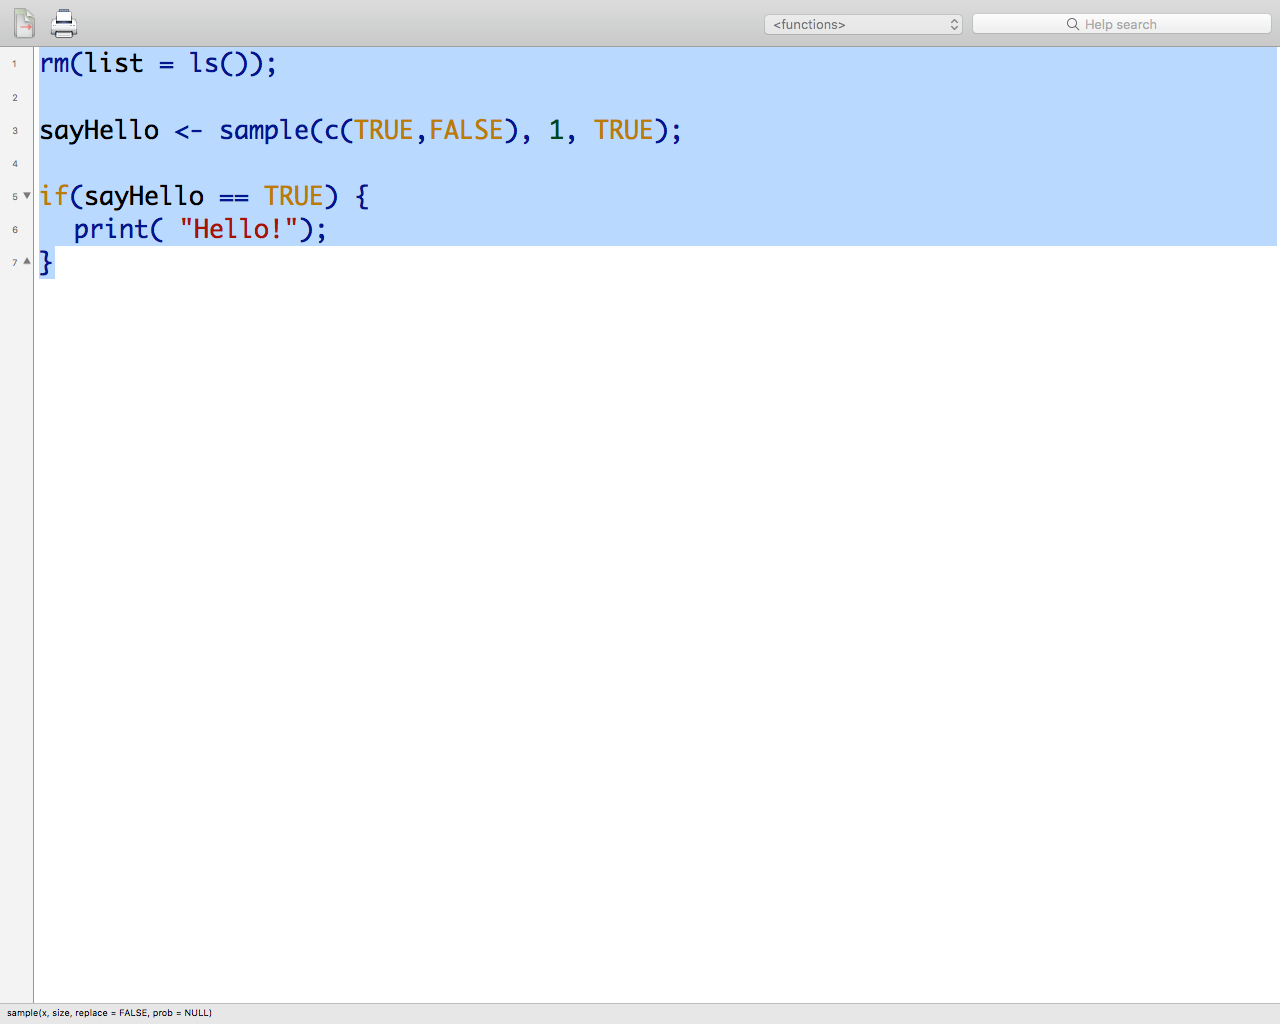
\includegraphics[width=1.0\linewidth]{pic0025}
  \caption{Текстов редактор към продукта R}
\label{figure0025}
\end{figure}
\FloatBarrier

Най-бързият начин за стартиране на скрипта\index{изпълнение на скрипт} е чрез менюто на вградения текстов редактор Edit->Execute (Фиг. \ref{figure0026}). 

\begin{figure}[h!]
  \centering
  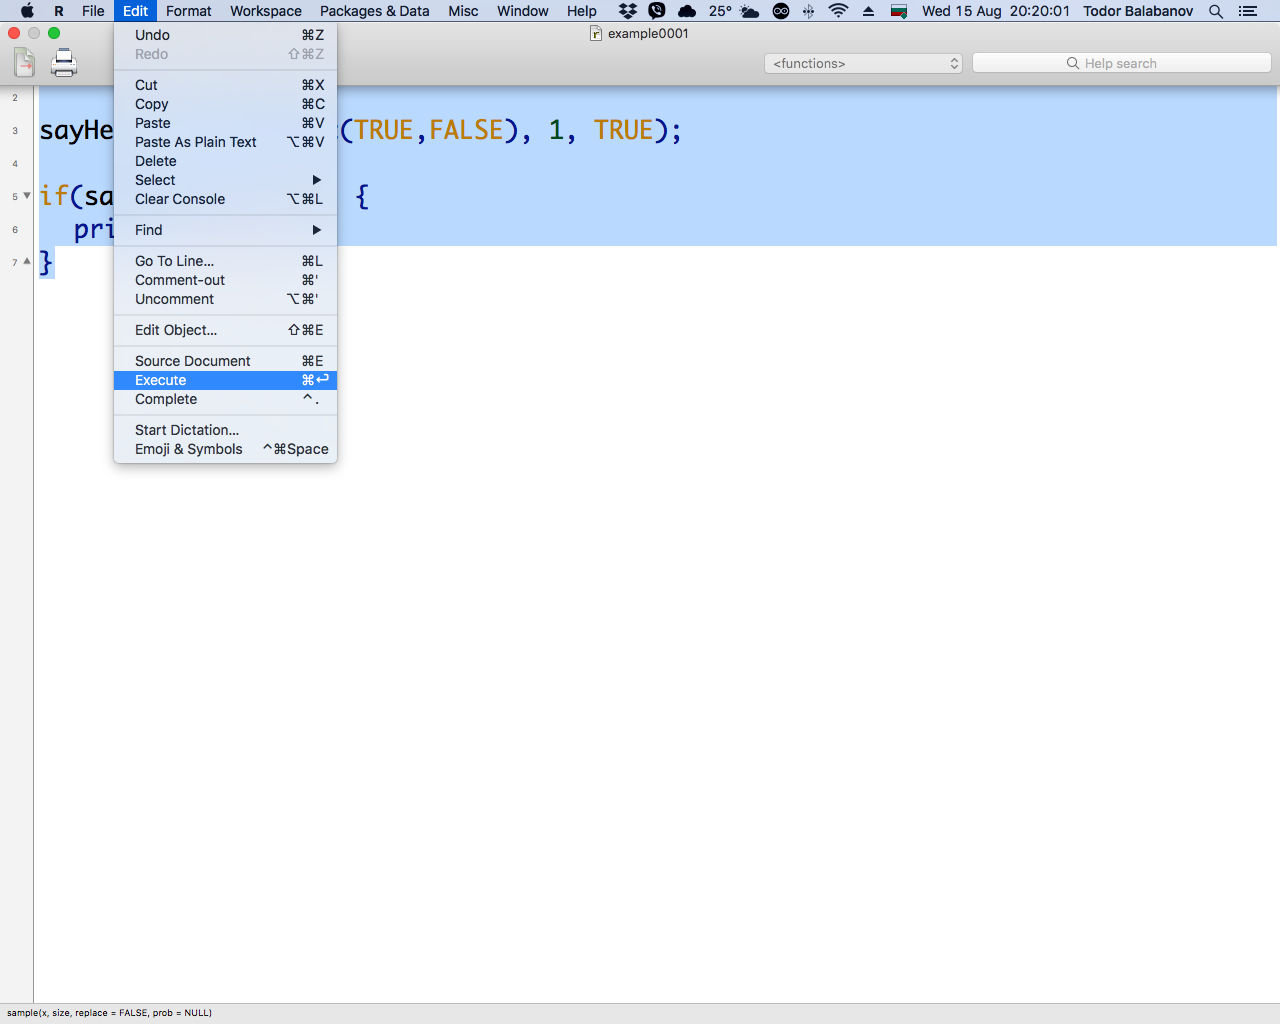
\includegraphics[width=1.0\linewidth]{pic0026}
  \caption{Стартиране на R скрипт}
\label{figure0026}
\end{figure}
\FloatBarrier

Съществено е целият текст на скрипта да бъде маркиран, тъй като командният интерпретатор е оптимизиран в режим за изпълнение на команда по команда. Когато целият скрипт е маркиран се изпълняват, една след друга, всички команди.

\begin{figure}[h!]
  \centering
  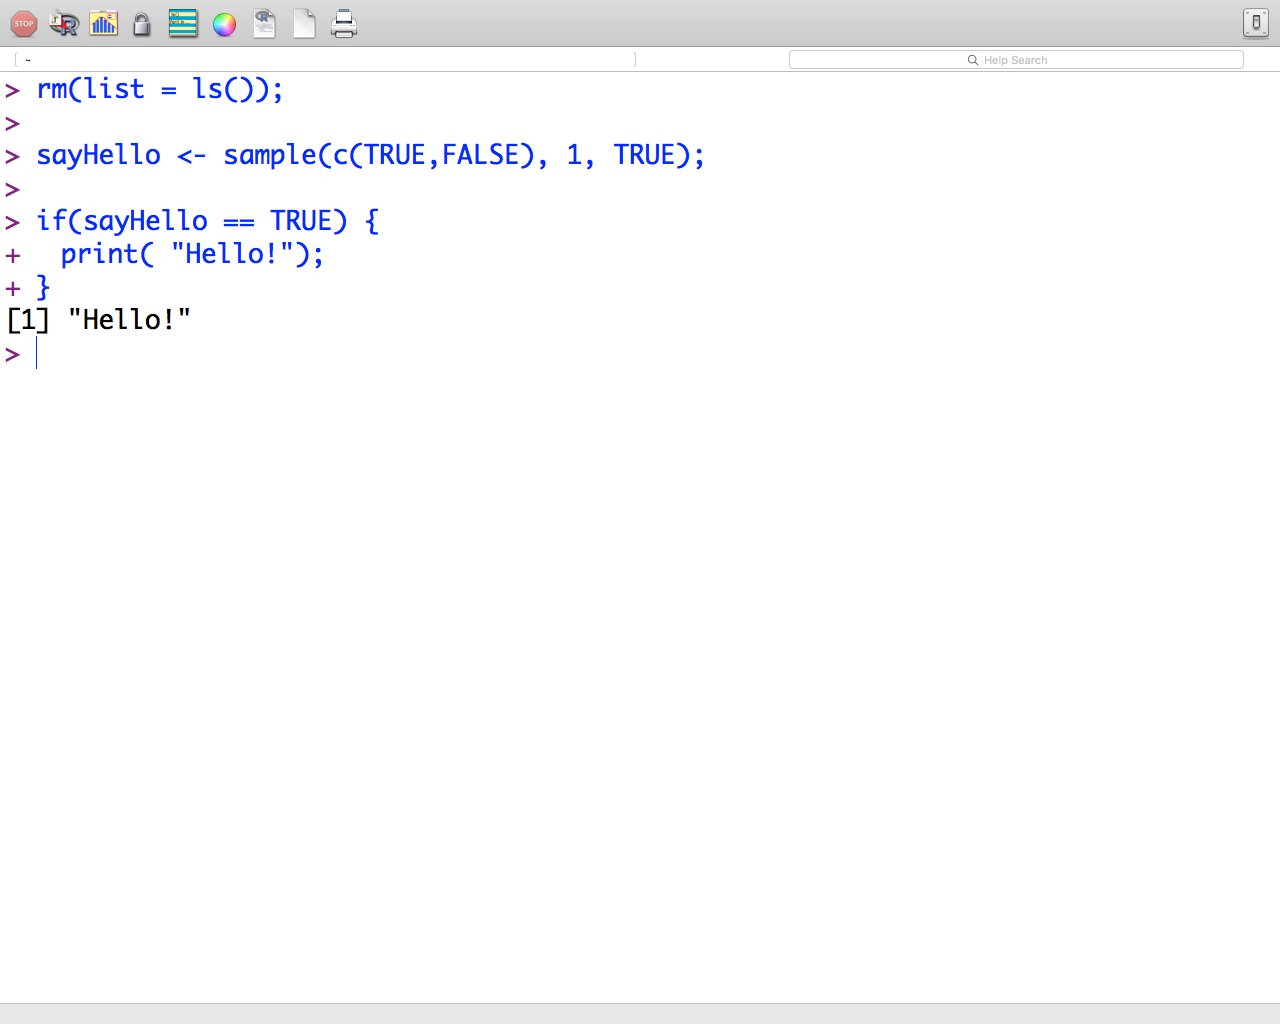
\includegraphics[width=1.0\linewidth]{pic0027}
  \caption{Резултат от изпълнението на R скрипт}
\label{figure0027}
\end{figure}
\FloatBarrier

Резултатът от изпълнението на R скрипта се наблюдава в командния интерпретатор на продукта (Фиг. \ref{figure0027}) и изглежда точно както би трябвало командите да се въведат, на ръка, ако не бяха заредени от скриптов файл.

Алтернативна възможност за стартиране на R скриптове е конзолата на операционната система. При този вариант в конзолата на операционната система се извиква приложението R, а като параметри на приложението се подава файлът съдържащ скрипта и параметър дали сесията от изпълнението на скрипта да бъде съхранена (Листинг \ref{listing0085}).

\begin{lstlisting}[caption=Изпълнение на R скрипт от конзолата на операционната система, label=listing0085]
r < ./Statistical-Data-Processing-with-R/code/example0001.r --no-save
\end{lstlisting}

При такова изпълнение се спестява зареждането на целият програмен продукт R за постоянно в оперативната памет (Фиг. \ref{figure0028}).

\begin{figure}[h!]
  \centering
  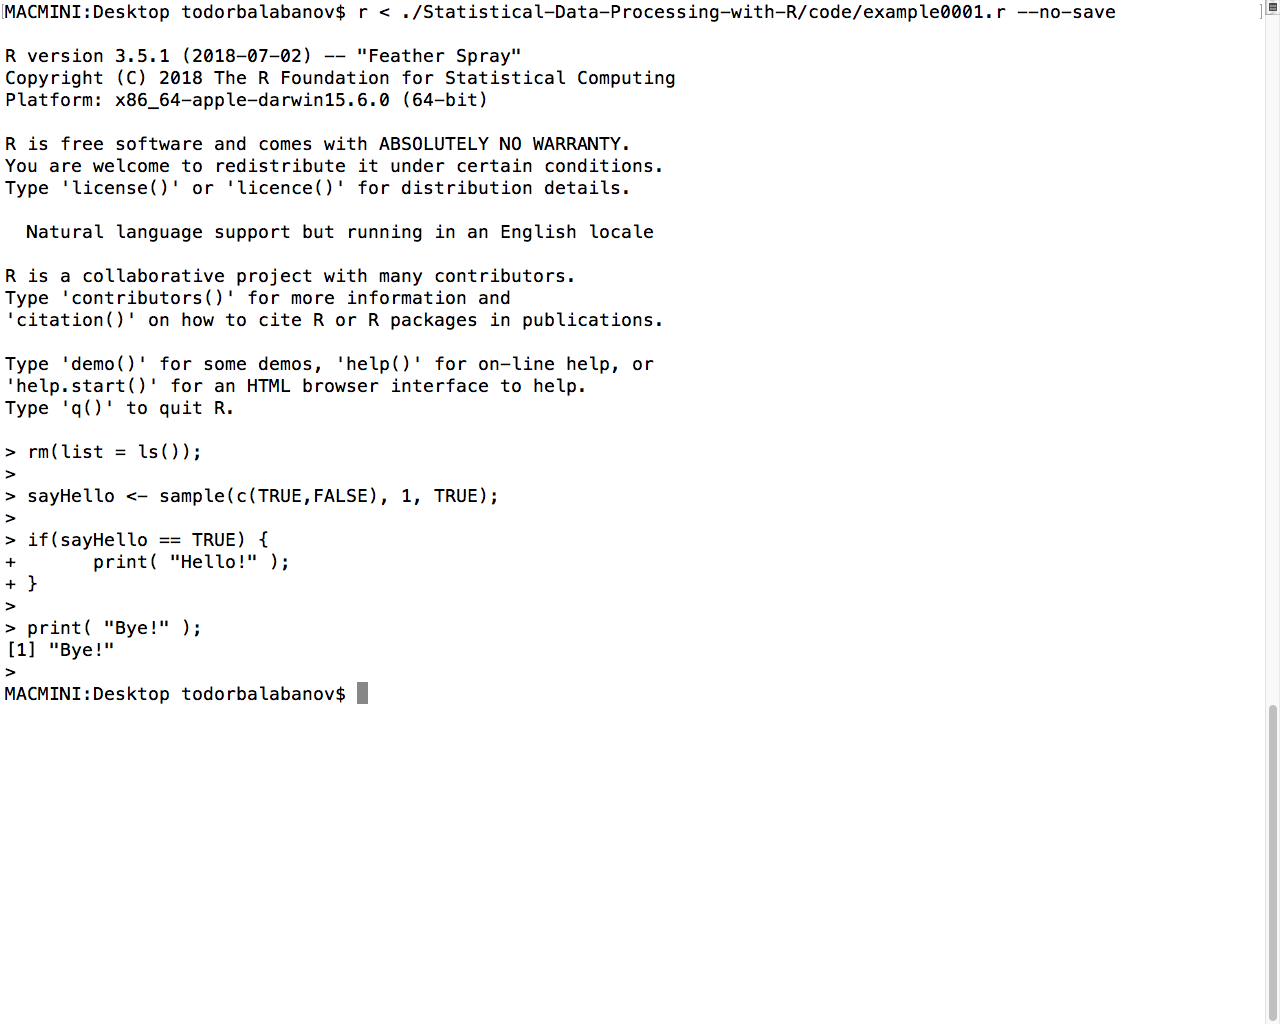
\includegraphics[width=1.0\linewidth]{pic0028}
  \caption{Резултат от изпълнението на R скрипт в конзолата на операционната система}
\label{figure0028}
\end{figure}
\FloatBarrier

Програмните скриптове се състоят от последователни инструкции, но с подходящи оператори за преход или повторение изпълнението на командите може да протече в различен от линейния ред. Тази група оператори се нарича оператори за контрол на изпълнението. Общата конструкция на операторите е заглавна част (ключова дума и условие) и тяло. 

\section{Оператори за преход}

Операторите за условен преход\index{оператори за преход} променят изпълнението на скрипта в зависимост от логическо или числено условие. От там идва и названието им. В тази група оператори попадат if, else и switch.

В заглавните части на операторите за преход може да се проверява само едно условие или да се проверяват цяла група от условия (логически изрази)\index{логически операции}. За тази цел в R има логически операции като „И“ (операции \& и \&\&) и „ИЛИ“ (операции | и ||). При дойната форма на операциите се сравнява само по една стойност от двете страни (не са векторизирани), докато при единичната форма се сравняват елемент по елемент в множества от елементи от двете страни. Поради тази причина двойната форма е полезна при if оператора, а единичната форма се изисква при ifelse конструкцията. Друга много важна разлика между единичната и двойната форма е в начина по който се изчисляват изразите от двете страни на операцията. При единичната форма задължително се изчисляват и двата операнда, независимо дали това действително е нужно. При двойната форма се изчисляват само тези операнди, които са достатъчни за да определят финалният резултат от пресмятането на логическия израз. Тази разлика в използването на логическите операции може да се окаже изключително съществена, когато операндите са функции връщащи логическа стойност. В случаите когато е ненужно някой от операндите да се изчисли, тъй като другите вече са определили резултата, то част от функциите няма да бъдат извикани. С помощта на логическите операции могат да се построят много сложни логически изрази, при които важат общите правила за приоритет на операциите, както и възможността приоритетът да се променя, чрез подходящо поставяне на скоби. 

\subsection{Оператор за условен преход}

Дори чисто исторически в програмните езици един от първите оператори за преход е оператора за условен преход (if оператор)\index{оператор за условен преход}. 

\begin{lstlisting}[caption=Оператор за условен преход if, label=listing0075]
sayHello <- sample(c(TRUE,FALSE), 1, TRUE);

if(sayHello == TRUE) {
	print( "Hello!" );
}

print( "Bye!" );
\end{lstlisting}

Операторът за условен преход използва ключовата дума if (Листинг \ref{listing0075}), а в заглавната му част се записва израз пресмятан до логическа стойност TRUE или FALSE\index{логически стойности}. Смисълът на оператора if е, че тялото му бива изпълнено единствено ако изчислението на израза в заглавната част доведе до стойност TRUE. Ако изразът в заглавната част бъде изчислено до стойност FALSE, тялото на оператора се пропуска и изпълнението на програмата продължава след него.

В примерът от листинг \ref{listing0075} променливата sayHello получава една случайна логическа стойност (TRUE или FALSE), като двете възможности за равно вероятни. На следващият ред операторът if изписва "Hello!" или го пропуска и изписва "Bye!". Скриптът трябва да се стартира няколко пъти за да се наблюдава ефекта от случайния избор на стойност за променливата sayHello.

\subsection{Алтернатива при условен преход}

В множество ситуации, освен основна алтернатива за оператора if, е необходимо да има и допълнителна алтернатива\index{алтернатива при условен преход}, която да се изпълни при резултат от логическия израз FALSE. За тази цел конструкцията на оператора if може да се разшири с добавяне на else конструкция (Листинг \ref{listing0076}).

\begin{lstlisting}[caption=Оператор за условен преход if-else, label=listing0076]
sayHello <- sample(c(TRUE,FALSE), 1, TRUE);

if(sayHello == TRUE) {
	print( "Hello!" );
} else {
	print( "Hi!" );
}

print( "Bye!" );
\end{lstlisting}
Конструкцията else е контекстно зависима и поради тази причина може да се използва единствено в комбинация с конструкцията на оператора if. В примерния код от листинг \ref{listing0076} в половината от случаите на конзолата ще се изпише "Hello!", а в другата половина "Hi!".

\subsection{Каскада от условни преходи}

Условният преход ограничава до две възможности, но практиката понякога налага да се избират повече алтернативи. В такава ситуация може да се използва каскада от if-else конструкции\index{каскада от оператори за условен преход} (Листинг \ref{listing0077}).

\begin{lstlisting}[caption=Каскада от if-else, label=listing0077]
sayHello <- sample(c(0,1,2), 1, TRUE);

if(sayHello == 0) {
	print( "Hello!" );
} else if(sayHello == 1) {
	print( "Hi!" );
} else if(sayHello == 2) {
	print( "Yoo!" );
} else {
	print( "Error!" );
}

print( "Bye!" );
\end{lstlisting}

Недостатък на каскадните проверки е, че всяко условие трябва да бъде проверявано по отделно. Каскадата може да завършва с else конструкция, но тя не е задължителна. 

R предлага ifelse оператор, който много прилича на if конструкцията в Microsoft Excel (Листинг \ref{listing0078}) и сериозно се различава от if-else оператора. Една от най-силните страни на ifelse конструкцията е, че тя е векторизирана и може да се прилага над група елементи едновременно. 

\begin{lstlisting}[caption=Функцията ifelse, label=listing0078]
ifelse(sample(c(FALSE,TRUE), 1, TRUE), "Yes", "No")

ifelse(c(1,1,0,1,0,1)==1, "Yes", "No")
\end{lstlisting}

\subsection{Оператор за многовариантен избор}

Писането на каскадни конструкции от типа if-else може да бъде твърде неудобно и поради тази причина съществува switch конструкцията\index{оператор за многовариантен избор} (Листинг \ref{listing0079}).

\begin{lstlisting}[caption=Конструкция за многовариантен избор switch, label=listing0079]
switch(sample(c("a","b","c","d","e"),1,TRUE), "a"="one", "b"="two", "c"="three", "d"="four", "other")
\end{lstlisting}

В примерния код на случаен принцип се избира една буква от пет възможни, след което се проверяват четири алтернативи и последна опция за else условие. 

Първият аргумент е стойността която ще се проверява, а след това са изброени алтернативните възможности. Последната стойност, ако не й е зададена стойност за проверка, служи за отговор, коато нито една от алтернативите не е била определена. 

\section{Оператори за цикъл}

В конвенционалните програмни езици е обичайна практика елементите на масивите и контейнерите за данни (списъци, стекове, опашки и други) да бъдат обхождани един по един с помощта на цикли. В R целта е да бъдат прилагани векторизирани операции и максимално да се избягва използването на цикли за обхождане на елементи в контейнер за данни. Въпреки това, в някои ситуации се налага използването на цикли\index{оператори за цикъл} и поради тази причина R поддържа циклите for и while. 

\subsection{Цикъл за обхождане}

Операторът for\index{цикъл за обхождане} в R представлява цикъл за обхождане на елементи във вектор, като елементът от текущата итерация е достъпен за използване в тялото на цикъла (Листинг \ref{listing0080}). 

\begin{lstlisting}[caption=Оператор за цикъл for, label=listing0080]
for(number in 1:10) { print(number); }
[1] 1
[1] 2
[1] 3
[1] 4
[1] 5
[1] 6
[1] 7
[1] 8
[1] 9
[1] 10
\end{lstlisting}

Заглавната част се състои от променлива (в случая number), ключовата дума in и вектор от възможни стойности (в случая числата от едно до десет). Векторите могат да бъдат с различен тип на елементите, примерно символни низове (Листинг \ref{listing0081}).

\begin{lstlisting}[caption=Обхождане на вектор от символни низове, label=listing0081]
for(f in c("orange", "lemon", "kiwi", "cherry")) { print(f); }
[1] "orange"
[1] "lemon"
[1] "kiwi"
[1] "cherry"
\end{lstlisting}

\subsection{Цикъл с условие за край}

Когато няма да бъде обхождано множество от елементи е по-удачно да се използва цикълът while\index{цикъл с условие за край}, който в заглавната си част съдържа логически израз, определящ условието за край на цикъла. Цикълът се върти докато логическият израз в заглавната му част се пресмята до стойност TRUE (Листинг \ref{listing0082}). 

\begin{lstlisting}[caption=Цикъл с условие за край, label=listing0082]
counter <- 1;
while(counter <= 5) { 
	print( counter ); 
	counter <- counter + 1;
}
[1] 1
[1] 2
[1] 3
[1] 4
[1] 5
\end{lstlisting}

При цикъла с условие за край, променливата която определя условията за приключване на итереациите трябва да се определи преди началото на цикъла. За да не бъде цикълът безкраен е нужно тази променлива да бъде променена, в тялото на цикъла, по такъв начин, че той да приключи изпълнението си.

\subsection{Прекъсване на циклите}

Понякога се налага определена итерация на цикъла да бъде прекъсната\index{прекъсване на цикли}. За тази цел R предлага ключовата дума next, която прекъсва текущата итерация и преминава към следващата (Листинг \ref{listing0083}).

\begin{lstlisting}[caption=Прекъсване на итерация, label=listing0083]
for(number in 1:10) { 
	if(number == 7) {
		next;
	}

	print(number);
}
[1] 1
[1] 2
[1] 3
[1] 4
[1] 5
[1] 6
[1] 8
[1] 9
[1] 10
\end{lstlisting}

В този случай пропуснатото число е седем, тъй като при седмата итерация е било изпълнено условието на оператора if и неговото тяло съдържа ключовата дума next.

В други ситуации се налага цикълът да бъде спрян изцяло и тогава се използва ключовата дума break (Листинг \ref{listing0084}).

\begin{lstlisting}[caption=Прекъсване на цикъла, label=listing0084]
for(number in 1:10) { 
	if(number == 3) {
		break;
	}

	print(number);
}
[1] 1
[1] 2
\end{lstlisting}

Двете ключови думи (next и break) са контекстно зависими конструкции и могат да се използват единствено в телата на циклите for и while. 

\section{Потребителски функции}

При писането на програмен код в съвременните програмни езици е изключително добра практика кодът да се групира в серия инструкции и те да се оформят като самостоятелна единица. За тази цел, R предлага възможността кодът да се оформя в потребителски написани функции\index{потребителски функции}. 

Оформянето на скриптовете в добре организирани и малки по размер функции е основен похват в съвременното програмиране. Такъв стил на работа позволява по-лесна поддръжка, по-лесна проверка на резултатите създавани от функцията и по-лесна преизползваемост на кода. 

Писането на функции в R малко се различава от повечето конвенционални програмни езици, но много прилича на функциите писани в JavaScript. Самата функция представлява обект, който бива присвоен на идентификатор (Листинг \ref{listing0086}).

\begin{lstlisting}[caption=Примерна потребителска функция, label=listing0086]
say.hello <- function() {
	print("Hello, World!");
}

say.hello();
[1] "Hello, World!"
\end{lstlisting}

Важно е да се отбележи, че символът точка (.) е валиден символ за съставяне на име на функцията. Това е фундаментална разлика спрямо повечето конвенционални програмни езици. Въпреки това, имената не бива да започват само с точка, тъй като обекти именувани по този начин имат по-специфична употреба. Функцията се създава с ключовата дума function\index{дефиниция на функция}, а тялото на функцията се огражда в къдрави скоби. Много добра практика е да се спазват стриктни правила за подравняване на различните конструкции, използвани като команди в тялото на функцията. Такъв стил на писане подобрява възможностите за четене програмния текст и възможностите за откриване на евентуални грешки в него. 

\subsection{Аргументи на функция}

Тъй като функциите са самостоятелно обособени групи от инструкции, то понякога е нужно към групата да бъдат подавани параметри, под формата на аргументи на функцията\index{аргументи на функция} (Листинг \ref{listing0087}). 

\begin{lstlisting}[caption=Извикване на функция с аргумент, label=listing0087]
hello.person <- function( name ) {
	print( sprintf("Hello, %s!",name) );
}

hello.person("Dessislava");
[1] "Hello, Dessislava!"
\end{lstlisting}

Променливата name е достъпна само в тялото на функцията и не може да бъде използвана извън него. 

\begin{lstlisting}[caption=Извикване на функция с повече аргументи, label=listing0088]
hello.person <- function(first, last) {
	print( sprintf("Hello, %s %s!",first,last) );
}

hello.person("Dessislava", "Gruncharova");
[1] "Hello, Dessislava Gruncharova!"

hello.person(last="Mladevnova", first="Vyara");
[1] "Hello, Vyara Mladevnova!"
\end{lstlisting}

Функциите в R позволяват викане с изброяване на параметрите по позиции или чрез явно указване кой аргумент каква стойност да получи (Листинг \ref{listing0088}).

\subsection{Аргументи с подразбираща се стойност}

В някои ситуации е удачно някои от аргументите да имат зададена стойност по подразбиране. В много от съвременните езици това се постига с едноименни функции (overloading), но в R този ефект е възможен, чрез задаване на подразбираща се стойност\index{аргументи на функция с подразбираща се стойност} (Листинг \ref{listing0089}). 

\begin{lstlisting}[caption=Извикване на функция с подразбиращи се аргументи, label=listing0089]
hello.person <- function(first, last, title="") {
	print( sprintf("Hello, %s %s %s!",title,first,last) );
}

hello.person("Zornitsa", "Radeva", "Miss");
[1] "Hello, Miss Zornitsa Radeva!"

hello.person("Todor", "Balabanov");
[1] "Hello,  Todor Balabanov!"
\end{lstlisting}

\subsection{Променлив брой аргументи}

По аналогия с програмния език C, в R са възможни функции с променлив брой аргументи, което се постига с операцията триеточие (...) в заглавната част на функцията (Листинг \ref{listing0090}). Механизмът с променлив брой аргументи\index{функции с променлив брой аргументи} е изключително полезен, но той също така води и до много сериозни програмни грешки. 

\begin{lstlisting}[caption=Функция с променлив брой аргументи, label=listing0090]
sum.up <- function(a, b, ...) {
	print( a+b );
}

sum.up(1, 2, 3, 4);
\end{lstlisting}

\subsection{Върната стойност}

Потребителските функции трябва да се пишат по такъв начин, че да функционират на принципа на черната кутия – аргументи на входа с резултат на изхода и капсулирано изчисление в тялото на функцията. За да бъде постигната тази цел, функциите в R могат да връщат стойност\index{върната стойност от функция}. По аналогия с JavaScript, в R може да се връща стойност от различен тип с ключовата дума return (Листинг \ref{listing0091}).

\begin{lstlisting}[caption=Връщане на стойност от функция, label=listing0091]
sum.up <- function(a, b, ...) {
	return(a + b);
}

print( sum.up(1,2,3,4) );
\end{lstlisting}

\subsection{Предаване на функция като аргумент}

В относително редки случаи се налага върху входните данни да бъдат извикани различни функции. В такава ситуация е важно към самата функция да бъде подаден обект от тип функция\index{функционални обекти} (Листинг \ref{listing0092}).

\begin{lstlisting}[caption=Избор на функция за извикване по време на изпълнение, label=listing0092]
do.stat <- function(values, calculation) {
	do.call(calculation, args=list(values));
}

print( do.stat(1:10,mean) );
[1] 5.5

print( do.stat(1:10,median) );
[1] 5.5

print( do.stat(1:10,sd) );
[1] 3.02765
\end{lstlisting}

В други програмни езици този ефект се постига с функционални указатели (езикът C) или функционални обекти (езикът Java).

\section*{Заключение}

Операторите за контрол на изпълнението позволяват създаването на по-сложни експериментални модели и извършването на по-задълбочени статистически изследвания. За ефективна и надеждна работа, езикът R позволява командите и операторите за контрол на изпълнението да бъдат организирани в отделни потребителски функции и файлове съдържащи програмните скриптове. 


\newpage
\chapter{Групиране и обхождане на данни}
\label{chapter06}

Практиката показва, че около 80\% от статистическия анализ е манипулация на данните. Това често налага повтарящи се операции върху различни участъци от данните. Данните се разделят на отделни фрагменти, след това върху определени фрагменти се прилагат определени операции и накрая фрагментите се обединяват в едно цяло. 

\section{Фамилията функции apply}

Фамилията функции apply служи за групово манипулиране на данни. Тъй като има различни входно-изходни комбинации на данните, то в R е представена цяла фамилия функции, а не една единствена.

\subsection{apply}

Функцията apply е първата, която потребителите научават и тя идва с най-много ограничения. Функцията се прилага върху матрици, което означава че всичките елементи в матрицата трябва да са от един и същи тип. Ако функцията бъде приложена върху друг тип обект, то първо данните ще бъдат преобразувани до матрица. Първият аргумент при извикването е обектът който ще бъде обработван. Вторият аргумент определя дали да се работи по редове (стойност 1) или по колони (стойност 2). Третият аргумент е функцията, която трябва да се приложи. Аргументите след третия могат да са променлив брой и се предават на функцията, която е посочена в третия аргумент. 

\begin{lstlisting}[caption=Сума по редове и колони, label=listing0093]
m1 <- matrix(11:19, nrow=3)
m1
     [,1] [,2] [,3]
[1,]   11   14   17
[2,]   12   15   18
[3,]   13   16   19
 
apply(m1, 1, sum)
[1] 42 45 48
 
apply(m1, 2, sum)
[1] 36 45 54

m1[2,2] <- NA
m1
     [,1] [,2] [,3]
[1,]   11   14   17
[2,]   12   NA   18
[3,]   13   16   19

apply(m1, 1, sum)
[1] 42 NA 48

apply(m1, 2, sum)
[1] 36 NA 54

apply(m1, 1, sum, na.rm=TRUE)
[1] 42 30 48

apply(m1, 2, sum, na.rm=TRUE)
[1] 36 30 54
\end{lstlisting}

Едно от най-лесните пресмятания, за илюстрация на функцията apply, е сумата на елементите по редове и по колони в една матрица (Листинг \ref{listing0093}). Когато в матрицата има неопределени стойност (NA), подадената функция изчислява стойността до NA. Това поведение може да бъде променено, чрез игнориране на липсващите стойности, с подаване на параметъра na.rm=TRUE.

\subsection{lapply и sapply}

Функцията lapply получава като аргумент списък и връща като резултат списък (Листинг \ref{listing0094}). 

\begin{lstlisting}[caption=Сума на обекти в списък, label=listing0094]
l1 <- list(m2=matrix(1:9,3), l2=1:5, m3=matrix(1:4,2), n1=2)
l1
$m2
     [,1] [,2] [,3]
[1,]    1    4    7
[2,]    2    5    8
[3,]    3    6    9

$l2
[1] 1 2 3 4 5

$m3
     [,1] [,2]
[1,]    1    3
[2,]    2    4

$n1
[1] 2

lapply(l1, sum)
$m2
[1] 45

$l2
[1] 15

$m3
[1] 10

$n1
[1] 2

sapply(l1, sum)
m2 l2 m3 n1 
45 15 10  2
\end{lstlisting}

Ако върнатата стойност трябва да бъде вектор, то вместо lapply се използва sapply, която във всяко друго отношение работи като lappy. 

\subsection{mapply}

Функцията mapply се ползва за прилагане на функция върху всеки елемент на от множество списъци (Листинг \ref{listing0095}). 
\begin{lstlisting}[caption=Проверка за идентичност на елементите, label=listing0095]
l3 <- list(m4=matrix(1:25,5), m5=matrix(1:16,2), l4=1:5)
l5 <- list(m6=matrix(1:25,5), m7=matrix(1:16,8), l6=15:1)

mapply(identical, l3, l5)
   m4    m5    l4 
 TRUE FALSE FALSE

mapply(f1<-function(x,y){NROW(x)+NROW(y)}, l3, l5)
m4 m5 l4 
10 10 20 
\end{lstlisting}

Също така, mapply позволява и потребителски дефинирани функции.

\subsection{Агрегация}

При употребата на SQL е много популярно данните да се групират по признак/признаци и върху тях да бъдат изпълнявани агрегатни функции. Един от начините да се постигне агрегация в R е, чрез функцията aggregate и синтаксиса за запис на формула. Формулите се записват с лява част и дясна част, отделени със символа тилда (\textasciitilde). От лявата страна стои променливата по която ще се извършва пресмятането, а от дясната страна стои променлива (или група променливи) по която ще се извършва групирането. 

\begin{lstlisting}[caption=Групиране на данни, label=listing0096]
data(diamonds, package="ggplot2")
head(diamonds, n=3)
  carat     cut color clarity depth table price    x    y    z
1  0.23   Ideal     E     SI2  61.5    55   326 3.95 3.98 2.43
2  0.21 Premium     E     SI1  59.8    61   326 3.89 3.84 2.31
3  0.23    Good     E     VS1  56.9    65   327 4.05 4.07 2.31

aggregate(price~cut, diamonds, mean)
        cut    price
1      Fair 4358.758
2      Good 3928.864
3 Very Good 3981.760
4   Premium 4584.258
5     Ideal 3457.542
\end{lstlisting}

Като пример за групиране и използване на агрегатна функция може да се изпълни пресмятането на средна цена за диамант организирано в групи според вида на среза (Листинг \ref{listing0096}). Първият аргумент на функцията е формулата за групиране, вторият аргумент е обектът с данните, а третия аргумент е функцията, която да се приложи върху отделните групи. Тъй като вторият аргумент показва кое множество данни се използва, то във формулата не е нужно да се оказва множеството, а може да се използват директно имената на колоните. След третия аргумент могат да се добавят и други аргументи, като примерно na.rm=TRUE. 

\begin{lstlisting}[caption=Групиране по повече от една колона, label=listing0097]
aggregate(price~cut+color, diamonds, mean)
         cut color    price
1       Fair     D 4291.061
2       Good     D 3405.382
3  Very Good     D 3470.467
4    Premium     D 3631.293
5      Ideal     D 2629.095
6       Fair     E 3682.312
7       Good     E 3423.644
8  Very Good     E 3214.652
9    Premium     E 3538.914
10     Ideal     E 2597.550
...
\end{lstlisting}

Както в SQL, така и при групирането в R е възможно групирането да се извърши по повече от една колона (Листинг \ref{listing0097}).

\begin{lstlisting}[caption=Прилагане на агрегатна функция върху повече колони в едни и същи групи, label=listing0098]
aggregate(cbind(price,carat)~cut, diamonds, mean)
        cut    price     carat
1      Fair 4358.758 1.0461366
2      Good 3928.864 0.8491847
3 Very Good 3981.760 0.8063814
4   Premium 4584.258 0.8919549
5     Ideal 3457.542 0.7028370
\end{lstlisting}

Възможно е агрегатната функция да бъде приложена върху повече от една колона, като това се постига с функцията cbind (Листинг \ref{listing0098}). Особеността при това извикване е, че само една агрегатна функция може да се приложи и всички избрани колони ще бъдат пресметнати спрямо нея (в случая се изчислява средна стойност).

\begin{lstlisting}[caption=Използване на повече колони от двете страни на формулата, label=listing0099]
aggregate(cbind(price,carat)~cut+color, diamonds, mean)
         cut color    price     carat
1       Fair     D 4291.061 0.9201227
2       Good     D 3405.382 0.7445166
3  Very Good     D 3470.467 0.6964243
4    Premium     D 3631.293 0.7215471
5      Ideal     D 2629.095 0.5657657
6       Fair     E 3682.312 0.8566071
7       Good     E 3423.644 0.7451340
8  Very Good     E 3214.652 0.6763167
9    Premium     E 3538.914 0.7177450
10     Ideal     E 2597.550 0.5784012
...
\end{lstlisting}

Изпълнението на агрегатни функции позволява да има повече от една колона и от двете страни на формулата (Листинг \ref{listing0099}). При използването на функцията за агрегация трябва да се има предвид, че тя може да бъде много бавна по отношение на изпълнението, особено при данни с голям обем. 

\section{Пакетът plyr}

Пакетът plyr дава допълнителни възможности по схемата за обработка на данни разделяне-манипулиране-обединение. Ядрото на пакета се състои от функциите ddply, llply и ldply. При тези функции е използвана конвенция, която подсказва какъв е типът на входните данни и типът на изходните данни (в по-широката й употреба това е унгарската нотация \cite{hnot}). Първата буква определя входния тип данни, а втората буква определя изходния тип данни. Буквата d се използва за data.frame, буквата l за списък, буквата a за масив и символът за подчертаване (\_) при липса на върната стойност. 

\subsection{ddply}

За илюстрация на функцията ddply е удачно да се използват данните за бейзболни резултати от пакета plyr (Листинг \ref{listing0100}).

\begin{lstlisting}[caption=Бейзболна статистика, label=listing0100]
library( plyr )

head(baseball,n=3)
          id year stint team lg  g  ab  r  h X2b X3b hr rbi sb cs bb so ibb
4  ansonca01 1871     1  RC1    25 120 29 39  11   3  0  16  6  2  2  1  NA
44 forceda01 1871     1  WS3    32 162 45 45   9   4  0  29  8  0  4  0  NA
68 mathebo01 1871     1  FW1    19  89 15 24   3   1  0  10  2  1  2  0  NA
   hbp sh sf gidp
4   NA NA NA   NA
44  NA NA NA   NA
68  NA NA NA   NA
\end{lstlisting}

В това множество данни са отчетени 21699 записа в бейзболната статистика за 1228 играча, в диапазона от годините 1871 до 2007. Включени са само играчи с 15 или повече сезона игра. В множеството се отчитат 22 признака (колони), със следното значение:

\begin{table}[h!]
\centering
\begin{tabular}{|l|r|} 
  \rowcolor{lightgray}
  \hline
  Характеристика & Значение \\ [0.1ex] 
  \hline\hline
  id & Идентификатор на играча (символен низ) \\
  \hline
  year & Година на събраните данни (цяло число) \\
  \hline
  stint & Ограничения (цяло число) \\
  \hline
  team & Отбор в който играе (символен низ) \\
  \hline
  lg & Лига в която играе (символен низ) \\
  \hline
  g & Брой игри (цяло число) \\
  \hline
  ab & Брой батирания (цяло число) \\
  \hline
  r & Брой пробягвания (цяло число) \\
  \hline
  h & Брой реализирани удари (цяло число) \\
  \hline
  X2b & Брой успешни достигания до втора база (цяло число) \\
  \hline
  X3b & Брой успешни достигания до трета база (цяло число) \\
  \hline
  hr & Брой успешни хум ръна (цяло число) \\
  \hline
  rbi & Брой тичания в които е удрял (цяло число) \\
  \hline
  sb & Брой откраднати бази (цяло число) \\
  \hline
  cs & Брой хванати отнемания (цяло число) \\
  \hline
  bb & Брой пробягвания (цяло число) \\
  \hline
  so & Брой изхвърлени изстрели (цяло число) \\
  \hline
  ibb & Брой международни пробягвания (цяло число) \\
  \hline
  hbp & Брой попадения от питчъра (цяло число) \\
  \hline
  sh & Брой пожертвани удари (цяло число) \\
  \hline
  sf & Брой пожертвани изстрела (цяло число) \\
  \hline
  gidp & Брой приземявания при двойна игра (цяло число) \\
  \hline
\end{tabular}
\caption{Характеристики на бейзболните играчи}
\label{table0003}
\end{table}

Основна статистика в бейзбола е OBP (On Base Percentage), която се изчислява по формула \ref{equation0001}.

\begin{equation}
OBP = \frac{H + BB + HBP}{AB + BB + HBP + SF}
\label{equation0001}
\end{equation}
\listofequations{On Base Percentage (OBP) статистика}

Където:
H – брой удари,
BB – пробягвания,
HBP – брой попадения от питчъра,
AB – удари на батата,
SF – пропуснати изстрели.

Преди 1954 година, за SF стойностите са 0, поради различния начин за отчитане на статистиката. В данните има множество NA стойности за HBP. Липсващите стойности трябва да се заменят с 0. От множеството данни се изключват и всички редове за които AB е по-малко от 50 (Листинг \ref{listing0101}).

\begin{lstlisting}[caption=Корекция на данните, label=listing0101]
any( is.na(baseball$sf) )
[1] TRUE

baseball$sf[baseball$year < 1954] <- 0

any( is.na(baseball$sf) )
[1] FALSE

any( is.na(baseball$hbp) )
[1] TRUE
 
baseball$hbp[ is.na(baseball$hbp) ] <- 0
 
any( is.na(baseball$hbp) )
[1] FALSE

baseball <- baseball[baseball$ab>=50,]
\end{lstlisting}

Пресмятането на OBP коефициентът за всеки играч, за конкретна година е изключително лесно поради възможността да се изпълни векторно пресмятане (Листинг \ref{listing0102}).

\begin{lstlisting}[caption=Пресмятане на OBP, label=listing0102]
baseball$OBP <- with(baseball, (h+bb+hbp)/(ab+bb+hbp+sf))

head(cbind(baseball$id,baseball$OBP), n=3)
     [,1]        [,2]               
[1,] "ansonca01" "0.336065573770492"
[2,] "forceda01" "0.295180722891566"
[3,] "mathebo01" "0.285714285714286"
\end{lstlisting}


Функцията with позволява да се упомене обекта с данните само един път, а в следващите аргументи да се използват само имената на колоните, без да се уточнява на кое множество данни принадлежат. 

OBP коефициента за цялата кариера на играча не може да се пресметне чрез просто усредняване на сезонния OBP коефициент. Трябва да се пресметне и сумира числителят и след това да се раздели на сумата в делителя. Това може да се постигне с функцията ddply (Листинг \ref{listing0103}).

\begin{lstlisting}[caption=Пресмятане на OBP за цялата кариера на играча, label=listing0103]
career <- ddply(baseball, .variables="id", .fun=function(data){c(OBP=with(data,sum(h+bb+hbp)/sum(ab+bb+hbp+sf)))})

career <- career[order(career$OBP,decreasing=TRUE), ]

head(career, n=3)
            id       OBP
1089 willite01 0.4816861
875   ruthba01 0.4742209
658  mcgrajo01 0.4657478
\end{lstlisting}

Вградената потребителска функция извършва пресмятането, а след това ddply изпълнява пресмятането върху всеки играч. Полученият резултат е сортиран в нисходящ ред, според кариерния OBP коефициент.

\subsection{llply}

Функцията llply може да бъде използвана по аналогичен начин както се използва функцията lapply (Листинг \ref{listing0104}).

\begin{lstlisting}[caption=Сума на всеки елемент в списък, label=listing0104]
l1 <- list(m2=matrix(1:9,3), l2=1:5, m3=matrix(1:4,2), n1=2)

llply(l1, sum)
$m2
[1] 45

$l2
[1] 15

$m3
[1] 10

$n1
[1] 2

identical(lapply(l1,sum), llply(l1,sum))
[1] TRUE

laply(l1, sum)
[1] 45 15 10  2
\end{lstlisting}

Функцията laply извършва същото пресмятане, но връща резултата под формата на вектор. 

\subsection{Помощни функции и бързодействие}

В пакета plyr са добавени група помощни функции, като функцията each, която позволява да се изпращат повече от една агрегатна функция на функцията aggregate (Листинг \ref{listing0105}). Недостатък на each е, че тя отнема възможността за изпращане на допълнителни параметри. 

\begin{lstlisting}[caption=Повече от една агрегатни функции, label=listing0105]
library(ggplot2)

aggregate(price~cut, diamonds, each(mean, median))
        cut price.mean price.median
1      Fair   4358.758     3282.000
2      Good   3928.864     3050.500
3 Very Good   3981.760     2648.000
4   Premium   4584.258     3185.000
5     Ideal   3457.542     1810.000
\end{lstlisting}

Друга полезна функция е idata.frame, която позволява създаването на референция към data.frame, така че формирането на подмножества да става по-бързо и при значително по-ниска консумация на оперативна памет (Листинг \ref{listing0106}). 

\begin{lstlisting}[caption=Бързодействие при използване на референции, label=listing0106]
system.time(dlply(baseball, "id", nrow))
   user  system elapsed 
  0.159   0.009   0.169 

reference <- idata.frame( baseball )

system.time(dlply(reference, "id", nrow))
   user  system elapsed 
  0.178   0.005   0.183
\end{lstlisting}

Ускорението което ще се постигне много зависи от размера на данните и от вида на пресмятането, което се извършва над тях. Пакетът plyr често води до компромис с бързодействието в замяна на по-голямо удобство при пресмятането. Повечето функции в пакета може да се изпълнят и с функции от базовата инсталация, plyr просто дава по-удобен начин за пресмятане. 

\section{Пакетът data.table}

Този пакет е създаден с идеята да увеличи възможностите за използване на data.frame структурата от данни. Пакетът изисква малко по-различен синтаксис за работа, спрямо този който вече е наложен при използването на data.frame. Бързодействието при data.table основно се дължи на това, че вътрешната реализация е аналогична на индексите при базите данни. Това позволява по-бърз достъп до данните, по-бързи операции за групиране и по-бързи операции за сливане (join). 

\begin{lstlisting}[caption=Създаване на data.table, label=listing0107]
library(data.table)

df <- data.frame(x1=10:1, x2=letters[11:20], x3=LETTERS[1:10], x4=rep(c("One", "Two", "Three"), length.out=10))
 
df
   x1 x2 x3    x4
1  10  k  A   One
2   9  l  B   Two
3   8  m  C Three
4   7  n  D   One
5   6  o  E   Two
6   5  p  F Three
7   4  q  G   One
8   3  r  H   Two
9   2  s  I Three
10  1  t  J   One

class( df$x2 )
[1] "factor"

dt <- data.table(x1=10:1, x2=letters[11:20], x3=LETTERS[1:10], x4=rep(c("One", "Two", "Three"), length.out=10))
 
dt
    x1 x2 x3    x4
 1: 10  k  A   One
 2:  9  l  B   Two
 3:  8  m  C Three
 4:  7  n  D   One
 5:  6  o  E   Two
 6:  5  p  F Three
 7:  4  q  G   One
 8:  3  r  H   Two
 9:  2  s  I Three
10:  1  t  J   One

class( dt$x2 )
[1] "character"
\end{lstlisting}

Създаването на data.table не се различава особено от създаването на data.frame (Листинг \ref{listing0107}). Зареждането на данни е идентично с разликата, че data.frame преобразува символните низове до фактори, докато data.table ги запазва, като символни низове. 

\begin{lstlisting}[caption=Зареждане на data.table от data.frame, label=listing0108]
diamonds <- data.table(diamonds)

diamonds
       carat       cut color clarity depth table price    x    y    z
    1:  0.23     Ideal     E     SI2  61.5    55   326 3.95 3.98 2.43
    2:  0.21   Premium     E     SI1  59.8    61   326 3.89 3.84 2.31
    3:  0.23      Good     E     VS1  56.9    65   327 4.05 4.07 2.31
    4:  0.29   Premium     I     VS2  62.4    58   334 4.20 4.23 2.63
    5:  0.31      Good     J     SI2  63.3    58   335 4.34 4.35 2.75
   ---                                                               
53936:  0.72     Ideal     D     SI1  60.8    57  2757 5.75 5.76 3.50
53937:  0.72      Good     D     SI1  63.1    55  2757 5.69 5.75 3.61
53938:  0.70 Very Good     D     SI1  62.8    60  2757 5.66 5.68 3.56
53939:  0.86   Premium     H     SI2  61.0    58  2757 6.15 6.12 3.74
53940:  0.75     Ideal     D     SI2  62.2    55  2757 5.83 5.87 3.64
\end{lstlisting}

Създаването на data.table от data.frame става, чрез просто извикване на функцията (Листинг \ref{listing0108}). При разпечатването на резултата има разлика в това, че се показват първите пет и последните пет реда от данните. 

\begin{lstlisting}[caption=Достъп до редовете, label=listing0109]
dt[1:2, ]
   x1 x2 x3  x4
1: 10  k  A One
2:  9  l  B Two

dt[dt$x1>=7, ]
   x1 x2 x3    x4
1: 10  k  A   One
2:  9  l  B   Two
3:  8  m  C Three
4:  7  n  D   One

dt[x1>=7, ]
   x1 x2 x3    x4
1: 10  k  A   One
2:  9  l  B   Two
3:  8  m  C Three
4:  7  n  D   One
\end{lstlisting}

Достъпът до редовете се осъществява по аналогичен начин, както е при data.frame (Листинг \ref{listing0109}). Третото позоваване е възможно, тъй като data.table знае как да открие нужната колона и без да е указана точната data.table променлива. 

\begin{lstlisting}[caption=Достъп до колоните, label=listing0110]
dt[,list(x3,x4)]
    x3    x4
 1:  A   One
 2:  B   Two
 3:  C Three
 4:  D   One
 5:  E   Two
 6:  F Three
 7:  G   One
 8:  H   Two
 9:  I Three
10:  J   One

dt[, x1]
 [1] 10  9  8  7  6  5  4  3  2  1

dt[,list(x2)]
    x2
 1:  k
 2:  l
 3:  m
 4:  n
 5:  o
 6:  p
 7:  q
 8:  r
 9:  s
10:  t

dt[, "x4", with=FALSE]
       x4
 1:   One
 2:   Two
 3: Three
 4:   One
 5:   Two
 6: Three
 7:   One
 8:   Two
 9: Three
10:   One

td[, c("x2", "x3"), with=FALSE]
    x2 x3
 1:  k  A
 2:  l  B
 3:  m  C
 4:  n  D
 5:  o  E
 6:  p  F
 7:  q  G
 8:  r  H
 9:  s  I
10:  t  J
\end{lstlisting}

Достъпът до колоните се осъществява малко по-различно спрямо data.frame (Листинг \ref{listing0110}). За да се позоват колоните като символни низове (примерно получени след някакво пресмятане) трябва да се подаде лъжа на параметъра with. 

\subsection{Ключове}

При наличие на няколко таблици в паметта, то с тях може да се изпълнят серия операции. Като начало, списък с наличните таблици може да се получи чрез функцията tables (Листинг \ref{listing0111}).

\begin{lstlisting}[caption=Операции с таблици, label=listing0111]
tables()
       NAME   NROW NCOL MB                                    COLS KEY
1: diamonds 53,940   10  3 carat,cut,color,clarity,depth,table,...    
2:       dt     10    4  0                             x1,x2,x3,x4    
Total: 3MB

setkey(dt, x4)

dt
    x1 x2 x3    x4
 1: 10  k  A   One
 2:  7  n  D   One
 3:  4  q  G   One
 4:  1  t  J   One
 5:  8  m  C Three
 6:  5  p  F Three
 7:  2  s  I Three
 8:  9  l  B   Two
 9:  6  o  E   Two
10:  3  r  H   Two

tables()
       NAME   NROW NCOL MB                                    COLS KEY
1: diamonds 53,940   10  3 carat,cut,color,clarity,depth,table,...    
2:       dt     10    4  0                             x1,x2,x3,x4  x4
Total: 3MB

key( dt )
[1] "x4"

dt["One", ]
   x1 x2 x3  x4
1: 10  k  A One
2:  7  n  D One
3:  4  q  G One
4:  1  t  J One

dt[c("One","Two"), ]
   x1 x2 x3  x4
1: 10  k  A One
2:  7  n  D One
3:  4  q  G One
4:  1  t  J One
5:  9  l  B Two
6:  6  o  E Two
7:  3  r  H Two

setkey(diamonds, cut, color)

diamonds
       carat   cut color clarity depth table price    x    y    z
    1:  0.75  Fair     D     SI2  64.6    57  2848 5.74 5.72 3.70
    2:  0.71  Fair     D     VS2  56.9    65  2858 5.89 5.84 3.34
    3:  0.90  Fair     D     SI2  66.9    57  2885 6.02 5.90 3.99
    4:  1.00  Fair     D     SI2  69.3    58  2974 5.96 5.87 4.10
    5:  1.01  Fair     D     SI2  64.6    56  3003 6.31 6.24 4.05
   ---                                                           
53936:  0.71 Ideal     J     SI1  60.6    57  2700 5.78 5.83 3.52
53937:  0.81 Ideal     J     VS2  62.1    56  2708 5.92 5.97 3.69
53938:  0.84 Ideal     J     VS2  61.1    57  2709 6.09 6.12 3.73
53939:  0.82 Ideal     J     VS2  61.6    56  2741 6.00 6.04 3.71
53940:  0.83 Ideal     J     VS2  62.3    55  2742 6.01 6.03 3.75

diamonds[J("Fair", "J"), ]
     carat  cut color clarity depth table price    x    y    z
  1:  1.05 Fair     J     SI2  65.8    59  2789 6.41 6.27 4.18
  2:  1.00 Fair     J     VS2  65.7    59  2811 6.14 6.07 4.01
  3:  0.99 Fair     J     SI1  55.0    61  2812 6.72 6.67 3.68
  4:  0.90 Fair     J     VS2  65.0    56  2815 6.08 6.04 3.94
  5:  0.91 Fair     J     VS2  64.4    62  2854 6.06 6.03 3.89
 ---                                                          
115:  0.90 Fair     J     SI1  64.6    61  2438 5.92 5.87 3.81
116:  0.96 Fair     J     SI1  67.3    56  2517 6.06 6.01 4.06
117:  0.90 Fair     J     SI2  66.6    54  2536 6.05 5.99 4.01
118:  0.97 Fair     J     SI2  60.8    67  2538 6.41 6.32 3.87
119:  1.01 Fair     J     SI2  66.9    58  2683 6.13 6.07 4.08
\end{lstlisting}

Както се вижда, нито една от таблиците няма присвоен ключ. Ключът е индексирана колона, която дава допълнително бързодействие при извършването на някои операции. При наличие на ключово поле е възможно изборът на редове да става и чрез подаване на стойности от ключовото поле. Ключът може да бъде и съставен, ако съдържа повече от едно поле. С функцията J служи за достъп до редовете според стойности на съставния ключ. 

\subsection{Агрегация}

Основното предимство на индексираните данни е бързодействието при изпълнението на агрегатни функции. Въпреки че aggregate и фамилията функции d*ply работят с data.table обекти (Листинг \ref{listing0112}), то използването им е свързано с бавно изпълнение. 

\begin{lstlisting}[caption=Агрегатни функции, label=listing0112]
aggregate(price~cut, diamonds, mean)
        cut    price
1      Fair 4358.758
2      Good 3928.864
3 Very Good 3981.760
4   Premium 4584.258
5     Ideal 3457.542

diamonds[, list(price=mean(price)), by=cut]
         cut    price
1:      Fair 4358.758
2:      Good 3928.864
3: Very Good 3981.760
4:   Premium 4584.258
5:     Ideal 3457.542

diamonds[, list(price=mean(price)), by=list(cut,color)]
          cut color    price
 1:      Fair     D 4291.061
 2:      Fair     E 3682.312
 3:      Fair     F 3827.003
 4:      Fair     G 4239.255
 5:      Fair     H 5135.683
 6:      Fair     I 4685.446
 7:      Fair     J 4975.655
...
29:     Ideal     D 2629.095
30:     Ideal     E 2597.550
31:     Ideal     F 3374.939
32:     Ideal     G 3720.706
33:     Ideal     H 3889.335
34:     Ideal     I 4451.970
35:     Ideal     J 4918.186
          cut color    price

diamonds[, list(price=mean(price),carat=sum(carat)), by=list(cut,color)]
          cut color    price   carat
 1:      Fair     D 4291.061  149.98
 2:      Fair     E 3682.312  191.88
 3:      Fair     F 3827.003  282.27
 4:      Fair     G 4239.255  321.48
 5:      Fair     H 5135.683  369.41
 6:      Fair     I 4685.446  209.66
 7:      Fair     J 4975.655  159.60
...
29:     Ideal     D 2629.095 1603.38
30:     Ideal     E 2597.550 2257.50
31:     Ideal     F 3374.939 2509.20
32:     Ideal     G 3720.706 3422.29
33:     Ideal     H 3889.335 2490.52
34:     Ideal     I 4451.970 1910.97
35:     Ideal     J 4918.186  952.98
          cut color    price   carat
\end{lstlisting}

По-добрият вариант е да се използват вградените в data.table агрегатни функции. За да бъде агрегацията по повече от една колона, то нужните колони се подават като списък. За разлика от предишната агрегация, тук могат да се подават различни агрегатни функции (средна и сума, в показания пример), както и да се ползват списък от колони за групиране и за агрегиране. 

\section{Бързи операции с пакета dplyr}

Пакетът dplyr е създаден основно с идеята за ускорение на изпълнението, спрямо бързодействието постигнато в пакета plyr. Пакетът dplyr основно борави с обекти от тип data.frame, а за списъци и вектори е предназначен пакетът purrr. Характерно за dplyr е, че използва названия на някои от функциите, които са добре познати в езика SQL. 

Когато се работи едновременно с пакетите plyr и dplyr е важен редът на зареждането им, тъй като последно заредения пакет в R е с приоритет, при наличие на едноименни функции. При колизия на имената конфликтът се разрешава чрез операцията за принадлежност към пакет (::), като от лявата страна е името на пакета, а от дясната страна името на функцията. Пример за такава колизия е функцията за обобщение на данните в двата пакета - plyr::summarize и dplyr::summarize.

\subsection{Потоци и таблици}

Концепцията за потоците (pipes) е развита още с първите масово използвани операционни системи, а в езика R тя е възможна благодарение на пакета magrittr. При класическата работа с функции, резултатът от извикването на първата функция се записва в междинна променлива, тази променлива се подава като аргумент на втората функция, която на свой ред записва във втора междинна променлива и този процес може да се повтаря многократно. Потоците позволяват да се избегне използването на междинни променливи, а използването на функциите да се организира като една верига от извиквания (Листинг \ref{listing0113}). Синтаксисът за поточна операция в R е два символа за процент и знакът за по-голямо между тях (\%>\%).

\begin{lstlisting}[caption=Поточни операции, label=listing0113]
library( ggplot2 )
library( magrittr )
 
dim( head(diamonds,n=4) )
[1]  4 10
 
diamonds %>% head(4) %>% dim
[1]  4 10
\end{lstlisting}

С поточната операция се подава обекта, като първи аргумент на съответната функция. Поточните операции могат да се навързват във верига и обектът в резултат от изпълнението на една функция да се предава към следваща. 

По аналогия с обектите от тип data.table, пакетът dplyr предлага разширение на data.frame под формата на tbl обекти, които се доразвиват и в пакета tibble. Съществено за tbl е, че при разпечатване се показват само подмножество на редовете, но също и подмножество на колоните, докато бъде изпълнен екрана. Третата разлика е, че под имената на колоните се визуализира информация за типът данни в колоната. При по-новите реализации на пакета ggplot2, данните за диамантите са представени и като tbl обект (Листинг \ref{listing0114}).

\begin{lstlisting}[caption=Таблични данни в dplyr, label=listing0114]
class( diamonds )
[1] "tbl_df"     "tbl"        "data.frame"

head(diamonds, n=3)
# A tibble: 3 x 10
  carat cut     color clarity depth table price     x     y     z
  <dbl> <ord>   <ord> <ord>   <dbl> <dbl> <int> <dbl> <dbl> <dbl>
1  0.23 Ideal   E     SI2      61.5    55   326  3.95  3.98  2.43
2  0.21 Premium E     SI1      59.8    61   326  3.89  3.84  2.31
3  0.23 Good    E     VS1      56.9    65   327  4.05  4.07  2.31
\end{lstlisting}

\subsection{Извличане по колони}

По аналогия с SQL, функцията select извършва подбор на редове от зададено множество данни (Листинг \ref{listing0115}). Първият аргумент е data.frame (или tbl обект), а следващите аргументи изброяват желаните колони. Функцията може да се използва самостоятелно или с потоци.

\begin{lstlisting}[caption=Избор на редове, label=listing0115]
library( dplyr )

select(diamonds, carat, price)
diamonds %>% select(carat, price)
diamonds %>% select(c(carat, price))

diamonds %>% select_('carat', 'price')
names <- c('carat', 'price')
diamonds %>% select_(.dots=names)

diamonds %>% select( one_of('carat', 'price') )
names <- c('carat', 'price')
diamonds %>% select( one_of(names) )

select(diamonds, 1, 7)
diamonds %>% select(1, 7)
\end{lstlisting}

Функцията select позволява извикване по множество различни начини, които могат да доведат до един и същи начин. Като аргументи, select получава директно имената на колоните, без те да са обградени в кавички (тоест не са символни низове). Когато е нужно имената на колоните да се подават като символни низове се използва функцията select\_, която се различава в името си с една подчертавка в края. Ако имената на колоните са запазени в променлива то те се подават на .dots параметъра. От версия 0.6.0 на пакета dplyr не се препоръчва използването на функцията select\_, а заместването й с функцията select и аргумент върнат, като стойност от функцията one\_of. На функцията select освен имена на колони, може да се подават и техните индекси. 

\begin{lstlisting}[caption=Търсене по частично съвпадение, label=listing0116]
diamonds %>% select( starts_with('c') )
diamonds %>% select( ends_with('e') )
diamonds %>% select( contains('l') )

diamonds %>% select( matches('r.+t') )
\end{lstlisting}

Понякога в практиката се налага подбор на колони в множеството от данни по критерии за частично съвпадение (Листинг \ref{listing0116}). При такава ситуация за начало се ползва функцията starts\_with, за край функцията ends\_with, а за съдържание функцията contains. При частичния избор е възможно да с използват и ретуларни изрази. 

\begin{lstlisting}[caption=Изключване на колони, label=listing0117]
diamonds %>% select(-carat, -price)
diamonds %>% select( -c(carat, price) )
diamonds %>% select(-1, -7)
diamonds %>% select( -c(1,7) )
diamonds %>% select_(.dots=c('-carat', '-price'))
diamonds %>% select( -one_of('carat','price') )
\end{lstlisting}

В някои ситуации от множеството колони трябва да се изключат една част. Това се постига със записване на знак минус пред името/имената на колоната/колоните (Листинг \ref{listing0117}).

\subsection{Филтриране}

Филтрирането се състои в избиране на редове от данните по зададен критерии (логически израз). 

\begin{lstlisting}[caption=Филтриране на редове, label=listing0118]
library( ggplot2 )
library( magrittr )
library( dplyr )

diamonds %>% filter(cut == 'Ideal')
diamonds[diamonds$cut == 'Ideal', ]

diamonds %>% filter(cut %in% c('Ideal', 'Good'))

diamonds %>% filter(carat > 2, price < 14000)
diamonds %>% filter(carat > 2 & price < 14000)

diamonds %>% filter(carat < 1 | carat > 5)

diamonds %>% filter_("cut == 'Ideal'")
diamonds %>% filter_(~cut == 'Ideal')
cut <- 'Ideal'
diamonds %>% filter_(~cut == cut)

col <- 'cut'
cut <- 'Ideal'
diamonds %>% filter_(sprintf("%s == '%s'", col, cut))
\end{lstlisting}

Възможно е да се направи филтриране с поточните операции, но също така и с базовия синтаксис на езика R (Листинг \ref{listing0118}). За да се извърши филтриране по повече от една стойност се използва операцията \%in\%. При филтрирането може да се използват всички стандартни операции за сравнение. При отделяне на повече от един израз със запетая (,) или амперсанд (\&) се изпълнява филтриране за което и всички условия трябва да се изчислят до стойност TRUE. Филтри с логическо ИЛИ се конструират с операцията вертикална черта (|).

Ако имената на колоните трябва да се зададат със символни низове, то вместо функцията filter се използва функцията filter\_. Пред израза се поставя тилда (\~). Едновременното представяне като символен низ на желаната стойност за филтриране и името на колоната по която ще се филтрира изисква малко повече усилия и може да се постигне с функцията за обработка на символни низове sprintf.

\begin{lstlisting}[caption=Избор по индекси, label=listing0119]
diamonds %>% slice(1:5)
diamonds %>% slice(c(1:5, 8, 15:20))
diamonds %>% slice(-1)
\end{lstlisting}

Освен филтриране по логически израз е възможно избирането на редове по зададени индекси. За тази цел се ползва функцията slice (Листинг \ref{listing0119}). Индексите могат да се подадат под формата на вектор. Когато индексите са отрицателни, това означава, че тези редове няма да бъдат част от върнатия резултат.

\subsection{Модификация и обобщение}

Създаването или модифицирането на колони в множеството от данни се извършва с функцията mutate (Листинг \ref{listing0120}). 

\begin{lstlisting}[caption=Модификация на колони, label=listing0120]
diamonds %>% mutate(price/carat)
diamonds %>% select(carat, price) %>% mutate(price/carat)
diamonds %>% select(carat, price) %>% mutate(ratio=price/carat)

diamonds %>% select(carat, price) %>% mutate(ratio=price/carat, square=ratio*ratio)
\end{lstlisting}

Добавянето на съотношение цена/карати се извършва с подаване на израза, като параметър на функцията mutate. На новосъздадената колона може да се сложи и име, което стои от лявата страна на знака за присвояване, когато се подава като аргумент на функцията mutate. Новосъздадените колони могат да се използват веднага, още в самото извикване на функцията mutate. 

Добавянето на колона не модифицира оригиналното множество данни. За да се отразят промените, то новосъздаденото множество трябва да бъде присвоено на съответната променлива. Пакетът magrittr предоставя двупосочна поточна операция (\%<>\%). С двупосочната поточна операция промените направени от дясната страна на операцията се отразяват на обекта от лявата страна на операцията (Листинг \ref{listing0121}). 

\begin{lstlisting}[caption=Отразяване на модификациите, label=listing0121]
diamonds2 <- diamonds

diamonds2 %<>% select(carat, price) %>% mutate(ratio=price/carat, square=ratio*ratio)

head(diamonds2, n=3)
# A tibble: 3 x 4
  carat price ratio   square
  <dbl> <int> <dbl>    <dbl>
1  0.23   326 1417. 2008998.
2  0.21   326 1552. 2409887.
3  0.23   327 1422. 2021342.
\end{lstlisting}

Докато функцията mutate изпълнява определена операция върху стойностите в една колона, то функцията summarize (Листинг \ref{listing0122}) връща един обект, който обобщава резултатите от една функция (примерно mean, max, min, median и други). 

\begin{lstlisting}[caption=Обобщаваща информация, label=listing0122]
summarize(diamonds, sd(price))
diamonds %>% summarize(sd(price))
# A tibble: 1 x 1
  `sd(price)`
        <dbl>
1       3989.

diamonds %>% summarize(AveragePrice=mean(price), MedianPrice=median(price), AverageCarat=mean(carat))
# A tibble: 1 x 3
  AveragePrice MedianPrice AverageCarat
         <dbl>       <dbl>        <dbl>
1        3933.        2401        0.798
\end{lstlisting}

Удобното при функцията summarize е, че тя позволява изчисление по няколко различни агрегатни функции и също така позволява на колоните да се зададат имена. 

\subsection{Групиране и подреждане}

\section*{Заключение}

Подходящата предварителна обработка на данните за извършване на статистически анализ е ключова стъпка от процеса. В практиката това често налага групиране по признаци, филтриране по зададен критерии или итеративно обхождане и манипулация по зададени условия. Доброто разбиране и ефективната предварителна обработка на данните води до ясни и разбираеми резултати в следствие на статистическия анализ. 


\newpage
\chapter{Реорганизация на данните и обработка на символни низове}
\label{chapter07}

Освен манипулацията на данните, често се налага реорганизиране на начина по който те са структурирани\index{реорганизация на данните}. Понякога се налага транспониране или пък обединяване на няколко множества данни в едно общо. При обединяване на данни от различни източници не винаги данните имат една и съща структура, което допълнително усложнява задачата по преструктурирането им. 

\section{Обединяване на множества от данни}

Най-елементарният случай на обединение е при наличието на две множества от данни\index{обединяване на данни}, които имат идентични колони или колоните съвпадат по брой и имена.

\begin{lstlisting}[caption=Обединяване на множества от данни, label=listing0132]
ds1 <- cbind(TV=c("BNT","bTV","Nova"),Channel=c(1,2,3),Rating=c(0.1,0.3,0.2))

ds2 <- data.frame(TV=c("HBO","VH1","MTV"),Channel=c(4,5,6),Rating=c(0.4,0.5,0.6),stringsAsFactors=FALSE)

ds <- rbind(ds1, ds2)
\end{lstlisting}

С такава ситуация се използват функциите cbind и rbind (Листинг \ref{listing0132}). С функцията cbind (свързване на колони) се формира матрица, което изисква броя редове в съставляващите я списъци да е еднакъв. Функцията rbind (свързване на редове) обединява две множества при които броят редове може да се различава. 

В реалната практика, данните рядко биват събрани в подходяща за обединяване структура. В такива случаи често се налага използването на сливане по ключ, което е добре познато на хората работещи с езика SQL. За демонстрация на възможните сливания е използвано множеството данни предоставено от USAID Open Government инициативата (Листинг \ref{listing0133}). 

\begin{lstlisting}[caption=USAID множество от данни, label=listing0133]
setwd("~/Desktop")

download.file(url="https://github.com/TodorBalabanov/Statistical-Data-Processing-with-R/raw/master/data/aid.zip", destfile="aid.zip")

unzip("aid.zip", exdir="./")
\end{lstlisting}

След като бъде свален архивният файл, той трябва да бъде разархивиран. 

\begin{lstlisting}[caption=Зареждане USAID данните в R, label=listing0134]
library(stringr)

for(file in dir("./",pattern="\\.csv")) {
	name <- str_sub(string=file, start=12, end=18)

	data <- read.table(file=file.path(".", file), header=TRUE, sep=",", stringsAsFactors=FALSE)

	assign(x=name, value=data)
}
\end{lstlisting}

Тъй като данните са разпръснати в множество CVS файлове, на които имената са съставени по определен шаблон, то е удачно зареждането на информацията да бъде автоматизирано, като се прегледа цялата директория и бъдат прочетени всички налични в нея CSV файлове (Листинг \ref{listing0134}). Тъй като информацията от всеки прочетен файл трябва да се присвои на променлива, то е важно да се подберат подходящи имена за променливите. R е език в който малките и големите букви имат значение и поради тази причина трябва да се внимава с изписването на променливите. Един от вариантите за избор на имена е частична информация от основното име на файла. Чрез подходящо отрязване на символите (преди 12 и след 18) от името на файла се формира достатъчно разпознаваемо име за променлива. Следва прочитане на информацията и присвояването й на съответната променлива. 

\subsection{Функция merge}

\begin{lstlisting}[caption=Сливане на данни с merge, label=listing0135]
head(merge(x=Aid_90s, y=Aid_00s, by.x=c("Country.Name", "Program.Name"), by.y=c("Country.Name", "Program.Name")))
\end{lstlisting}

При сливане на данни в две data.frame структури може да се използва функцията merge (Листинг \ref{listing0135}). Чрез by.x се определя ключът в левия data.frame, а чрез by.y се определя ключът в десния data.frame. Определянето на различни колони, като ключ е най-значимата възможност на функцията merge. Трябва да се има предвид, че функцията merge е в базовия пакет на R и съответно може да бъде относително бавна при изпълнението си, в сравнение с други алтернативни функции. 

\begin{lstlisting}[caption=Сливане на данни при data.table, label=listing0136]
library(data.table)

dt90 <- data.table(Aid_90s, key=c("Country.Name", "Program.Name"))
dt00 <- data.table(Aid_00s, key=c("Country.Name", "Program.Name"))

dt0090 <- dt90[dt00]
\end{lstlisting}

Сливането на данни в пакета data.table използва малко по-различен синтаксис от този при функцията merge (Листинг \ref{listing0136}).

\subsection{Функция join}

Функцията join, от пакета plyr, работи по аналогичен начин, както функцията merge, но е с по-добро бързодействие. Недостатък на тази функция е, че всички колони, участващи в ключа, трябва да имат идентични имена (Листинг \ref{listing0137}). 

\begin{lstlisting}[caption=Сливане на данни с join, label=listing0137]
library(plyr)

head(join(x=Aid_90s, y=Aid_00s, by=c("Country.Name", "Program.Name")))
\end{lstlisting}

Функцията join има аргумент с който може да се окажат различните видове сливане (ляво, дясно, вътрешно и външно). За да се получи едно общо множество, чрез функцията Reduce може да се изпълнят множество сливания по двойки. 

\subsection{Транспониране на данните}

В практиката често се налага размяна на редовете с колоните и обратното\index{транспониране на редове и колони}. Въпреки че програмни пакети, като Microsoft Excel предлагат такава функционалност, понякога техните ограничения могат да създадат значителни затруднения. Примерно в Microsoft Excel е възприето, че редовете по брой значително превъзхождат възможностите за брой колони. При транспониране на големи обеми от данни е съвсем възможно броя колони да не достигнат и това да доведе до грешка при трансформацията. 

Ако се погледнат данните в Aid\_00s се забелязва, че информацията е събирана по години, като за всяка от десетте години има отделна колона. Всяка колона определя сумата пари (в щатски долари) отделени по всяка от програмите. Такава организация на данните е удобна за преглеждане на информацията от човек, но далеч не е толкова удобна при автоматизирана обработка (примерно изчертаване на графики).

\begin{lstlisting}[caption=От колони към редове, label=listing0138]
library(reshape2)

melt00 <- melt(Aid_00s, id.vars=c("Country.Name", "Program.Name"), variable.name="Year", value.name="Dollars")
head(melt00, n=3)

library(scales)

melt00$Year <- as.numeric(str_sub(melt00$Year, start=3, 6))

melt00$Program.Name <- str_sub(melt00$Program.Name, start=1, end=10)

melt00 <- aggregate(Dollars ~ Program.Name + Year, data=melt00, sum, na.rm=TRUE)

library(ggplot2)
library(useful)

ggplot(melt00, aes(x=Year, y=Dollars)) + geom_line(aes(group=Program.Name)) + facet_wrap(~ Program.Name) + scale_x_continuous(breaks=seq(from=2000, to=2009, by=2)) + theme(axis.text.x=element_text(angle=90, vjust=1, hjust=0)) + scale_y_continuous(labels=multiple_format(extra=dollar, multiple="B"))
\end{lstlisting}

За преминаване от колонно базирана организация на данните, към редово базирана организация, в R може да се ползва функцията melt (Листинг \ref{listing0138}). Аргументът id.vars определя имената на колоните, които уникално идентифицират конкретен ред. За да се получи прилежно изглеждаща графика първоначално трябва да се премахнат буквите FY от полето за годината. След това имената на програмите се ограничават до 10 символа, тъй като някои от тези имена са твърде дълги и биха довели до несиметрично изписване при изчертаването на графиките. Следва агрегатна функция за сумиране по години. Така подготвени данните се продават за изчертаване от функцията ggplot (Фиг. \ref{figure0029}).

\begin{figure}[h!]
  \centering
  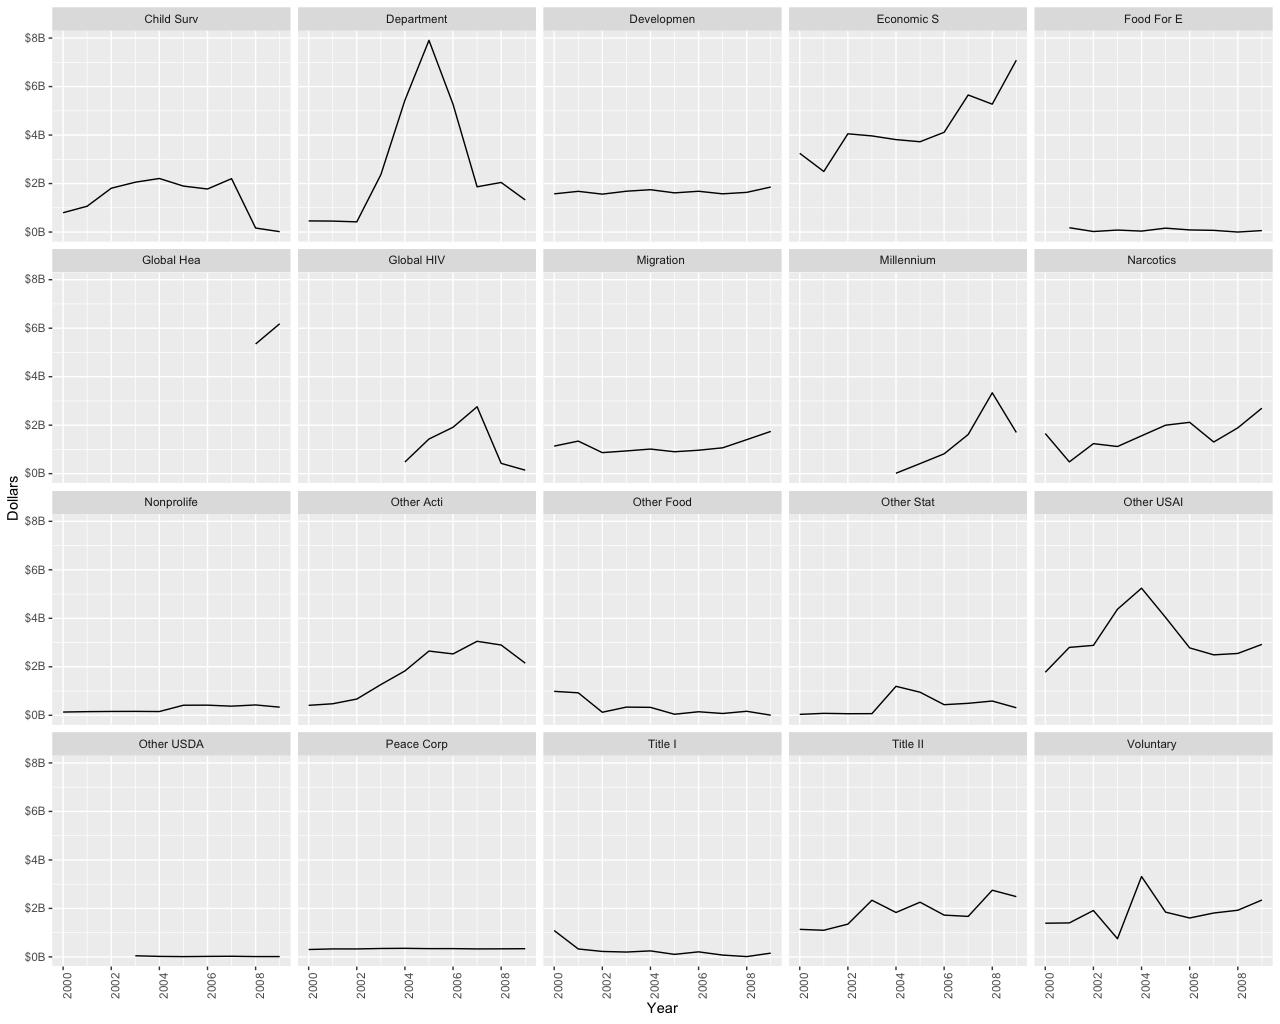
\includegraphics[width=1.0\linewidth]{pic0029}
  \caption{Разход на пари по програми и години}
\label{figure0029}
\end{figure}
\FloatBarrier

Така организирани данните са по редове, за да бъдат трансформирани от редове в колони се използва функцията dcast (Листинг \ref{listing0139}). 

\begin{lstlisting}[caption=От редове към колони, label=listing0139]
melt00 <- melt(Aid_00s, id.vars=c("Country.Name", "Program.Name"), variable.name="Year", value.name="Dollars")
 
cast00 <- dcast(melt00, Country.Name + Program.Name ~ Year, value.var="Dollars")
\end{lstlisting}

Първият аргумент на функцията dcast са данните, които да бъдат използвани. Вторият аргумент е формула на която лявата страна са колоните, които трябва да останат колони. От дясната страна са имената, които трябва да станат колони. Третият аргумент е колоната, която трябва да се използва за попълване на данните в новопоявилите се колони. 

\section{Сложни сливания на данни и трансформация на форматите}

Към вече описаните функции за реорганизация на данните се добавят и функциите от пакетите dplyr и tidyr, които позволяват използването на поточни операции. В някои случаи тези функции имат по-добро бързодействие от предходните. 

\subsection{Привързване на редове и колони}

В пакета dplyr привързването на редове и колони се осъществява с функциите bind\_rows и bind\_cols (Листинг \ref{listing0140}). Тези функции са проектирани да работят с data.frame и tibble обекти. Не могат да работят с вектори и матрици. 

\begin{lstlisting}[caption=Обединяване по колони и редове, label=listing0140]
library(dplyr)
library(tibble)

ds1 <- bind_cols(tibble(TV=c("BNT","bTV","Nova"),Channel=c("1","2","3")), tibble(Rating=c("0.1","0.3","0.2")))

ds2 <- tribble(~TV, ~Channel, ~Rating, "HBO", "4", "0.4", "VH1", "5","0.5", "MTV","6", "0.6")

bind_rows(ds1, ds2)
\end{lstlisting}

И двете функции могат да работят с множество от обекти, едновременно.

\subsection{Сложни сливания на данни}

Пакетът dplyr предлага група от функции за извършване на сливания (joins)\index{сложни сливания}. В множеството данни за диамантите цветът се отбелязва само с една латинска буква, без да има допълнителна информация за значението на самата маркировка. Допълнителна информация за цветовете на диамантите е налична в друго множество от данни, което е много подходящо за демонстрация на сливания между множества данни (Листинг \ref{listing0141}).

\begin{lstlisting}[caption=Сложни сливания, label=listing0141]
library(ggplot2)
library(readr)
library(dplyr)

colors <- as_tibble(read.table("https://raw.githubusercontent.com/TodorBalabanov/Statistical-Data-Processing-with-R/master/data/colors.csv", header=TRUE, sep=","))

left_join(diamonds, colors, by=c('color'='Color')) %>% select(carat, color, price, Description, Details)

tail(right_join(diamonds, colors, by=c('color'='Color')))

inner_join(diamonds, colors, by=c('color'='Color'))

semi_join(colors, diamonds, by=c('Color'='color'))

anti_join(colors, diamonds, by=c('Color'='color'))
\end{lstlisting}

При лявото сливане (left join)\index{сливане от ляво} данните за диамантите са отляво, а данните за цвета са от дясно. Тъй като колоната използвана за ключ се различава в главно и малко C, то ключът се задава с аргумента by. Данните се подават като вектор, където имената на елементите са колоните в лявата таблица, а стойностите са колоните от дясната таблица. При разминаване на типовете за колоните използвани като ключови (фактори със символни низове), то автоматично се прави преобразуване. При лявото сливане участват всички редове от лявата таблица и само редовете, които отговарят по ключ от дясната таблица. 

При десните сливания (right join)\index{сливане от дясно} участват всички редове от дясната таблица, дори и когато няма съответствие по ключа в лявата таблица. При използвания пример, това води до поява на редове съдържащи липсващи стойности (NA), там където няма съответствие.

При вътрешното сливане (inner join)\index{вътрешно сливане} участват само редове, които имат съответствие по ключа и в двете таблици. 

При външното сливане (outer join)\index{външно сливане} участват всички редове и от двете таблици, без значение дали имат съответствие по ключа.

В SQL базите данни няма директен еквивалент, но в R има полусливане (semi join)\index{полусливане}, смисълът на което е, че се всеки ред от лявата таблица се връща първото срещане в дясната таблица. По-своята същност това е филтриране по редове. Връщат се само редове, които отговарят на съответствие по ключ. 

Противоположното действие на полусливането в R се постига с anti join\index{анти сливане}. Смисълът е, че се връщат тези редове от лявата таблица, които нямат съответствие по ключ в дясната таблица. 

\subsection{Реформатиране на данните}

Размяната на колони с редове и обратното бе демонстрирана с функциите melt и dcast. Подобна реорганизация по редове и колони може да се постигне с функциите gather и spread от пакета tidyr. 

\begin{lstlisting}[caption=Данни за реакциите, label=listing0142]
library(readr)

emotions <- read_tsv("https://raw.githubusercontent.com/TodorBalabanov/Statistical-Data-Processing-with-R/master/data/reaction.txt")
Parsed with column specification:
cols(
  ID = col_integer(),
  Test = col_integer(),
  Age = col_double(),
  Gender = col_character(),
  BMI = col_double(),
  React = col_double(),
  Regulate = col_double()
\end{lstlisting}

За демонстрация на трансформацията от колони към редове е използвано множеството данни от Columbia University, което изследва емоционалните реакции и задръжки (Листинг \ref{listing0142}). Тъй като данните са в обикновен текстов файл и като разделител се използва символа за табулация, за тяхното прочитане се използва функцията read\_tsv (Tab Separated Values). Данните се зареждат в tibble обект, като за всяка колона се избира подходящ тип данни. 

\begin{lstlisting}[caption=Свиване от колони в редове, label=listing0143]
library(tidyr)

emotions %>% gather(key=Type, value=Measurement, Age, BMI, React, Regulate)

gather(emotions, key=Type, value=Measurement, -ID, -Test, -Gender)
\end{lstlisting}

Данните за емоциите са организирани на колони (wide format)\index{широк запис}. С функцията gather част от колоните са трансформирани в редове (long format)\index{дълъг запис}. При събирането на данните, за всяко наблюдавано лице, измерванията са записани в следните четири колони Age, BMI, React и Regulate. Така оформени данните са неподходящи за някои видове пресмятания и поради тази причина е разумно четирите вида измервания да бъдат в една колона (Measurement), а втора колона (Type) да показва за кой тип измерване е стойността (Листинг \ref{listing0143}). С функцията gather се получава своеобразно събиране на стойностите от няколко колони в една. Първият аргумент е множеството данни, вторият аргумент ключът за новосъздадената колона, следва колоната със стойностите и след това се изброяват колоните, които формират общата колона със стойности. В оригиналните данни идентификаторът на изследвания обект присъства на два реда (два проведени експеримента), а в трансформираните данни идентификаторът на изследвания обект присъства на осем реда, тъй като за всеки експеримент са добавени по четири реда за различните видове измервания. Възможно е да се направи същата трансформация с изрично изброяване на колоните, които не трябва да бъдат събирани. Тогава се използва символът тилда пред имената на колоните. 

\begin{lstlisting}[caption=Разпъване от редове в колони, label=listing0144]
library(dplyr)

emotions %>% gather(key=Type, value=Measurement, Age, BMI, React, Regulate) %>% arrange(ID)

emotions %>% spread(key=Type, value=Measurement)
\end{lstlisting}

Обратното действие на събирането е разпъване в колони и в пакета tidyr то се постига с функцията spread (Листинг \ref{listing0144}). Аргументът key определя имената на колоните които ще бъдат създадени. Аргументът value определя кои стойности ще бъдат използвани за попълване на новосъздадените колони. 

\section{Работа със символни низове}

Работата със символни низове\index{символни низове} е много често срещана при обработката на статистически данни. Не рядко информацията е представена в чист текст (plain text). В R символни низове могат да се конструират или да бъдат изследвани, примерно с регулярни изрази. Пакетът stringr дава набор от функции за работа със символни низове.

\subsection{Формиране на текст}

Слепването (конкатенация)\index{конкатенация на символни низове} на символни е една от най-често срещаните операции и в R тя може да се постигне с функцията paste (Листинг \ref{listing0145}). Ако не бъде зададен разделител, по подразбиране се използва символът интервал. Функцията paste е векторизирана и към нея могат да се подават аргументи под формата на вектори от символни низове. Важното е векторите да са с еднакви размери, така че елементите им да бъдат групирани по индекс. Функцията може да се използва и за слепване на вектор от символни низове, чрез разделител зададен в параметъра collapse. 

\begin{lstlisting}[caption=Конкатенация на символни низове, label=listing0145]
paste("Hello", "world", "!")

paste(c("Hello", "world", "!"), collapse=" ")
\end{lstlisting}

Функцията paset е полезна за формирането на по-кратки текстове, но когато се работи със сложен или дълъг текст, в който трябва да се появят стойности на различни променливи, то функцията sprintf дава много повече възможности (Листинг \ref{listing0146}). 

\begin{lstlisting}[caption=Разпъване от редове в колони, label=listing0146]
name = "Todor"
sprintf("Hello, %s!", name)
\end{lstlisting}

Функцията sprintf дава изключително много възможности за форматирането на текст и е позната още от библиотеките на програмния език C. Както много други функции в R, sprintf e векторизирана. 

\subsection{Извличане на текст}

В практиката информацията често се получава в неструктуриран вид (предимно текстов формат) и в такива случаи се налага извличане на нужните данни, чрез анализ на неструктурирания поток (Листинг \ref{listing0147}). 

\begin{lstlisting}[caption=Извличане на текст, label=listing0147]
library(XML)

presidents <- readHTMLTable("http://www.loc.gov/rr/print/list/057_chron.html", which=3, as.data.frame=TRUE, skip.rows=1, header=TRUE, stringsAsFactors=FALSE)

library(stringr)

years <- str_split(string=presidents$YEAR, pattern="-")

ranges <- data.frame(Reduce(rbind, years))
names(ranges) <- c("Start", "Stop")

presidents <- cbind(presidents, ranges)
presidents$Start <- as.numeric(as.character(presidents$Start))
presidents$Stop <- as.numeric(as.character(presidents$Stop))

presidents[str_sub(string=presidents$Start, start=4, end=4) == 1, c("YEAR", "PRESIDENT", "Start", "Stop")]
\end{lstlisting}

При четенето на неструктуриранеи данни често в данните има нежелана информация и се налага допълнително коригиране. Първо трябва да се разделят годините, които са отделни с тире (-). Следва добавяне на две колони за начало и край. С помощта на функцията str\_sub може да се използва част от символен низ. 

\begin{lstlisting}[caption=Регуларни изрази, label=listing0148]
presidents[str_detect(string=presidents$PRESIDENT, pattern="John"), c("YEAR", "PRESIDENT", "Start", "Stop")]

sum( str_detect(presidents$PRESIDENT, "john") )
sum( str_detect(presidents$PRESIDENT, ignore.case("John")) )
\end{lstlisting}

При търсенето на по-сложен шаблон в текст едно от най-мощните средства са регулярните изрази\index{регулярни изрази} (Листинг \ref{listing0148}). Регулярните изрази са реализация на краен автомат по дефиниран шаблон. Езикът на регулярните изрази е твърде сложен за да бъде детайлно представен в настоящото изложение, поради тази причина се представят само няколко илюстративни примери. 

\begin{lstlisting}[caption=Сложни регуларни изрази, label=listing0149]
conncetion <- "https://github.com/TodorBalabanov/Statistical-Data-Processing-with-R/raw/master/data/war.rdata"

load(conncetion)
close(connection)

wars[str_detect(string=wars, pattern="-")]
str_split(string=wars, pattern="(ACAEA)|-", n=2)
\end{lstlisting}

Зареждането на бинарни файлове е малко по-различно от CSV файлове и това налага използване на функцията load (Листинг \ref{listing0149}). Определянето на началото на всяка война става с функцията str\_detect. Разделянето на символен низ, по зададен сепаратор, се извършва с функцията str\_split.  Функцията str\_trim служи за премахване на „белите“ полета пред или след символния низ. За премахване на конкретна дума се използва функцията str\_extract. Заместването по шаблон при първо срещане става с функцията str\_replace, а на всяко срещане str\_replace\_all. 

\section*{Заключение}

Реорганизирането на данните в подходяща форма е от ключово значение в процеса по осъществяването на статистически анализ. Този процес често включва преработката на колони в редове и обратното или сливане на различни множества от данни. Често в практиката данните са представени в текстов вид и това налага определени трансформации, така че данните да бъдат използваеми в съответните статистически пресмятания. 


\newpage
\chapter{Разширени графични възможности и вероятностни разпределения}
\label{chapter08}

\section{Разширени графични възможности}

Към базовите графични възможности на R, пакетите ggplot2 и lattice добавят множество допълнителни функционалности. Синтаксисът на извикванията леко се различава от този на функциите в базовите възможности, но това създава затруднения само в началния етап от употребата на двата пакета. 

За визуализация, чрез ggplot2 като основа се използва функцията ggplot. В общия случай тази функция получава, като входен параметър данните за визуализиране и понякога някои допълнителни параметри. Резултатът от изпълнението на ggplot е обект, който в последствие може да бъде допълнително променян, чрез добавяне на възможности с помощта на операцията събиране (+). 

\subsection{Хистограми и плътности}

Хистограмата служи за групиране на стойностите и изброяване на това колко стойности попадат по определените групи. Размерът на всяка група (bin) определя ширината на стълба. 

\begin{lstlisting}[caption=Хистограма и плътност, label=listing0150]
library(ggplot2)

ggplot(data=diamonds) + geom_histogram(aes(x=carat))

ggplot(data=diamonds) + geom_density(aes(x=carat),fill="grey50")
\end{lstlisting}

Както и в предходния пример за хистограма, тук също е представено разпределението на диамантите по карати (Листинг \ref{listing0150}).

\begin{figure}[h!]
  \centering
  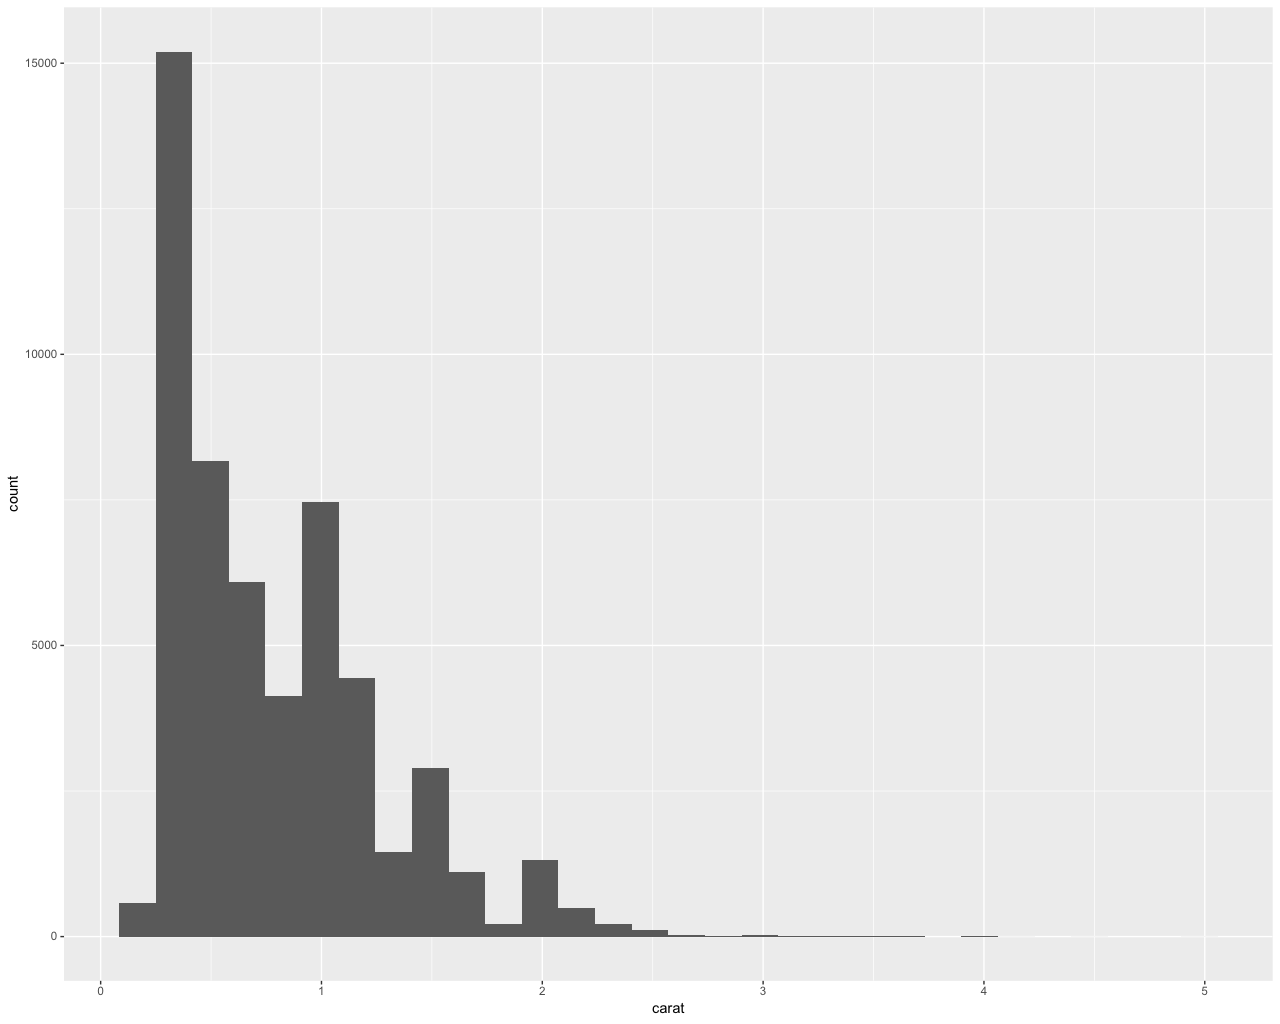
\includegraphics[width=1.0\linewidth]{pic0030}
  \caption{Хистограма при 30 групи}
\label{figure0030}
\end{figure}
\FloatBarrier

Функцията aes определя кои данни да бъдат използвани за разполагане по осите. В примера с диамантите, това е характеристиката за тегло (карат). 

\begin{figure}[h!]
  \centering
  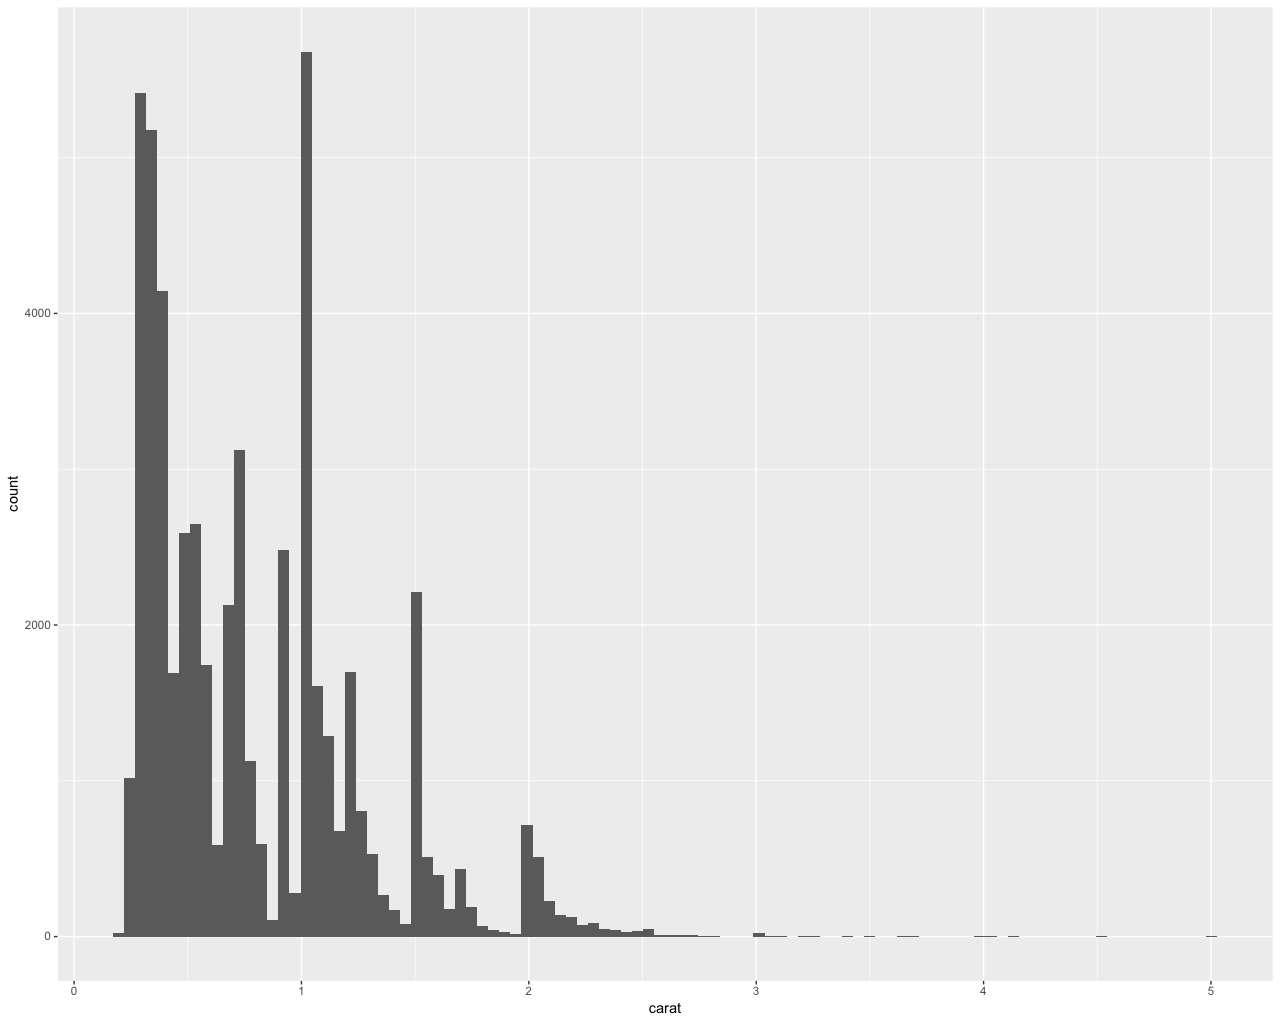
\includegraphics[width=1.0\linewidth]{pic0031}
  \caption{Хистограма при 100 групи}
\label{figure0031}
\end{figure}
\FloatBarrier

Размерът на групите в хистограмата може да варира (Фиг. \ref{figure0030},\ref{figure0031}). За да се изчертае плътностна функция е достатъчно графичният обект, генериран от ggplot, да бъде декориран с функцията geom\_density (Фиг. \ref{figure0032}), вместо с функцията geom\_histogram. 


\begin{figure}[h!]
  \centering
  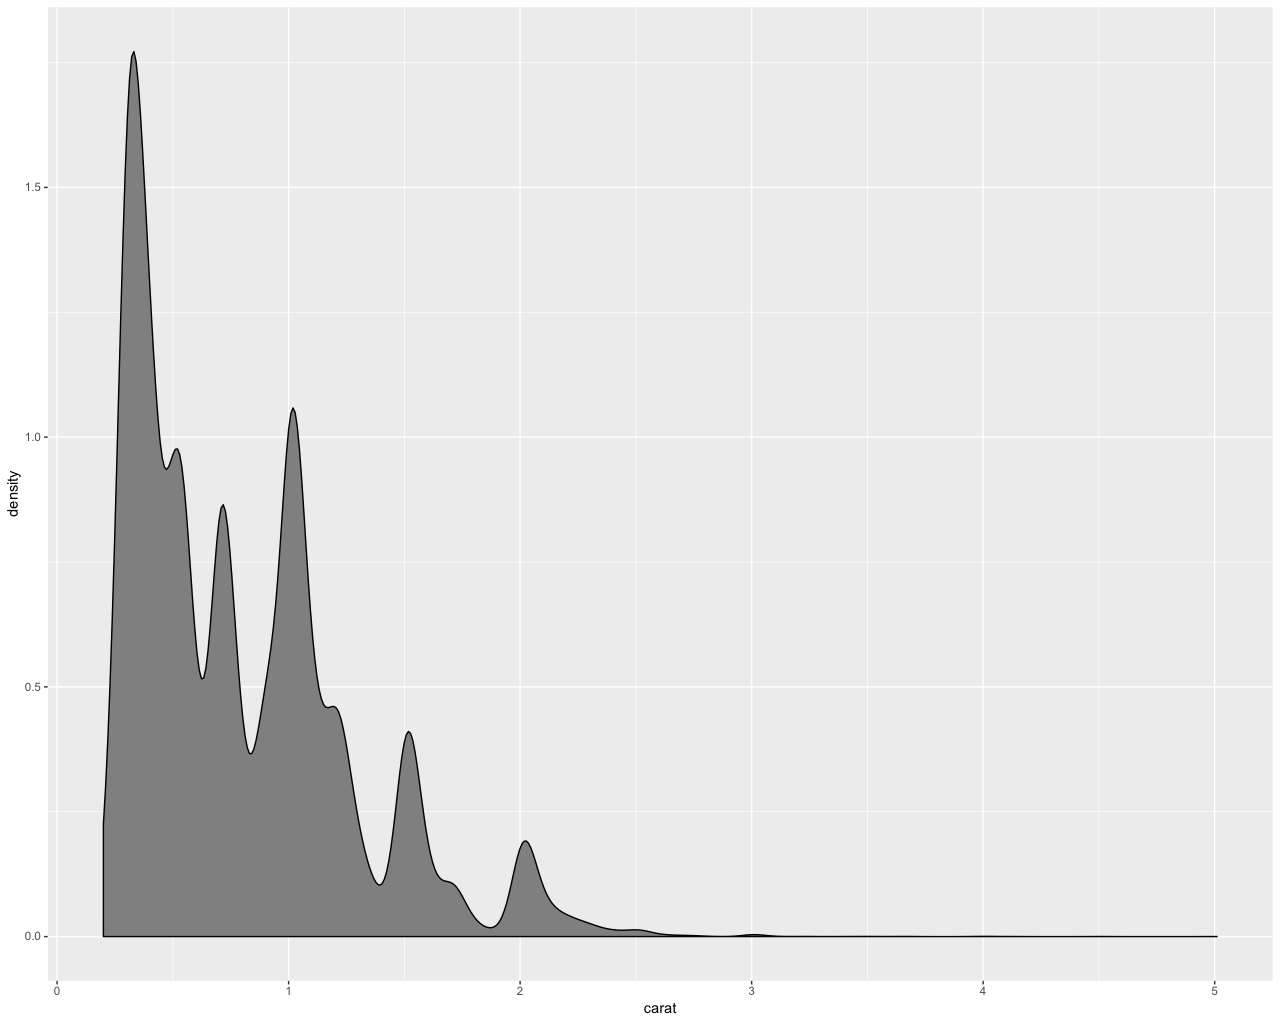
\includegraphics[width=1.0\linewidth]{pic0032}
  \caption{Плътностна функция}
\label{figure0032}
\end{figure}
\FloatBarrier

Хистограмата показва броене по групи, докато плътностната функция задава вероятността определен камък да попадне в предварително определен интервал. Макар и много да си приличат, хистограмата и плътностната функция са подходящи в два различни случая. Хистограмите са полезни при дискретни случайни величини, докато плътностните функции намират повече употреба в непрекъснатите случайни величини. 

\subsection{Диаграми на разсейване}

Пакетът ggplot2 разширява възможностите за визуализация на диаграми на разпръскване, които базовата функционалност на R предлага (Листинг \ref{listing0151}). 

\begin{lstlisting}[caption=Диаграма на разпръскване с ggplot2, label=listing0151]
library(ggplot2)
ggplot(diamonds, aes(x=carat, y=price)) + geom_point()
\end{lstlisting}

Функцията aes определя кои колони от множеството данни да се използват при визуализацията (Фиг. \ref{figure0033}). Пакетът ggplot2 дава и друго много съществено предимство, графиката която ще се изчертава да бъде съхранена в отделен обект, на който обект след това да се добавят различни визуални декорации (обектът c2p от примера).

\begin{figure}[h!]
  \centering
  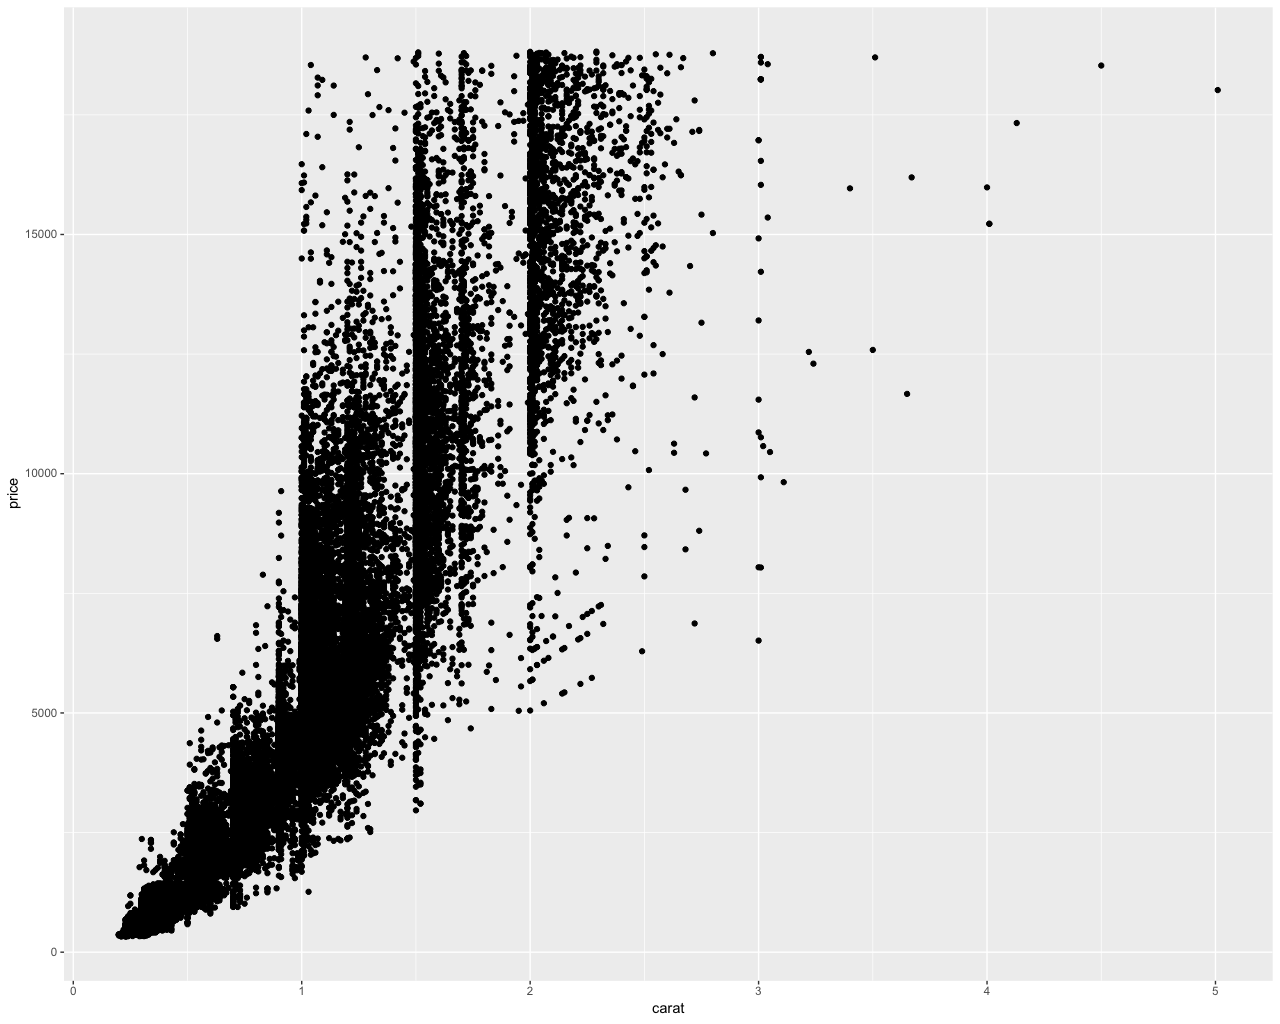
\includegraphics[width=1.0\linewidth]{pic0033}
  \caption{Диаграма на разпръскване с ggplot2}
\label{figure0033}
\end{figure}
\FloatBarrier

Пакетът дава възможности и за подреждането на група от диаграми на разсейването. Това се постига с някоя от функциите facet\_wrap или facetю\_grid (Листинг \ref{listing0152}). 

\begin{lstlisting}[caption=Диаграма на разпръскване групирани по признак, label=listing0152]
c2p <- ggplot(diamonds, aes(x=carat, y=price))

c2p + geom_point(aes(color=color)) + facet_wrap(~color)

c2p + geom_point(aes(color=color)) + facet_grid(clarity~cut)
\end{lstlisting}

Функцията facet\_wrap разделя множеството от данните на групи, според зададения признак (в примера това е цветът на диамантите) и след това формира диаграма на разпръскване за всяка от групите (Фиг. \ref{figure0034}).

\begin{figure}[h!]
  \centering
  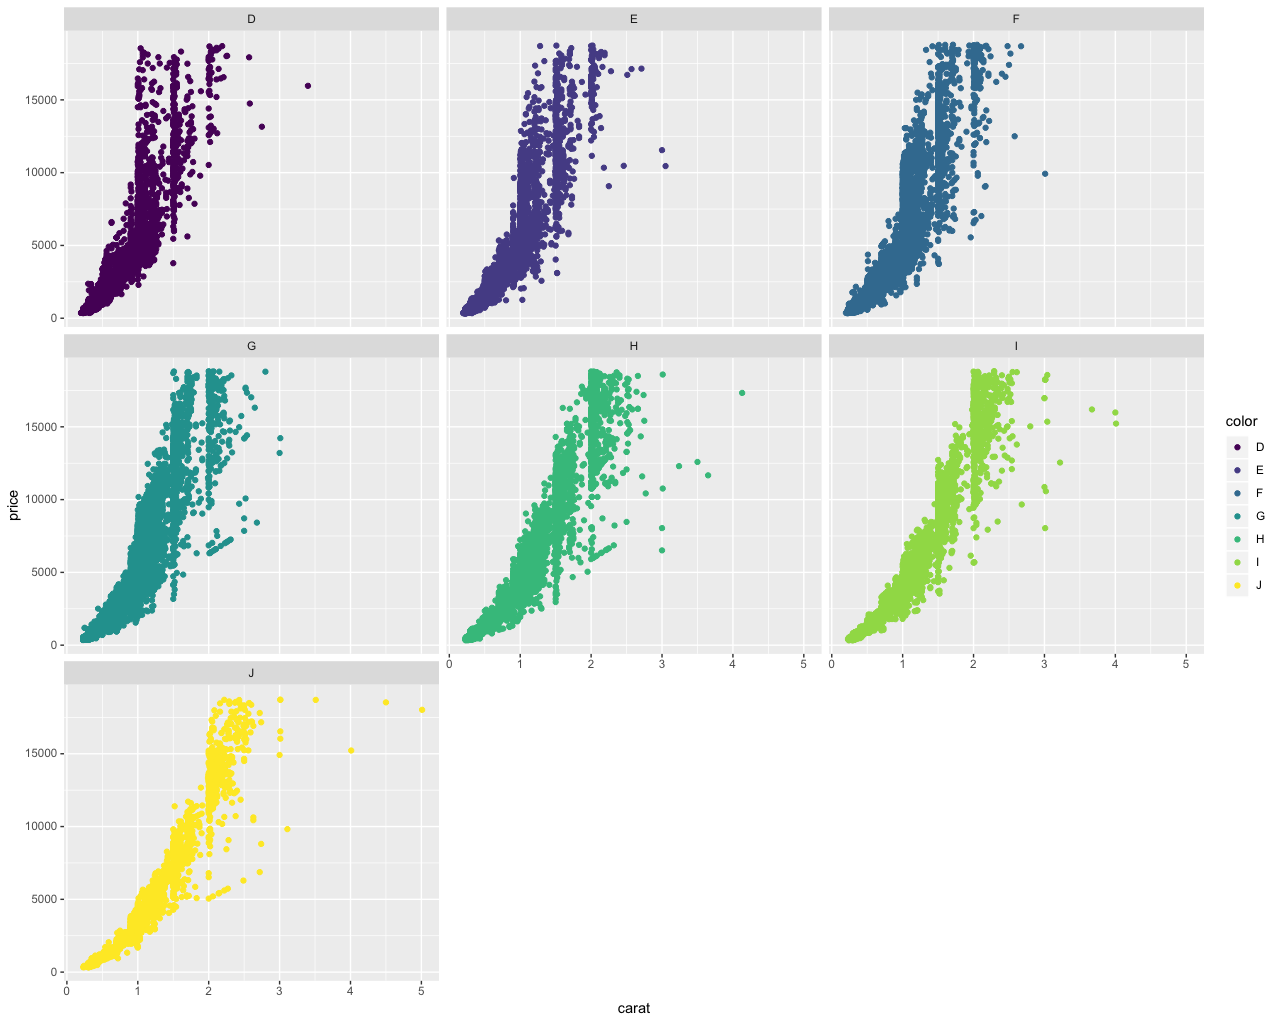
\includegraphics[width=1.0\linewidth]{pic0034}
  \caption{Диаграма на разпръскване по групи за цвят на диамантите}
\label{figure0034}
\end{figure}
\FloatBarrier

Функцията facet\_grid действа по сходен начин, но всички стойности на признака за групиране се отразяват на осите за всяка от графиките (Фиг. \ref{figure0035}). Важно е да се забележи начина по който са ориентирани осите на всяка от подграфиките. Ориентацията пряко зависи дали признакът за чистота е от ляво, а признакът за качество на среда от дясно или обратното. 

\begin{figure}[h!]
  \centering
  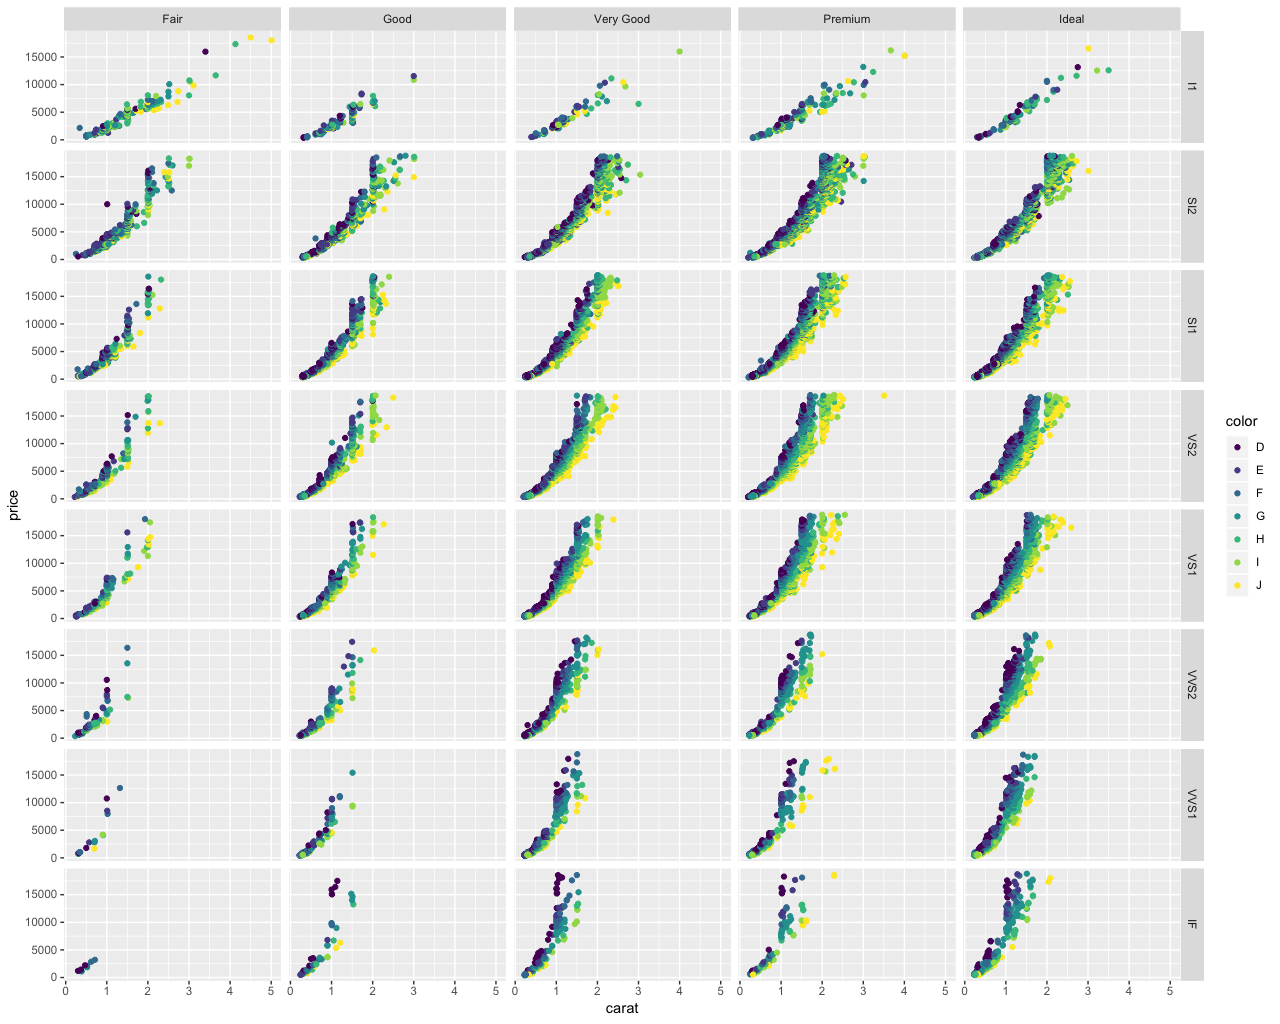
\includegraphics[width=1.0\linewidth]{pic0035}
  \caption{Визуализация с групиране по два признака}
\label{figure0035}
\end{figure}
\FloatBarrier

Организацията на графики по групи е възможна с различни графични представяния, като пример е представянето на хистограма в групи по качество на сряза (Фиг. \ref{figure0036}).

\begin{figure}[h!]
  \centering
  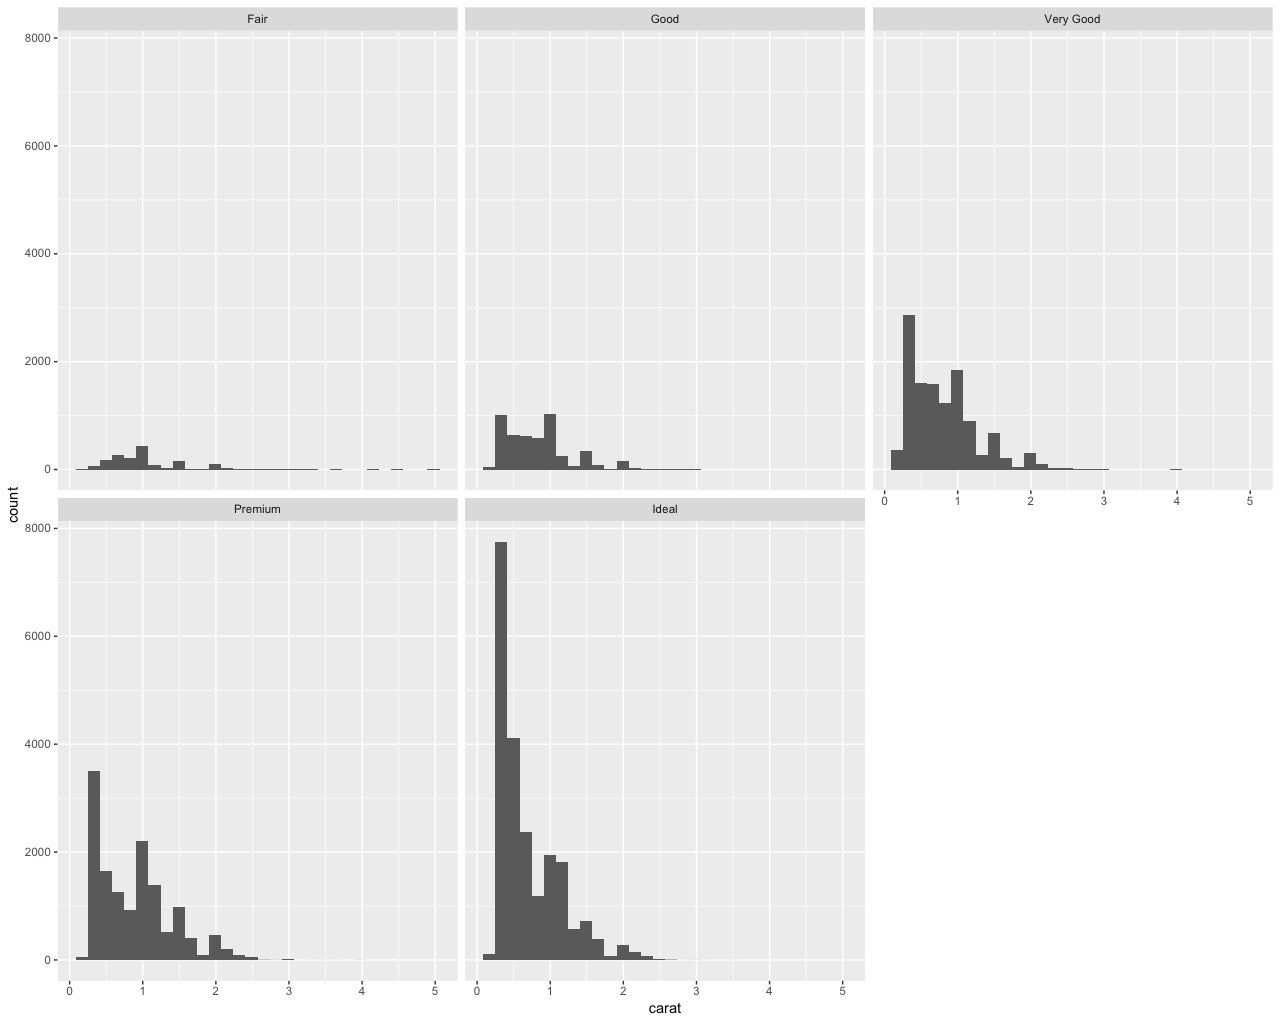
\includegraphics[width=1.0\linewidth]{pic0036}
  \caption{Визуализация на хистограми с групиране}
\label{figure0036}
\end{figure}
\FloatBarrier

\subsection{Графики тип кутия и цигулка}

Пакетът ggplot2 дава възможност за визуализация на графики тип кутия (Листинг \ref{listing0153}).

\begin{lstlisting}[caption=Визуализация тип кутия, label=listing0153]
ggplot(diamonds, aes(y=depth)) + geom_boxplot()

ggplot(diamonds, aes(y=depth, x=cut)) + geom_boxplot()

ggplot(diamonds, aes(y=depth, x=cut)) + geom_boxplot() + geom_violin()

ggplot(diamonds, aes(y=depth, x=cut))+ geom_point() + geom_violin()
\end{lstlisting}

При обща визуализация на данните, без да се търси групиране по признан за абсцисната ос може да не се подава стойност (Фиг. \ref{figure0037}). 

\begin{figure}[h!]
  \centering
  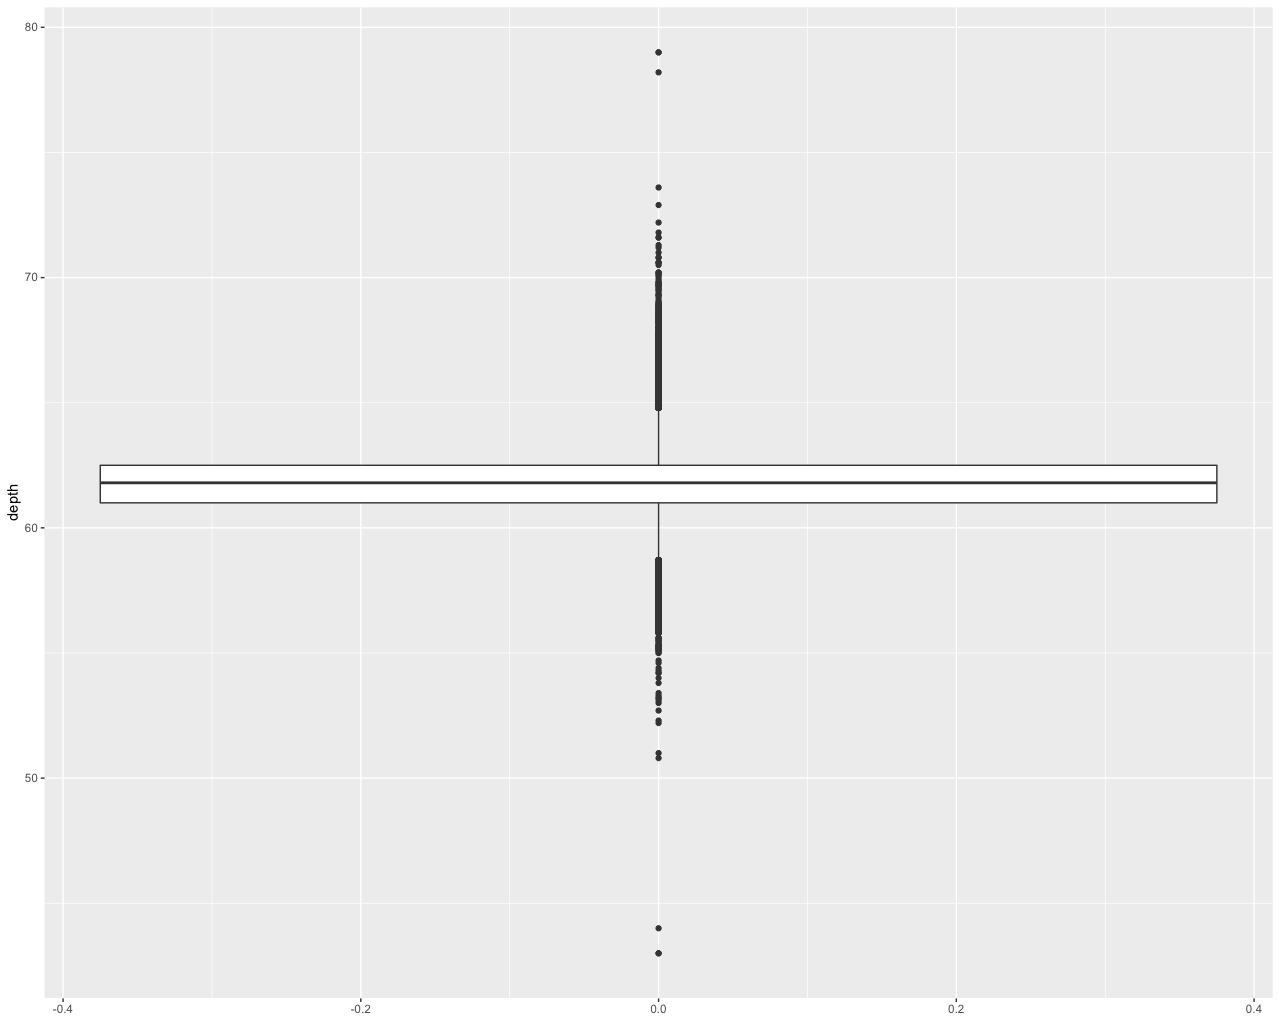
\includegraphics[width=1.0\linewidth]{pic0037}
  \caption{Визуализация на характеристиката за дълбочина на диамантите}
\label{figure0037}
\end{figure}
\FloatBarrier

Визуализацията на графики от тип кутия, с групиране по признак се реализира чрез подаване на колоната, по която да се групира, като параметър за абцисна ос, на функцията aes (Фиг. \ref{figure0038}).

\begin{figure}[h!]
  \centering
  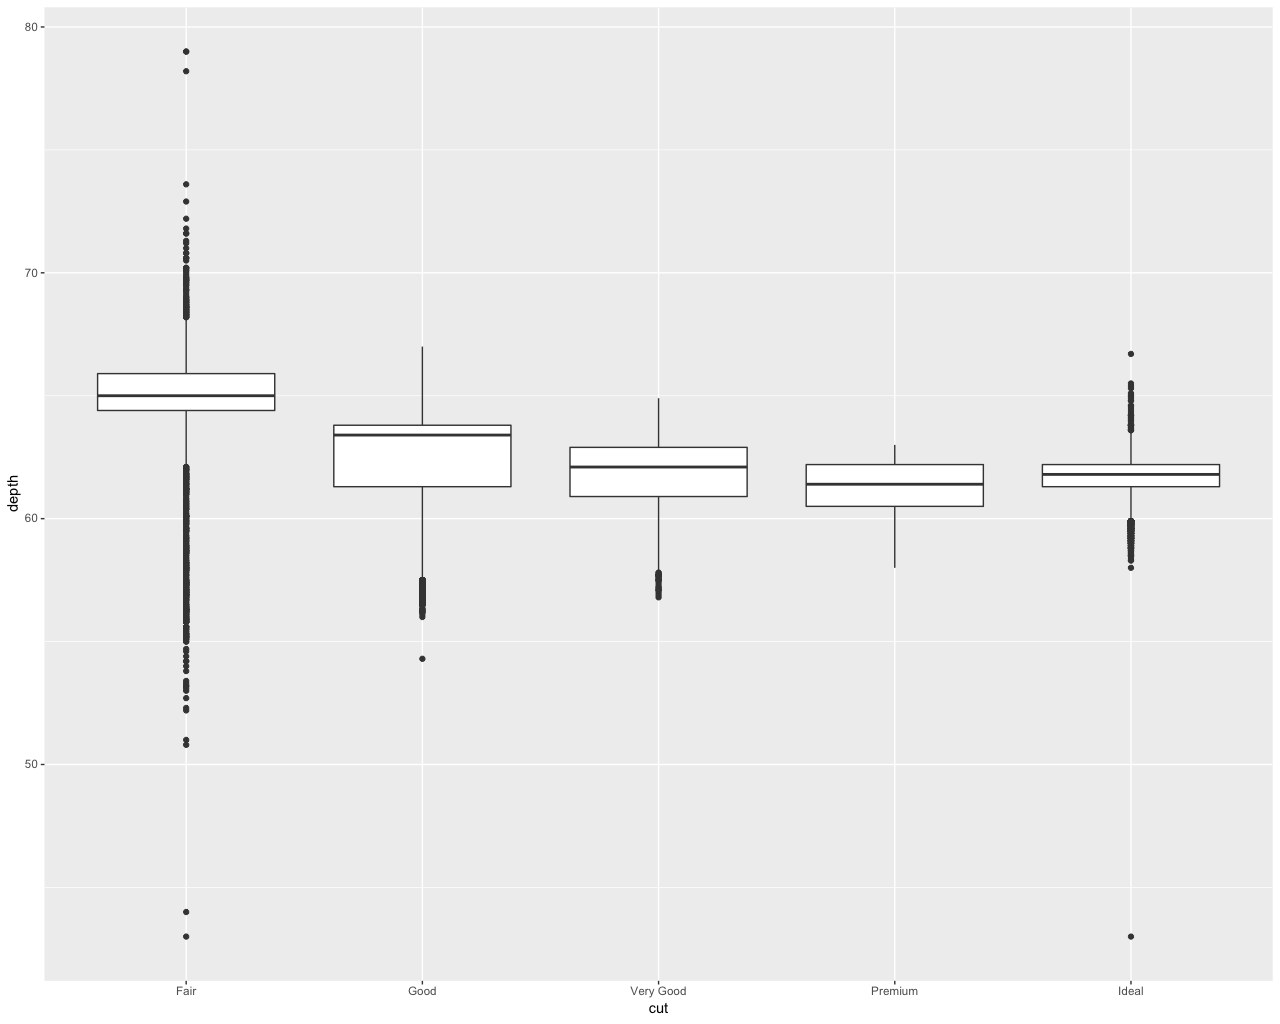
\includegraphics[width=1.0\linewidth]{pic0038}
  \caption{Dълбочина на диамантите в групи според сряза}
\label{figure0038}
\end{figure}
\FloatBarrier

От графика тип кутии много лесно се преминава към графика от тип цигулки, чрез подмяна на декориращата функция (Фиг. \ref{figure0039}).

\begin{figure}[h!]
  \centering
  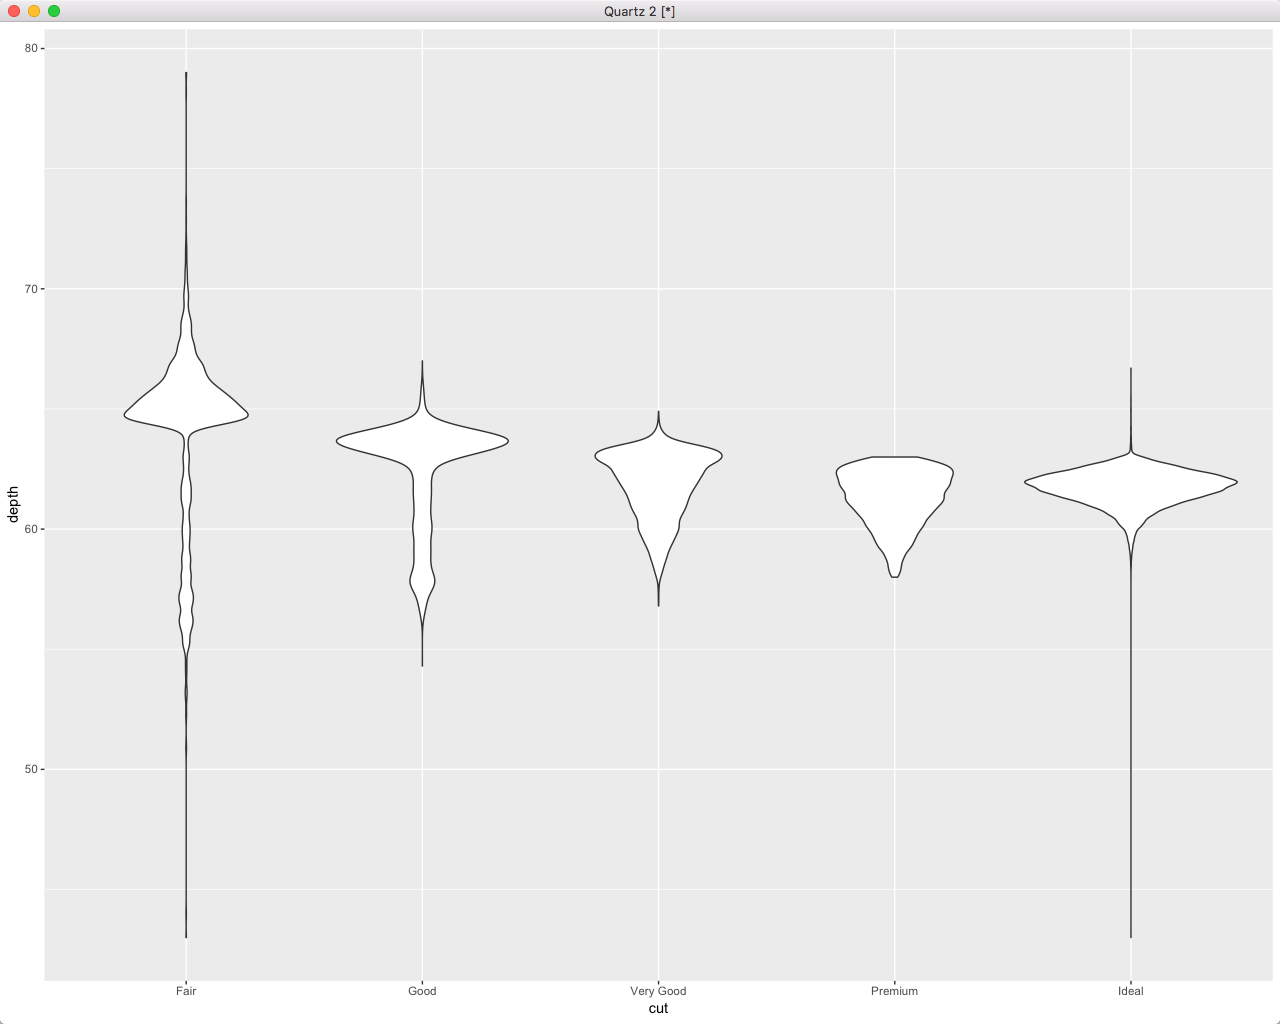
\includegraphics[width=1.0\linewidth]{pic0039}
  \caption{Графика тип цигулки}
\label{figure0039}
\end{figure}
\FloatBarrier

Графиките тип кутия и тип цигулка си приличат, като основната разлика е, че цигулките имат повече смисъла на плътностна функция и носят повече информация, отколкото правите ръбове на кутиите. 

\begin{figure}[h!]
  \centering
  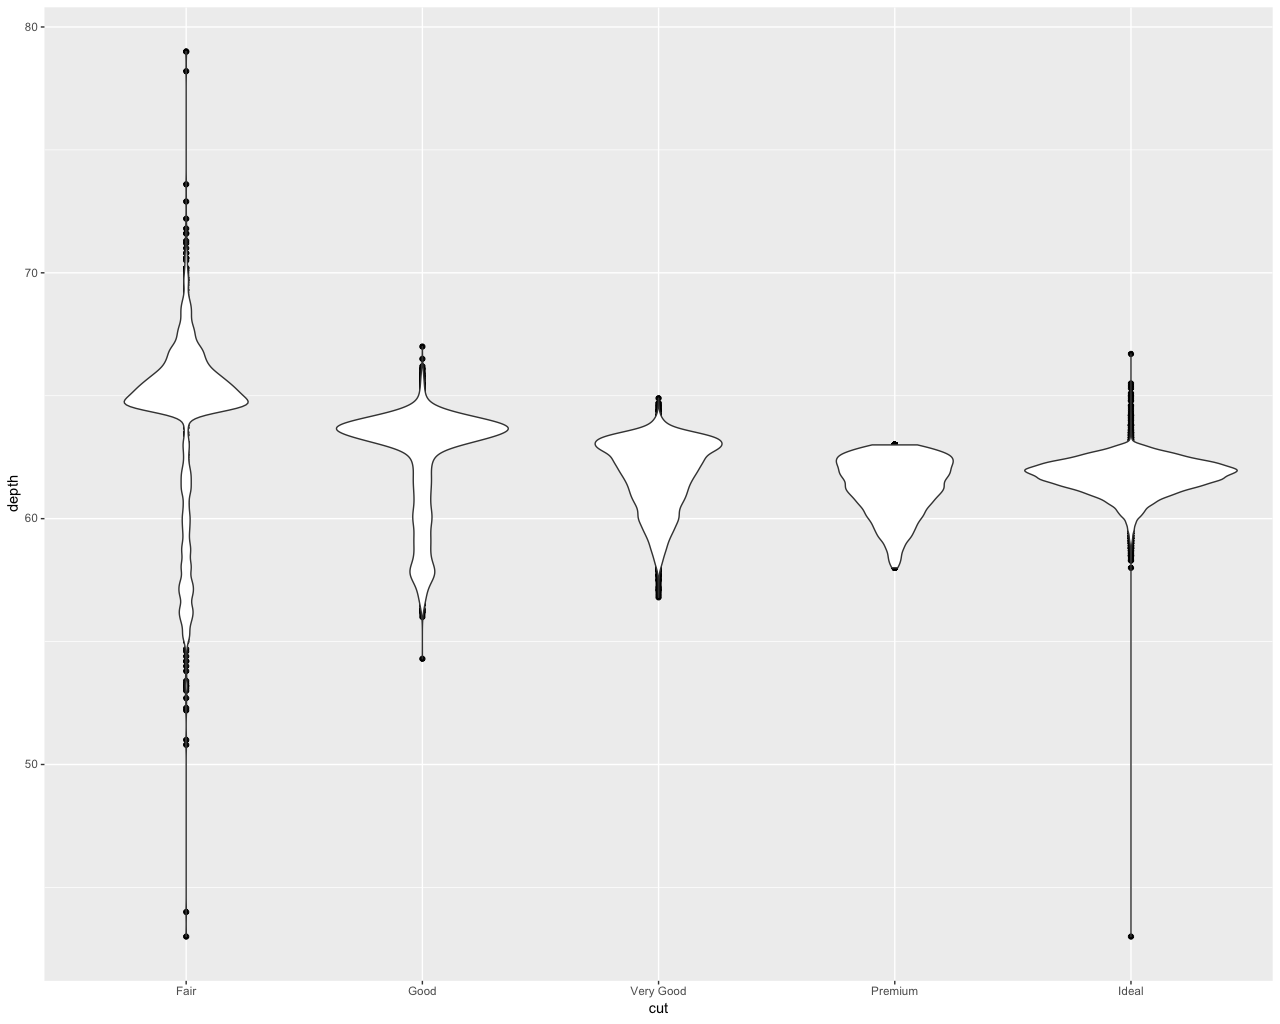
\includegraphics[width=1.0\linewidth]{pic0040}
  \caption{Добавяне на декорация с точки}
\label{figure0040}
\end{figure}
\FloatBarrier

Декорациите за визуализация на данните може да се наслагват една върху друга, като от съществено значение е редът на изчертаването им (Фиг. \ref{figure0040}). Ако декорацията с точките бъде добавена след декорацията с цигулките, точки ще се появят и върху самите цигулки. 

\subsection{Линейни графики}

В определени случаи най-удачно е визуалното представяне на информацията да бъде извършено с линейни графики. Линейната графика е удачна примерно при представянето на тренд (Листинг \ref{listing0154}).

\begin{lstlisting}[caption=Линейни графики, label=listing0154]
library(lubridate)

ggplot(economics, aes(x=date, y=pop)) + geom_line()

economics$year <- year(economics$date)
economics$month <- month(economics$date, label=TRUE)

library(scales)

ggplot(economics, aes(x=month, y=pop)) + geom_line(aes(color=factor(year), group=year)) + scale_color_discrete(name="Year") + scale_y_continuous(labels=comma)+ labs(title="Population Growth", x="Month", y="Population")
\end{lstlisting}

В примерните данни за икономическо развитие, нарастването на популацията във времето е представена под формата на линейна графика (Фиг. \ref{figure0041}).

\begin{figure}[h!]
  \centering
  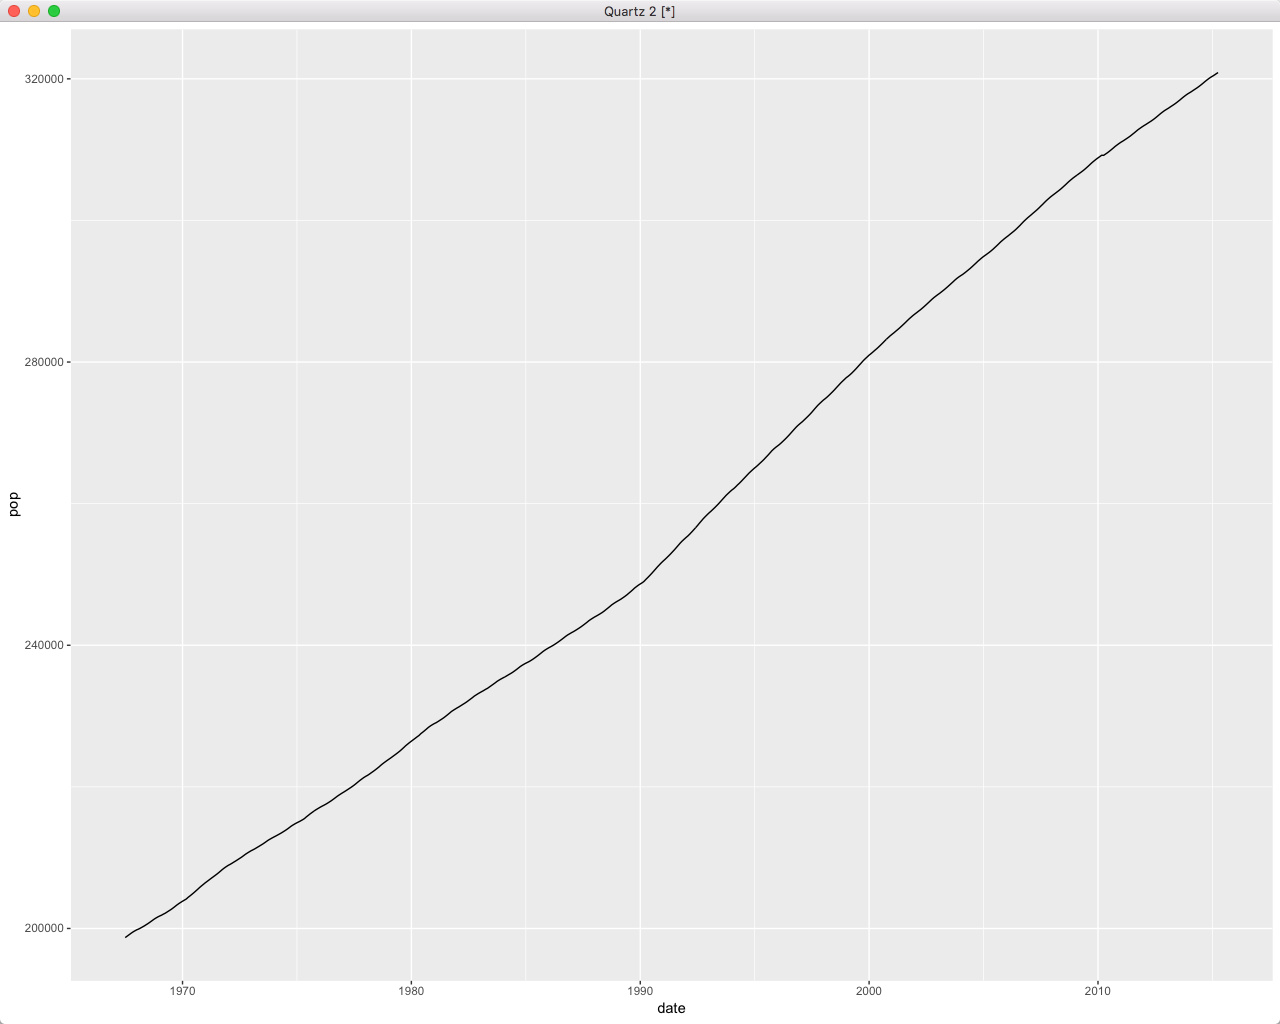
\includegraphics[width=1.0\linewidth]{pic0041}
  \caption{Нарастване на популацията във времето}
\label{figure0041}
\end{figure}
\FloatBarrier

При анализирането на ръст в популацията понякога е интересно тази информация да се организира по години и да се представи в обща графика. Данните за всяка година могат да се представят с различен цвят, така че да бъде ясно кои линии за кои периоди от време се отнасят. С помощта на библиотеката lubridate в economics данните се добавят две допълнителни колони за година и за месец. С помощта на библиотеката scales се постига по-добро оформление на информацията по осите. 

\begin{figure}[h!]
  \centering
  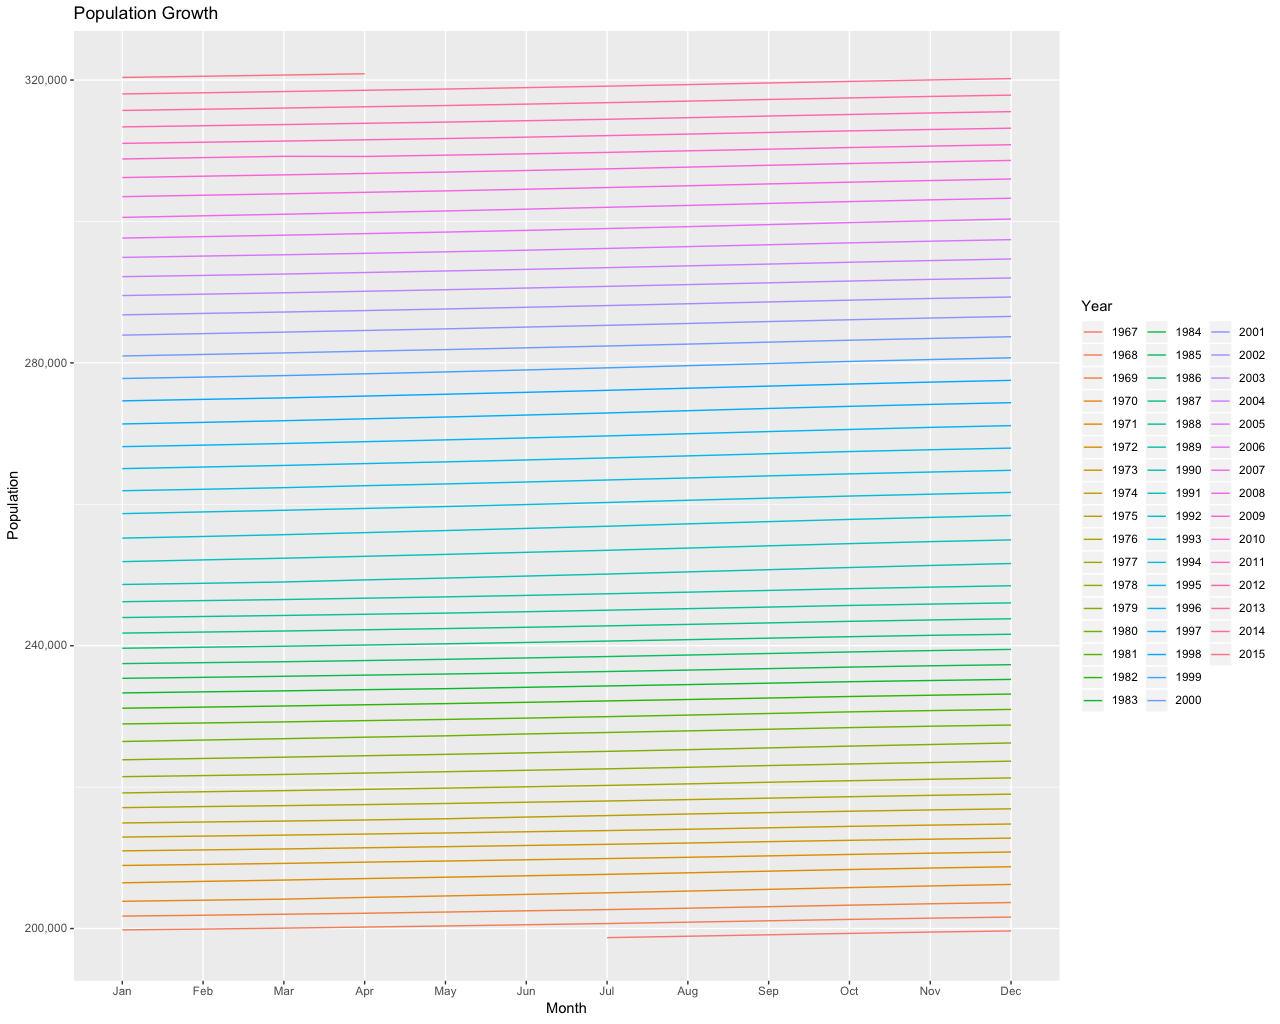
\includegraphics[width=1.0\linewidth]{pic0042}
  \caption{Визуализиране на приръста по години}
\label{figure0042}
\end{figure}
\FloatBarrier

Важно е да се отбележи, че информацията за годината е от тип factor, така че да се използва за определяне на цветовете. Също така на ординатната ос се добавя и запетая, като разделител за хилядите. Като последна декорация е подмяната на текстовете за двете оси. 

\subsection{Тематично оформление}

При генерирането на графики е от съществено значение медията на която тези графики ще бъдат представяни. При визуализация на проектор или монитор може да се използват тематично тъмни цветове, а при разпечатване на хартия е по-разумно да се използват светли цветове, така че да се намалява разхода на мастило (Листинг \ref{listing0155}). Каквито и да са нуждите за представяне, в пакетът ggthemes са добавени възможности за цялостно преобразяване на получените графики, чрез избор на теми (Фиг. \ref{figure0043}-\ref{figure0046}).

\begin{lstlisting}[caption=Избор на теми за визуално представяне, label=listing0155]
library(ggthemes)

ggplot(diamonds, aes(x=carat, y=price)) + geom_point(aes(color=color)) + theme_wsj()

ggplot(diamonds, aes(x=carat, y=price)) + geom_point(aes(color=color)) + theme_tufte()

ggplot(diamonds, aes(x=carat, y=price)) + geom_point(aes(color=color)) + theme_excel()

ggplot(diamonds, aes(x=carat, y=price)) + geom_point(aes(color=color)) +  theme_economist() + scale_colour_economist()
\end{lstlisting}

\begin{figure}[h!]
  \centering
  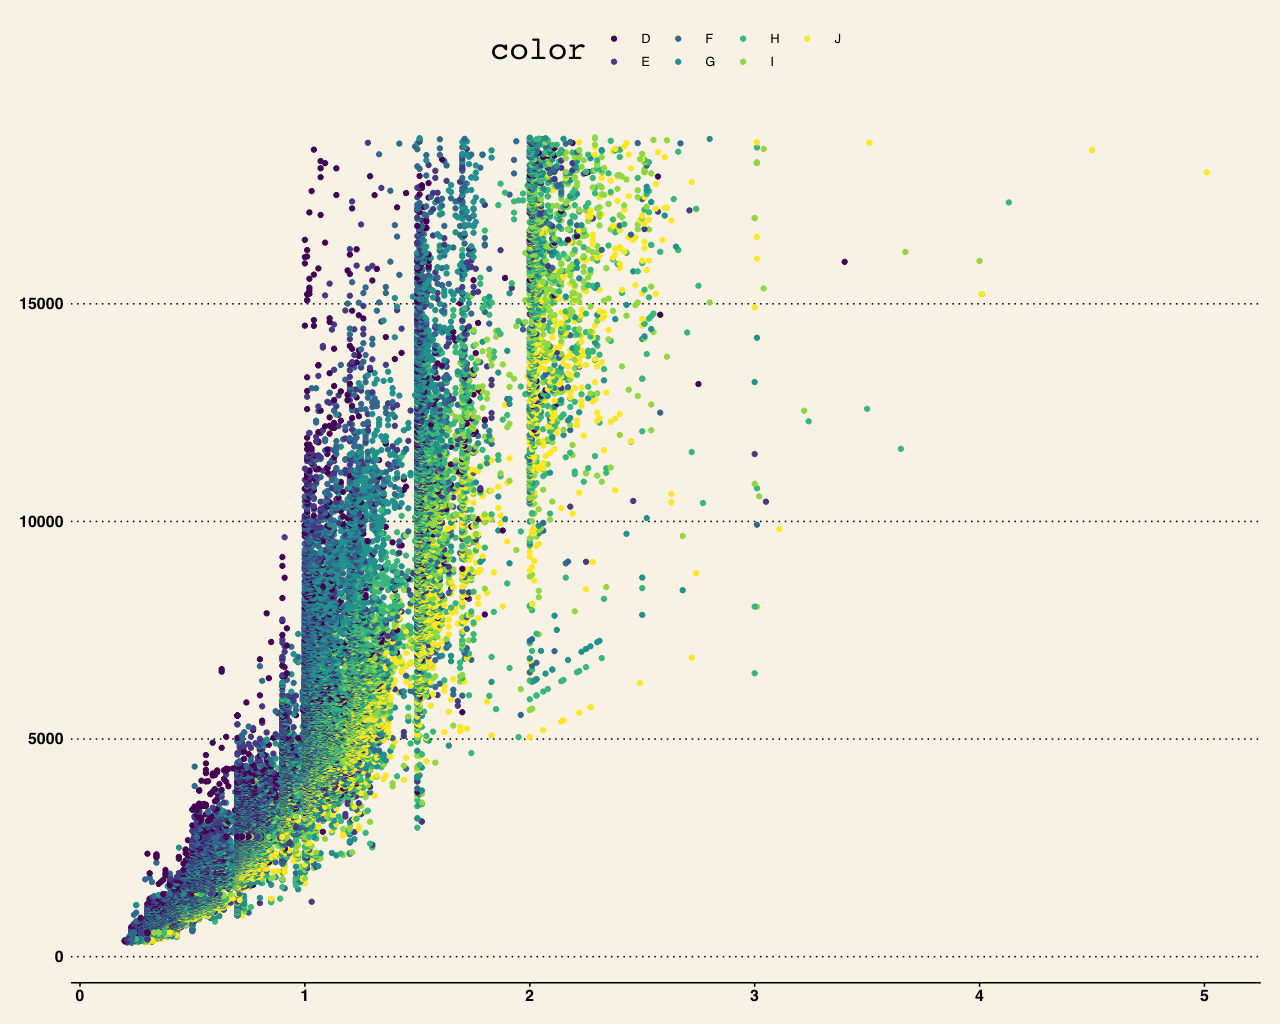
\includegraphics[width=1.0\linewidth]{pic0043}
  \caption{Тема Wall Street Journal}
\label{figure0043}
\end{figure}
\FloatBarrier

\begin{figure}[h!]
  \centering
  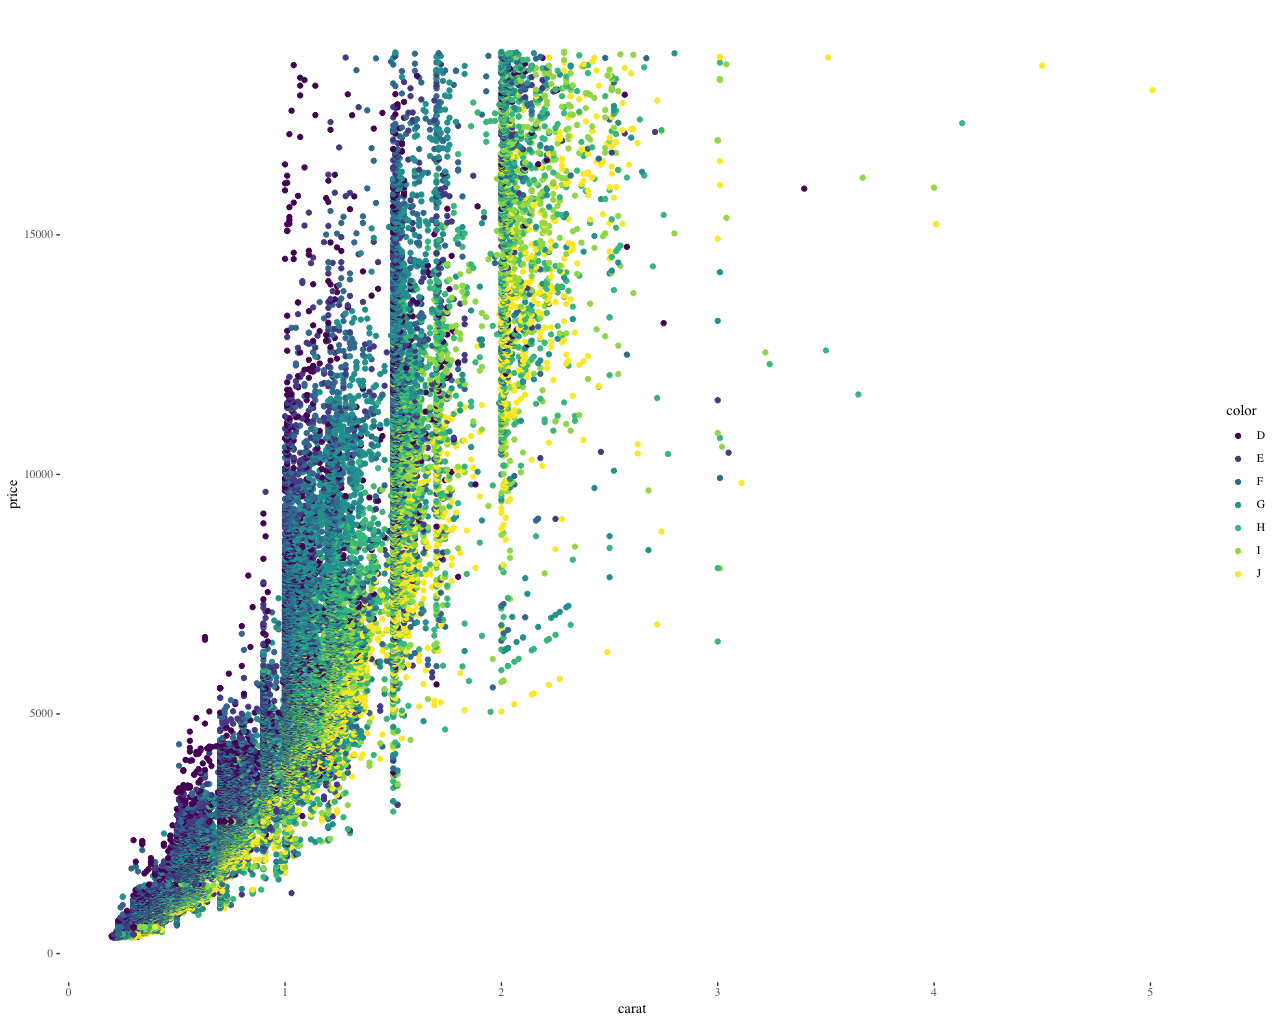
\includegraphics[width=1.0\linewidth]{pic0044}
  \caption{Тема Edward Tufte}
\label{figure0044}
\end{figure}
\FloatBarrier

\begin{figure}[h!]
  \centering
  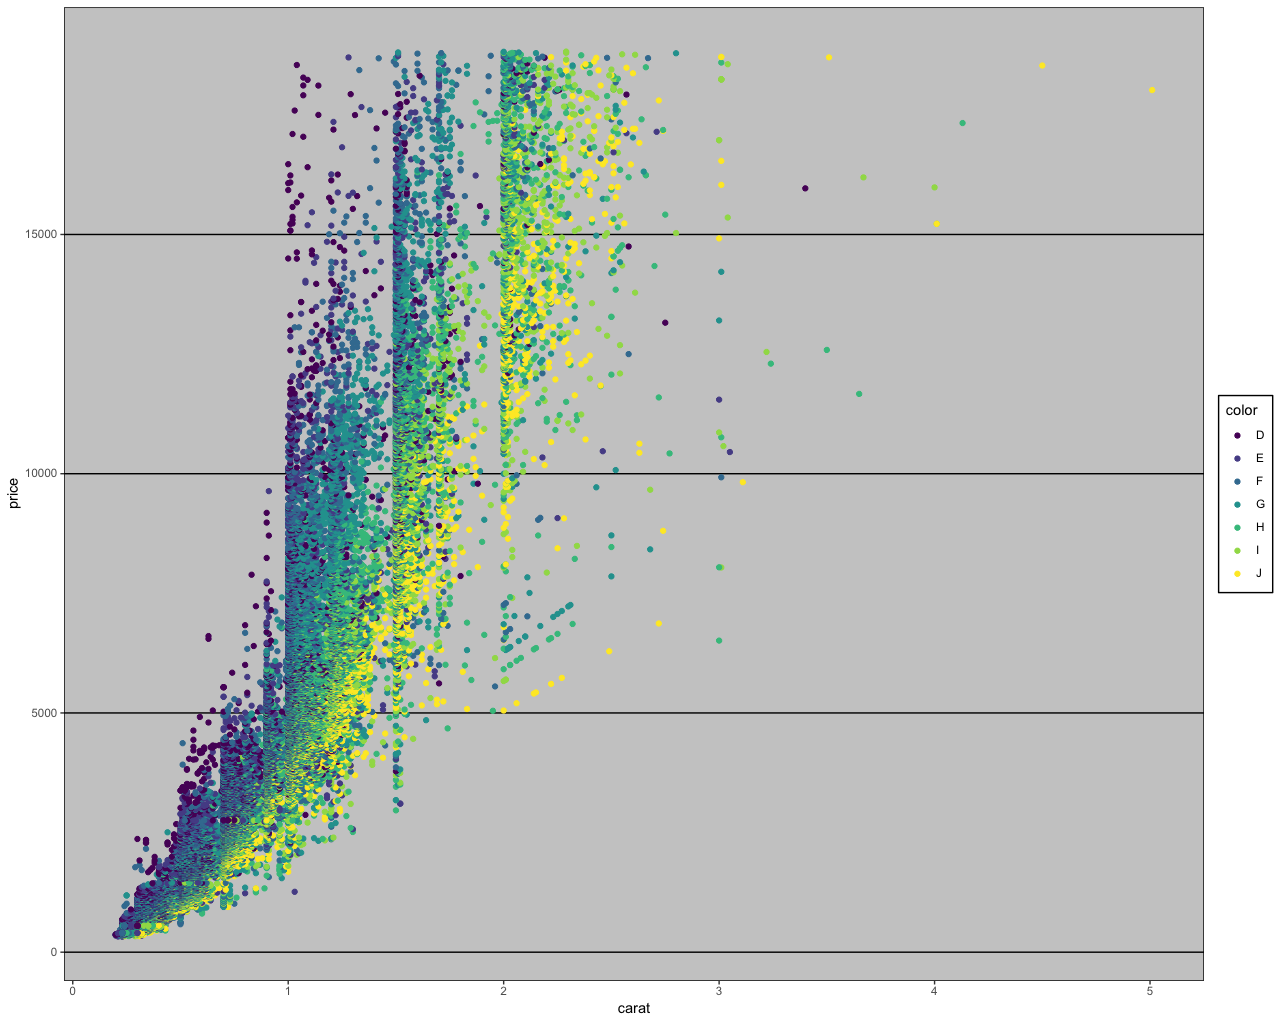
\includegraphics[width=1.0\linewidth]{pic0045}
  \caption{Тема в стил Microsoft Excel}
\label{figure0045}
\end{figure}
\FloatBarrier

\begin{figure}[h!]
  \centering
  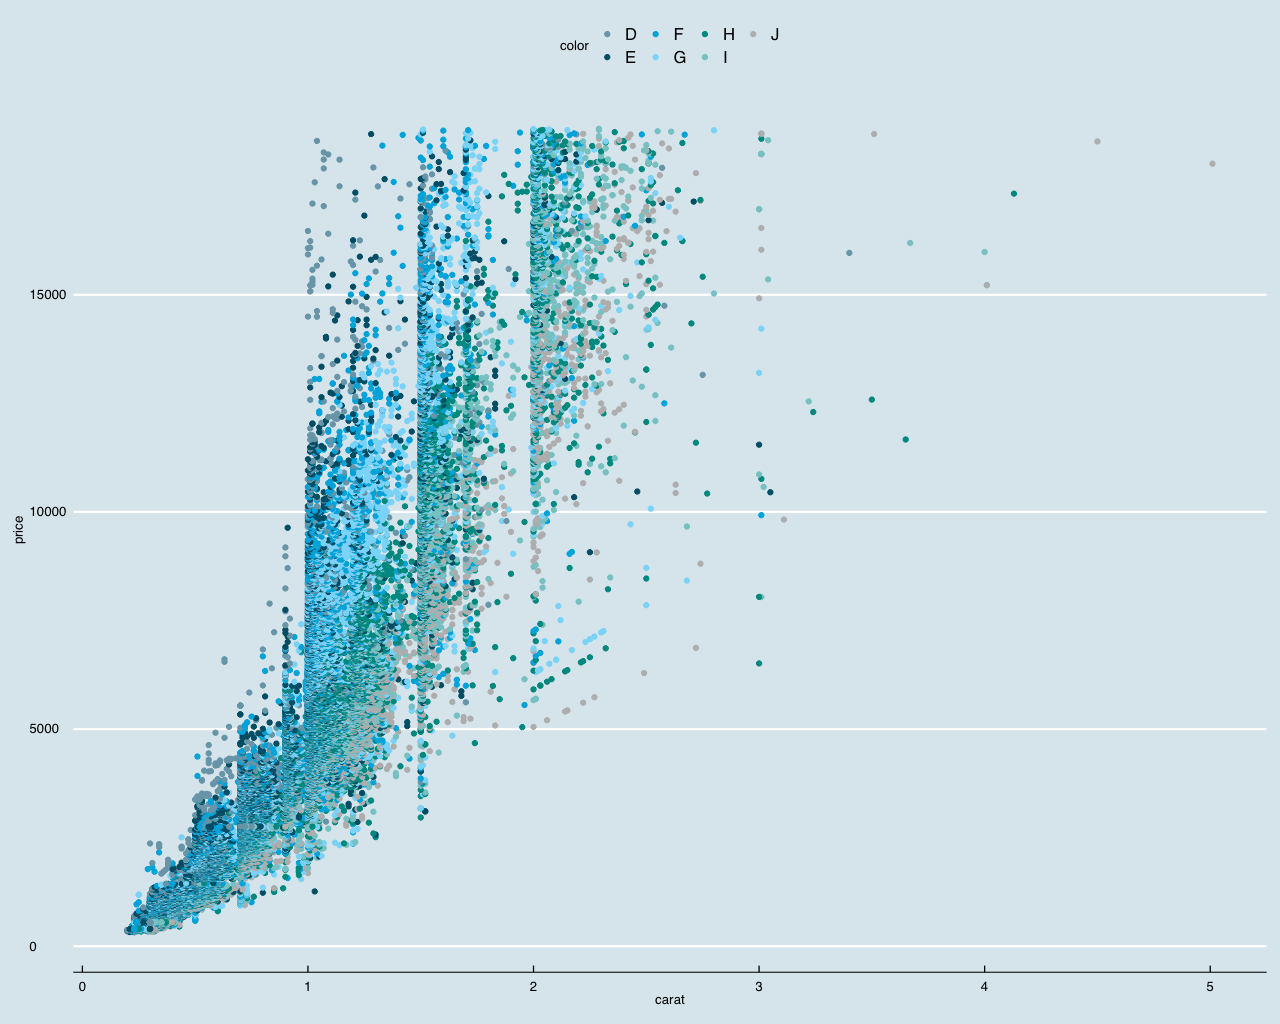
\includegraphics[width=1.0\linewidth]{pic0046}
  \caption{Тема Economist}
\label{figure0046}
\end{figure}
\FloatBarrier

\section{Изследване на случайни величини}

Когато се работи с данни за които няма предварителна информация е от съществено значение да се определи какви са параметрите на вероятностното разпределение. С помощта на пакета Rdice е възможно да се генерират експерименти с различни зарове. Чрез генерирането и статистическото изследване на множество случайни събития се осъществява изследване наречено „Монте Карло метод“.

\begin{lstlisting}[caption=Случайни величини със зарове, label=listing0156]
library(ggplot2)
library(Rdice)

x <- dice.roll(faces=6, dice=1, rolls=100000)

ggplot(data=x$results) + geom_histogram(aes(x=values)) + ggtitle("Single die rolled 100K times.") + xlab("Die Side") + ylab("Outcomes") + scale_x_continuous(breaks=round(seq(min(x$results$values),max(x$results$values),by=0.5)))

x <- dice.roll(faces=6, dice=2, rolls=100000)

ggplot(data=x$results) + geom_histogram(aes(x=(die_1+die_2))) + ggtitle("Two dice rolled 100K times.") + xlab("Dice Sides") + ylab("Outcomes") + scale_x_continuous(breaks=round(seq(min((x$results$die_1+x$results$die_2)),max((x$results$die_1+x$results$die_2)),by=0.5)))

x <- dice.roll(faces=6, dice=6, rolls=100000)
x$results$values = rowSums( x$results[,1:6] )

ggplot(data=x$results) + geom_histogram(aes(x=values)) + ggtitle("Six dice rolled 100K times.") + xlab("Dice Sides") + ylab("Outcomes") + scale_x_continuous(breaks=round(seq(min(x$results$values),max(x$results$values),by=0.5)))

x <- dice.roll(faces=6, dice=10, rolls=100000)
x$results$values = rowSums( x$results[,1:10] )

ggplot(data=x$results) + geom_density(aes(x=values)) + ggtitle("Ten dice rolled 100K times.") + xlab("Dice Sides") + ylab("Outcomes") + scale_x_continuous(breaks=round(seq(min(x$results$values),max(x$results$values),by=0.5)))
\end{lstlisting}

Ако се приеме, че променливата x е резултатът от многократното хвърляне на един математически честен зар, със шест страни, то чрез изчертаване на хистограмата може да се добие представа за характера на случайната величина (Листинг \ref{listing0156}). От изчертаната хистограма ясно се вижда, че случайната величина е дискретна и равномерно разпределена (Фиг. \ref{figure0047}).

\begin{figure}[h!]
  \centering
  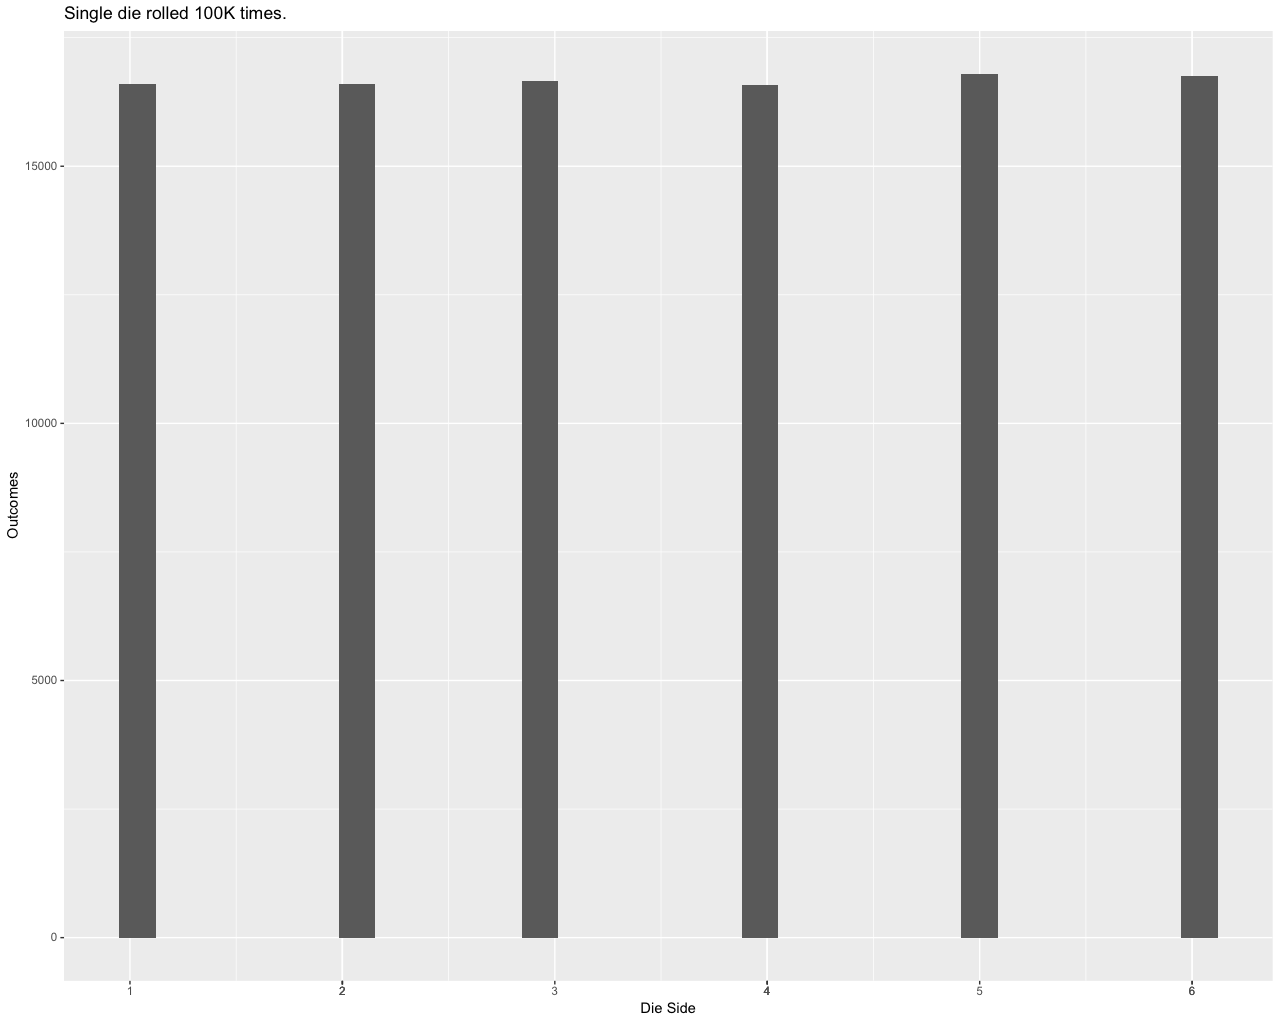
\includegraphics[width=1.0\linewidth]{pic0047}
  \caption{Хистограма на хвърлянията за един зар}
\label{figure0047}
\end{figure}
\FloatBarrier

Когато същият експеримент бъде повторен, но вместо един зар се използват два зара, ясно се различава, че някои събития стават по-малко вероятни от други и разпределението се превръща в триъгълно (Фиг. \ref{figure0048}).

\begin{figure}[h!]
  \centering
  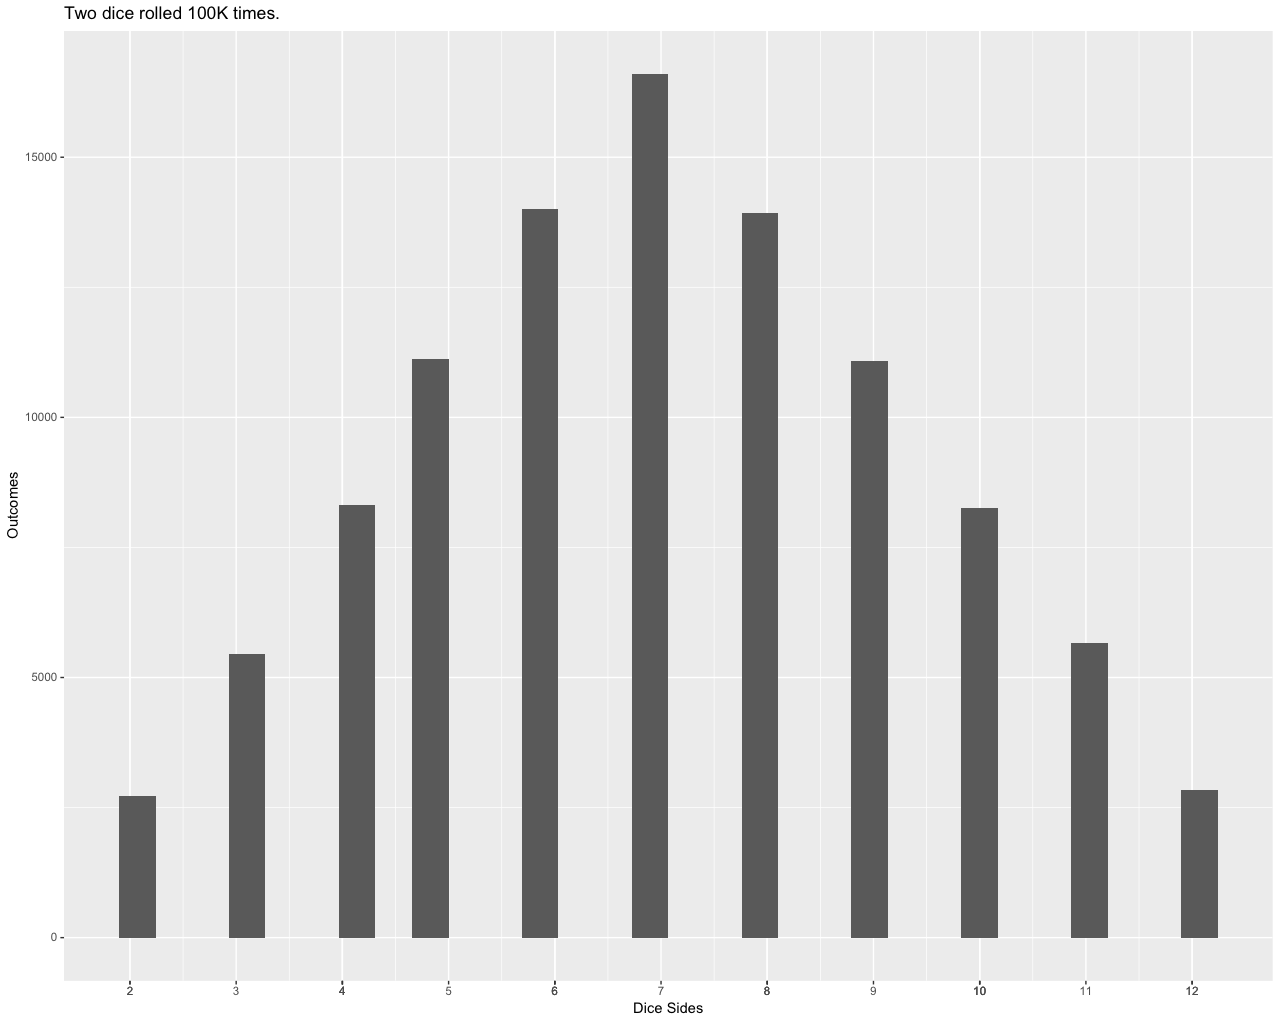
\includegraphics[width=1.0\linewidth]{pic0048}
  \caption{Хистограма на хвърлянията за два зара}
\label{figure0048}
\end{figure}
\FloatBarrier

При шест зара ясно започва да се различава формата на нормалното разпределение (Фиг. \ref{figure0049}).

\begin{figure}[h!]
  \centering
  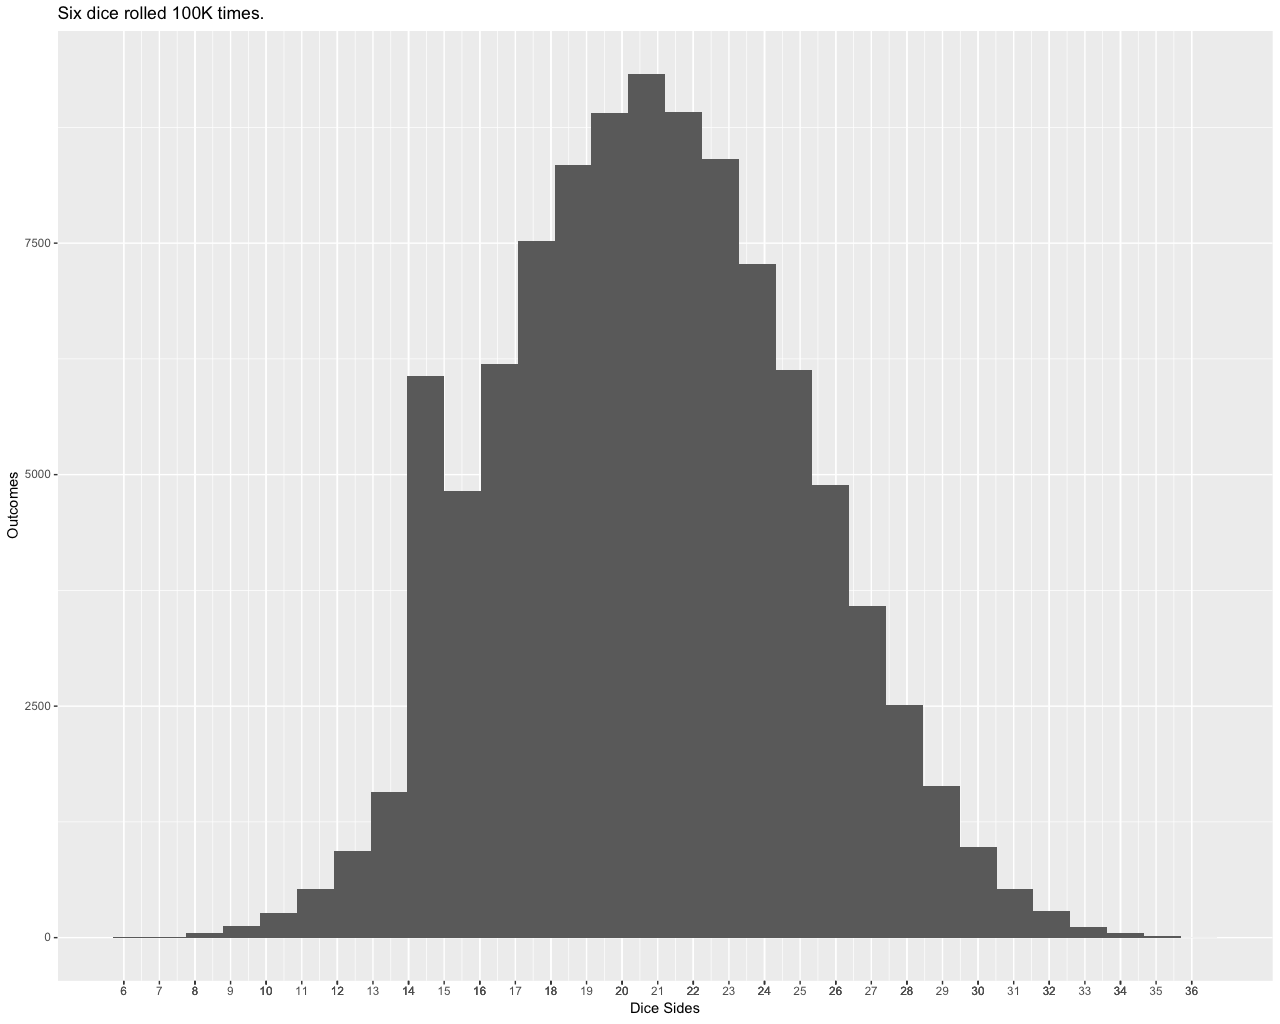
\includegraphics[width=1.0\linewidth]{pic0049}
  \caption{Хистограма на хвърлянията за шест зара}
\label{figure0049}
\end{figure}
\FloatBarrier

При десет зара и изчертаване на плътностна диаграма формата на нормалното вероятностно разпределение е ясно забележима (Фиг. \ref{figure0050}).

\begin{figure}[h!]
  \centering
  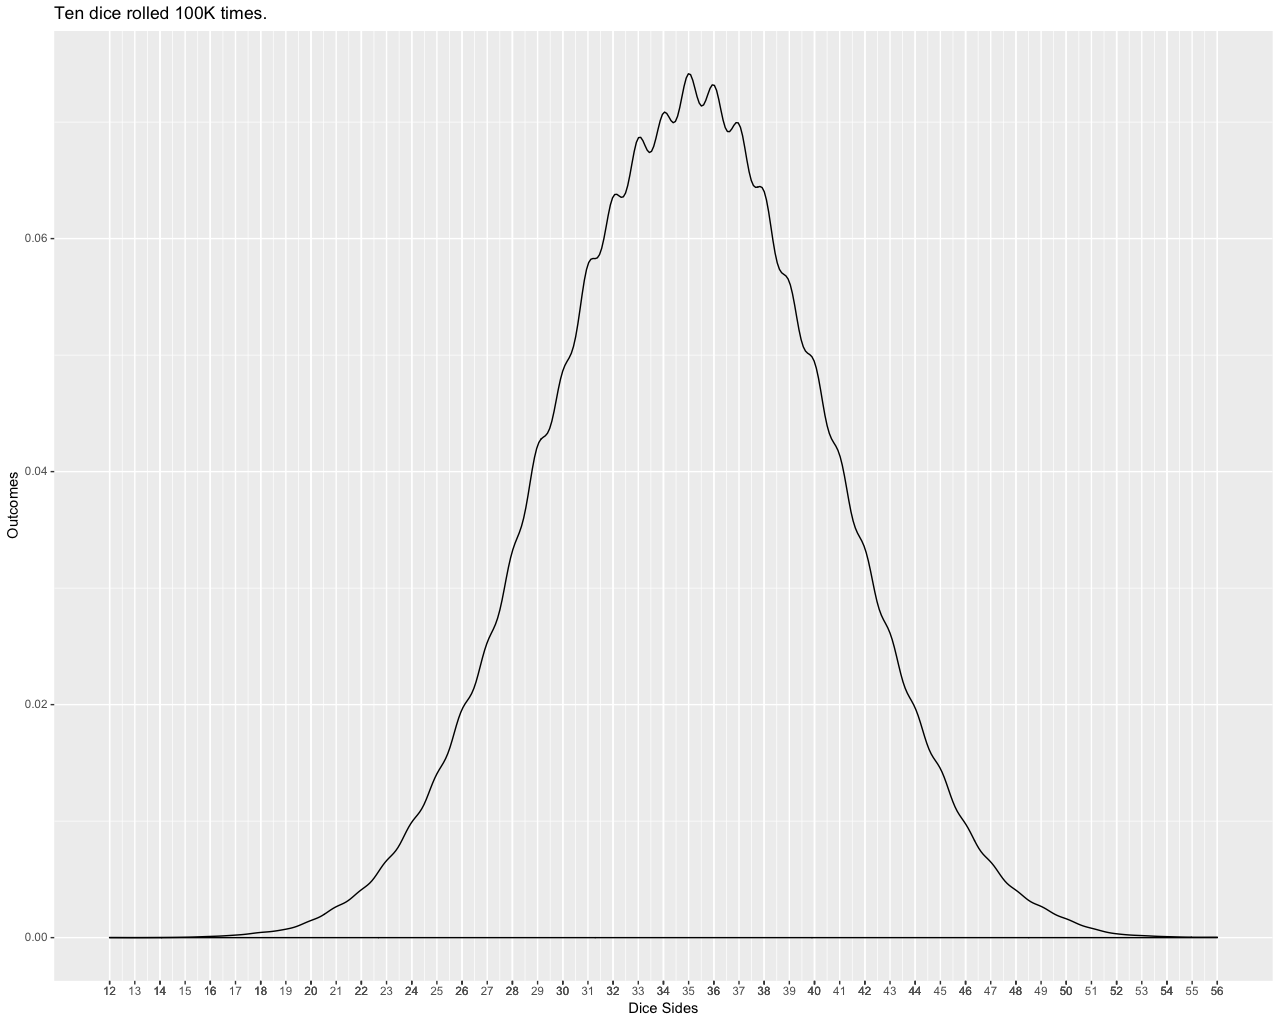
\includegraphics[width=1.0\linewidth]{pic0050}
  \caption{Плътностна диаграма на хвърлянията за десет зара}
\label{figure0050}
\end{figure}
\FloatBarrier

За изследването на една случайна величина, хистограмата и плътностната диаграма носят първоначална ориентировъчна информация за характеристиките на величината.

\section{Вероятностни разпределения}

В реалната практика от статистическия анализ се наблюдават множество случайни величини, които винаги се подчиняват на някакво вероятностно разпределение. Определянето на вероятностното разпределение, към което принадлежи случайната величина има изключително важна роля в адекватното и надеждно извършване на статистическия анализ. След определяне на вероятностното разпределение от съществена важност е и определянето на параметрите, които характеризират разпределението.  

\subsection{Нормално разпределение}

Най-често срещаното в природата и най-използваното в статистическия анализ е нормалното разпределение. Също така, познато е и под названието на Гаусово разпределение (Формула \ref{equation0002}). 

\begin{equation}
pdf(x) = \frac{1}{{\sigma \sqrt {2\pi } }}e^{{{ - \left( {x - \mu } \right)^2 } \mathord{\left/ {\vphantom {{ - \left( {x - \mu } \right)^2 } {2\sigma ^2 }}} \right. \kern-\nulldelimiterspace} {2\sigma ^2 }}}
\label{equation0002}
\end{equation}
\listofequations{Вероятностна функция на нормално разпределение}

Нормалното разпределение се характеризира с два параметъра - средната стойност $\mu$ и стандартно отклонение $\sigma$. Формата на графиката с която се изобразява нормалното разпределение е като камбана. Средната стойност задава къде се намира върхът на камбаната, по оста X, а стандартното отклонение определя широчината на камбаната. 

\begin{lstlisting}[caption=Нормално разпределение, label=listing0157]
library(ggplot2)

values <- rnorm(n=30000, mean=0, sd=0.85)
density <- dnorm( values )
cumulative <- pnorm( values )
quantile <- qnorm( cumulative )

ggplot(data.frame(x=values, y=density)) + aes(x=x, y=y) + geom_line() + labs(x="Normally Distributed Random Values ", y="Density")

ggplot(data.frame(x=values, y=cumulative)) + aes(x=x, y=y) + geom_line() + labs(x="Normally Distributed Random Values ", y="Cumulative Probability")

ggplot(data.frame(x=values, y=quantile)) + aes(x=x, y=y) + geom_line() + labs(x="Normally Distributed Random Values ", y="Quantile")
\end{lstlisting}

В езика R генерирането на нормално разпределени случайни числа става чрез функцията rnorm, която получава параметър за брой числа, средна стойност и стандартно отклонение. Подразбиращата се средна стойност е нула, а подразбиращото се стандартно отклонение е единица. Вероятността дадена стойност да бъде генериране се изчислява с функцията dnorm, която е полезна при изчертаването на плътностната функция (Фиг. \ref{figure0051}).

\begin{figure}[h!]
  \centering
  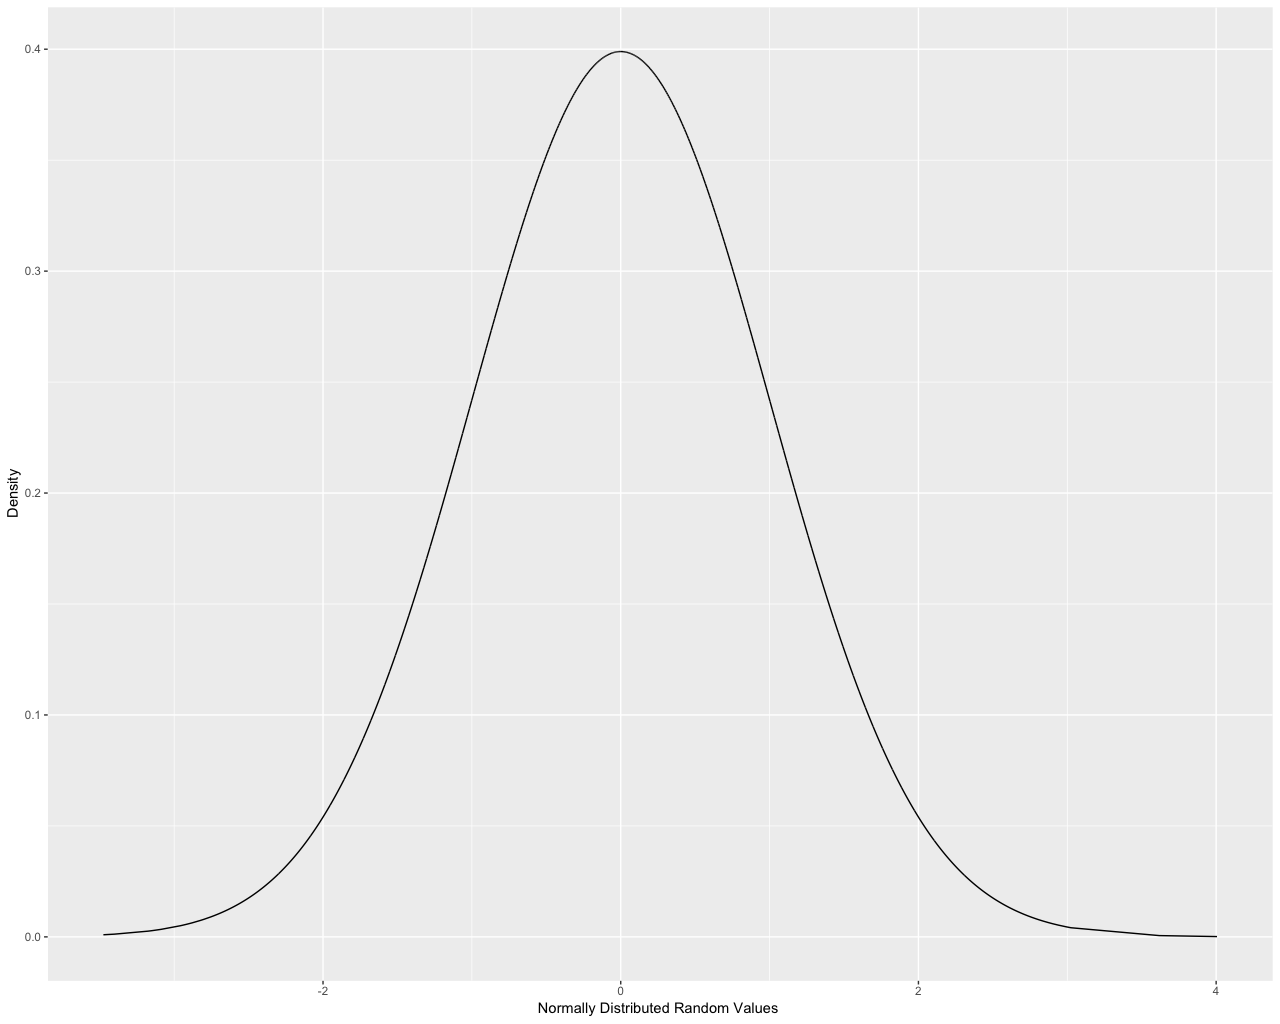
\includegraphics[width=1.0\linewidth]{pic0051}
  \caption{Плътностна функция на нормално разпределение}
\label{figure0051}
\end{figure}
\FloatBarrier

От плътностната функция, чрез интегриране, се получава комулативната функция на разпределението (Формула \ref{equation0003}).

\begin{equation}
cdf(x) = \int_{-\infty}^{a} \frac{1}{{\sigma \sqrt {2\pi } }}e^{{{ - \left( {x - \mu } \right)^2 } \mathord{\left/ {\vphantom {{ - \left( {x - \mu } \right)^2 } {2\sigma ^2 }}} \right. \kern-\nulldelimiterspace} {2\sigma ^2 }}} dx
\label{equation0003}
\end{equation}
\listofequations{Комулативна функция на нормално разпределение}

Смисълът на комулативната функция е, че определя вероятността да се падне число по-малко от зададеното в интервала (Фиг. \ref{figure0052}).

\begin{figure}[h!]
  \centering
  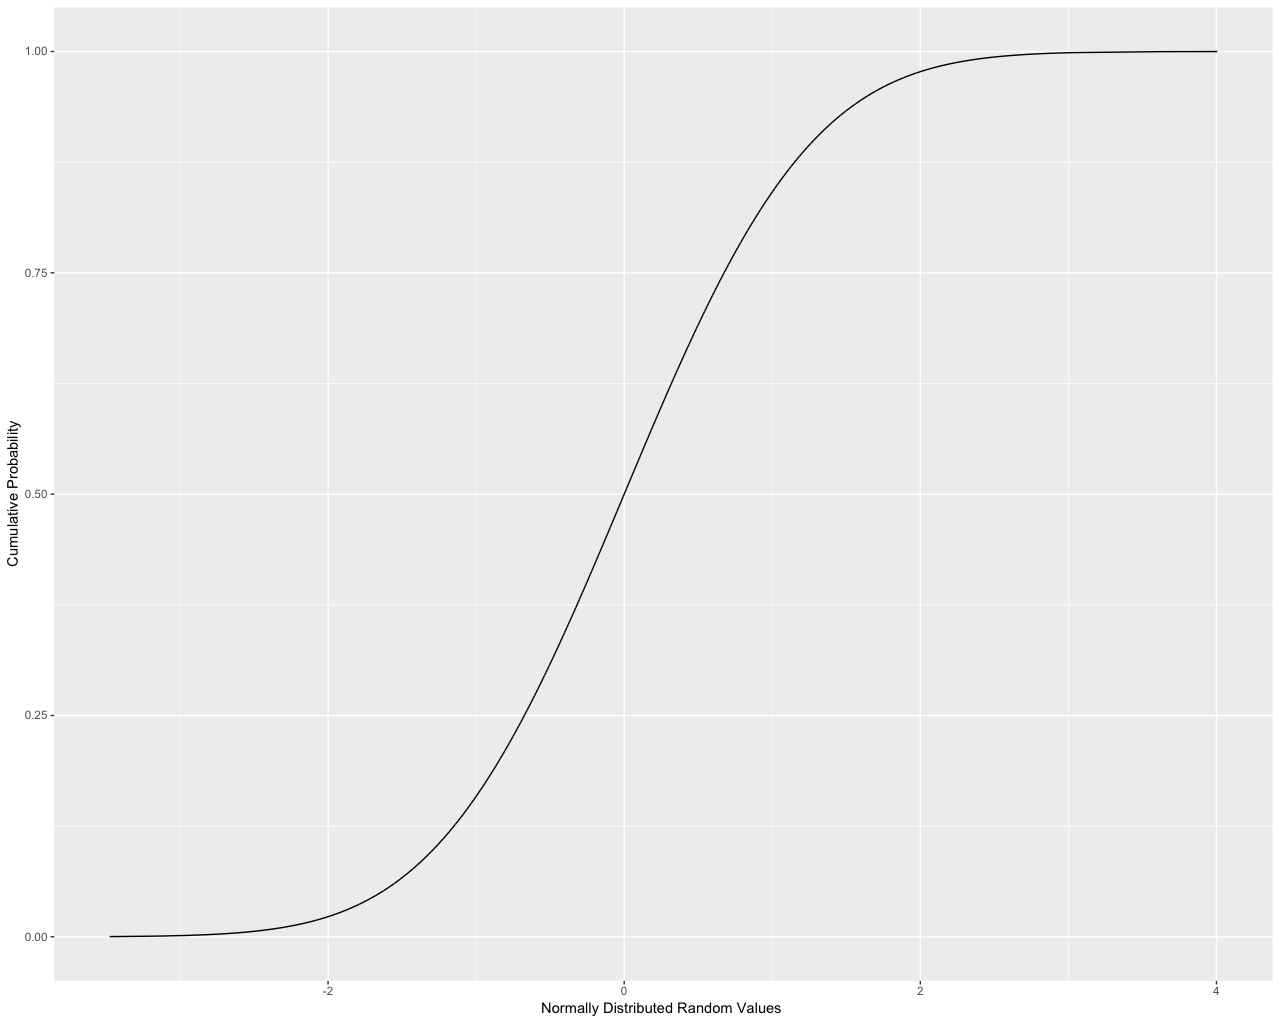
\includegraphics[width=1.0\linewidth]{pic0052}
  \caption{Комулативна функция на нормално разпределение}
\label{figure0052}
\end{figure}
\FloatBarrier

Обратната функция на pnorm е qnorm и тя изчислява квантила, ако е известна комулативната вероятност.

\subsection{Биномно разпределение}

Биномното разпределение (Формула \ref{equation0004}) е добре представено в R с помощта на серия функции по аналогия с функциите за нормално разпределение. 

\begin{equation}
pdf(x) = \binom{n}{x}p^{x}(1-p)^{n-x}
\label{equation0004}
\end{equation}
\listofequations{Вероятностна функция на биномно разпределение}

Където първият множител е биномен коефициент изчисляван по Формула \ref{equation0005}.

\begin{equation}
\binom{n}{x} = \frac{n!}{x!(n-x)!}
\label{equation0005}
\end{equation}
\listofequations{Биномен коефициент}

Параметърът n определя броя опити, а параметърът p задава вероятността за успех при единичен опит. Средната на биномното разпределение е np, а вариацията np(1-p). Когато параметърът n има стойност единица биномното разпределение се трансформира в бернулиево разпределение. 

\begin{lstlisting}[caption=Биномно разпределение, label=listing0158]
library(ggplot2)

values <- rbinom(n=10000, size=7, prob=0.35)
density <- dbinom(x=2, size=7, prob=0.35)
cumulative <- pbinom(q=2, size=7, prob=0.35)
quantile <- qbinom(p=0.15, size=7, prob=0.35)

ggplot(data.frame(x=values)) + aes(x=x) + geom_histogram() + labs(x="Binomial Distributed Random Values ", y="Count")

density
cumulative
quantile
\end{lstlisting}

При биномното разпределение не просто се генерират случайни числа, а се генерират броя на успешните независими бернулиеви експеримента. В езика R за да се генерират биномно разпределени нормални числа се използва функцията rbinom (Листинг \ref{listing0158}). Биномното разпределение е дискретно вероятностно разпределени, тъй като отразява определен брой успешни изходи от експеримент с предварително зададена вероятност за успех. Поради тази причина визуализацията става с помощта на хистограма (Фиг. \ref{figure0053}).

\begin{figure}[h!]
  \centering
  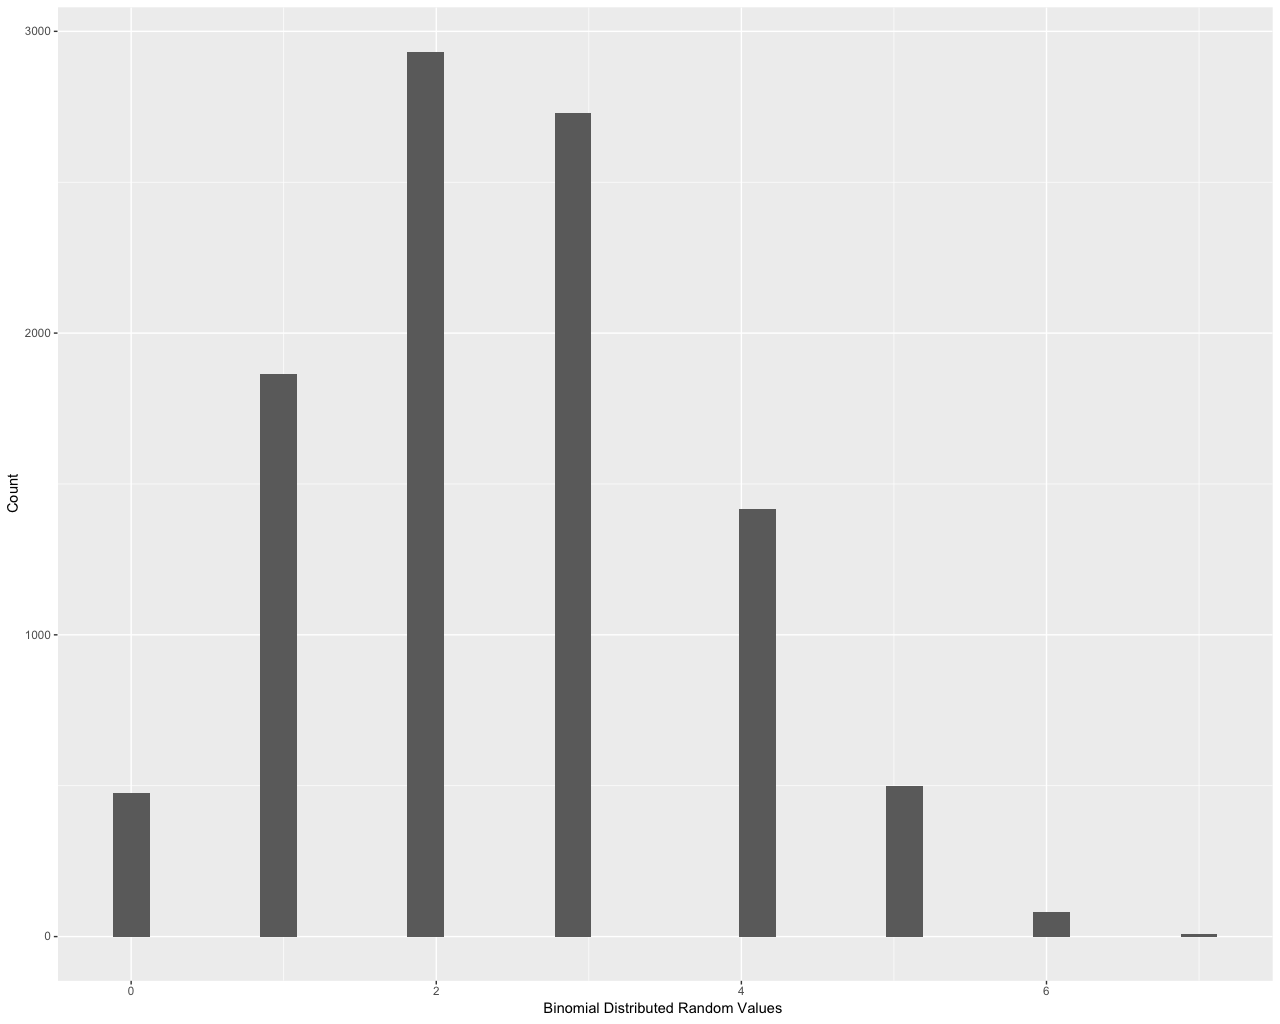
\includegraphics[width=1.0\linewidth]{pic0053}
  \caption{Хистограма на биномно разпределение}
\label{figure0053}
\end{figure}
\FloatBarrier

Освен броя случайни числа които трябва да се генерират към функцията rbinom се подава параметър за броя експерименти и параметър за вероятността на успех при единичен експеримент. При значително увеличаване на броя експерименти биномното разпределение започва да клони към нормално разпределение. 

\begin{equation}
cdf(x) = \sum_{i=0}^{a}\binom{n}{i}p^{i}(1-p)^{n-i}
\label{equation0006}
\end{equation}
\listofequations{Кумулативна функция на биномно разпределение}

С функцията dbinom може да се провери плътността за определена стойност (Формула \ref{equation0006}), а с pbinom кумулативната стойност. И двете функции могат да се използват с вектор от стойности. 

\subsection{Поасоново разпределение}

Популярно в практиката е също и разпределението на Поасон. То има само един параметър $\lambda$, който отразява едновременно средната стойност и дисперсията (Формула \ref{equation0007}). 

\begin{equation}
pdf(x) = \frac{\lambda^{x}e^{-\lambda}}{x!}
\label{equation0007}
\end{equation}
\listofequations{Вероятностна функция на поасоново разпределение}

Разпределението е дискретно и намира приложение при случайни променливи, които отразяват случването на брой случайни събития в зададен интервал от време. 

\begin{equation}
cdf(x) = \sum_{i=0}^{a}\frac{\lambda^{i}e^{-\lambda}}{i!}
\label{equation0008}
\end{equation}
\listofequations{Кумулативна функция на поасоново разпределение}

Както и при повечето други вероятностни разпределения, това също започва да клони към нормалното разпределени когато параметърът $\lambda$ нарасне до големи стойности. 

\begin{lstlisting}[caption=Разпределение на Поасон, label=listing0159]
library(ggplot2)

values <- rpois(n=1000, lambda=0.8)
density <- dpois(x=2, lambda=0.8)
cumulative <- ppois(q=2, lambda=0.8)
quantile <- qpois(p=0.75, lambda=0.8)

ggplot(data.frame(x=values)) + aes(x=x) + geom_histogram() + labs(x="Poisson Distributed Random Values ", y="Count")

density
cumulative
quantile
\end{lstlisting}

Визуализацията на поасоновото разпределение става с помощта на хистограма (Фиг. \ref{figure0054}).

\begin{figure}[h!]
  \centering
  \includegraphics[width=1.0\linewidth]{pic0054}
  \caption{Хистограма на поасоново разпределение}
\label{figure0054}
\end{figure}
\FloatBarrier

С функцията dpois може да се провери плътността за определена стойност (Формула \ref{equation0008}), а с ppois кумулативната стойност. И двете функции могат да се използват с вектор от стойности. 

\subsection{Други разпределения}

Пакетът R предлага богат набор от вероятностни разпределения (Фиг. \ref{figure0055}). Една част от тези разпределения са широко използвани, други не чак толкова.

\begin{figure}[h!]
  \centering
  \includegraphics[width=1.0\linewidth]{pic0055}
  \caption{Списък с най-използваните вероятностни разпределения}
\label{figure0055}
\end{figure}
\FloatBarrier

\section*{Заключение}

Визуалното представяне на числените данни повишава степента за възприемане на представяната информация. Колкото по-големи са възможностите на пакетите за визуално представяне, толкова повече възможности биха имали хората работещи с информация и нейното представяне пред широка аудитория. При анализа на случайни величини, визуализацията с хистограма и плътностна функция може да даде най-груба първоначална представа за параметрите на случайната величина. Информация, която може да бъде изключително полезна при избора на по-сложни методи за статистически анализ. От своя страна, визуализацията на случайностите най-удачно се представя, чрез някои от най-използваните вероятностни разпределения. 


\newpage
\chapter{Статистическа обработка на данните}
\label{chapter09}

Статистическата обработка на данни се състои основно от два вида статистика – описателна статистика и сравнителна статистика. При описателната статистика се изчисляват определени параметри описващи характеристики на събраните данни, докато при сравнителната статистика се извършва сравнение между някои от описателните параметри на данните. 

\section{Описателна статистика}

Параметрите при описателната статистика основно са свързани с някакво централно групиране на данните и някакво разпръскване (дисперсия) около централното групиране. Параметри за централно групиране са средната стойност, медианата и модата, а параметри за разпръскване са дисперсията и стандартното отклонение.

\begin{lstlisting}[caption=Генериране на извадка от случайни числа, label=listing0160]
v1 <- round( rnorm(100, mean=62, sd=72) )

v2 <- v1

v2[sample(x=1:100, size=15, replace=FALSE)] <- NA

w1 <- 1 / sample(x=1:100, size=100, replace=TRUE)
\end{lstlisting}

За да бъдат илюстрирани възможностите на R за пресмятане на описателни статистики се използва извадка от 100 нормално разпределени случайни числа (Листинг \ref{listing0160}). Често в реалната практика данните съдържат липсващи измервания. При такава ситуация трябва да се вземат допълнителни мерки за пресмятане на описателните статистики. Функцията sample в R позволява на случаен принцип част от стойностите в определен вектор да бъдат избрани на случаен принцип, при равномерно вероятностно разпределение. Тази възможност се използва за замяна на 15\% от генерираните данни с липсваща стойност (Листинг \ref{listing0160}). Параметърът replace указва дали определено число може да бъде избрано повторно или не.

\subsection{Средна стойност}

Средната стойност е най-често използваната статистика и представлява сумата от стойностите разделена на общия брой стойности (Листинг. \ref{listing0161}).

\begin{lstlisting}[caption=Средна стойност, label=listing0161]
sum(v1) / length(v1)

mean( v1 )

mean( v2 )

mean(v2, na.rm=TRUE)
\end{lstlisting}

Когато липсват стойности при проведените измервания е невъзможно да се изчисли средната стойност без да се вземе решение как да се обработят липсващите числа. Има различни подходи за обработката на липсите, като интерполация или премахване. Независимо кой подход бъде избран, то той неизбежно води до внасяне на допълнителна грешка при пресмятанията. Ако бъде извършена интерполация, то съседните измервания биха внесли грешка в липсващите стойности. Ако бъдат премахнати липсващите измервания, то размерът на извадката намалява, а от там се увеличава и неточността на последващите пресмятания. 

В някои ситуации отделните измерени стойности имат различна тежест и се налага те да участват с различен коефициент при пресмятането на средната стойност (Листинг \ref{listing0162}). Такава е ситуацията когато се пресмята бал за прием в учебно заведение. Различните компоненти формиращи бал на всеки кандидат участват с различна тежест.

\begin{lstlisting}[caption=Претеглена средна стойност, label=listing0162]
weighted.mean(x=v1, w=w1)
\end{lstlisting}

\subsection{Минимална стойност, максимална стойност, медиана и мода}

В практиката често от значение е диапазонът в който се разпростират данните. В програмния пакет R този диапазон лесно се установява с функциите min и max (Листинг \ref{listing0163}).

\begin{lstlisting}[caption={Минимум, максимум, медиана и мода}, label=listing0163]
min( v1 )

max( v1 )

median( v1 )

# Mode calculation.
unique(v1)[ which.max( tabulate(match(v1,unique(v1)) ) ) ]
\end{lstlisting}

Един от основните недостатъци на средната стойност е, че при наличието на екстремално различни отделни измервания силно могат да повлияят върху общото пресмятане на средната стойност. Поради тази причина в практиката много често се използва медианата, а не средната стойност (Листинг \ref{listing0163}). За да се пресметне медианата данните се сортират. При нечетен брой стойности медианата е стойността на средния елемент. При четен брой стойности медианата е средно аритметично между двата елемента в средата. 

Модата е параметър, който отразява най-често срещаната стойност в множеството от данни. Освен числена стойност модата може да има и символна стойност, според характера на самите данни. В програмния пакет R няма функция, която да изчислява модата, но тя лесно може да се пресметне с комбинация от извикването на други функции (Листинг \ref{listing0163}).

\subsection{Дисперсия и стандартно отклонение}

След като бъде установено някакво централно групиране в данните е от съществено значение по какъв начин данните са разпръснати около това централно групиране. Изчисляването на дисперсията спомага за изследване на разпръскването (Листинг \ref{listing0164}). Дисперсията се изчислява като сума от квадрата на разликите между всяка стойност и средната, разделена на броя стойности минус едно. 

\begin{lstlisting}[caption=Дисперсия и стандартно отклонение, label=listing0164]
sum( (v1-mean(v1))^2 ) / (length(v1) - 1)

var( v1 )

sqrt( var(v1) )

sd( v1 )
\end{lstlisting}

Основен недостатък на дисперсията е, че се изчислява с повдигане на втора степен и полученият резултат е несравним с оригиналните измервания. Примерно при серия измервания в метри резултатът от изчислението на дисперсията би имал смисъла на квадратни метри. За да бъдат сравними стойностите е достатъчно дисперсията да се подложи на корен квадратен, което коригира резултата получен с повдигане на втора степен. Резултатът от квадратния корен на дисперсията се нарича стандартно отклонение (Листинг \ref{listing0164}).

\subsection{Квантили и обобщение}

Квантилите определят каква част от измерените стойности попадат в определен процент от вероятностното разпределение (Листинг \ref{listing0164}).

\begin{lstlisting}[caption=Квантили и обобщение, label=listing0165]
quantile(v1, probs=c(0.1, 0.2, 0.3, 0.4, 0.5, 0.6, 0.7, 0.8, 0.9))
#  10%   20%   30%   40%   50%   60%   70%   80%   90% 
#-28.0  -0.4  19.0  41.6  66.5  84.4 110.6 121.8 150.2 

summary( v1 )
\end{lstlisting}

Програмният пакет R предоставя и обобщаваща функция за описателните статистики наречена summary и тя визуализира стойностите за минимална, максимална, медиана, средна, първи и трети квантил.

\section{Сравнителна статистика}

Когато се работи с две или повече случайни променливи от ползва идва апарата на сравнителната статистика. Целта е да се изследва връзката между тези променливи. За променливи от едно и също измерване най-често се използват корелацията и ковариацията, а за сравнение на средни T-тест и ANOVA. 

\subsection{Ковариация и корелация}

Корелационният коефициент е число в интервала -1 до +1 и показва възможността за наличие на взаимна връзка между две случайни променливи. Важно е да се отбележи, че корелационният коефициент не гарантира наличие на взаимна връзка, а само указва, че такава връзка е възможна. 

\begin{lstlisting}[caption=Ковариация и корелация, label=listing0166]
library(ggplot2)

cor(economics$psavert, economics$pce)

# Correlation formula.
sum((economics$psavert-mean(economics$psavert)) * (economics$pce-mean(economics$pce))) / ((nrow(economics)-1) * sd(economics$psavert) * sd(economics$pce))

cor(economics[, c("pce","psavert","uempmed","unemploy")])

cov(economics$psavert, economics$pce)

cov(economics[, c("pce","psavert","uempmed","unemploy")])

# Correlation is a covariance divided by the standard deviation.
identical(cov(economics$psavert,economics$pce),cor(economics$psavert,economics$pce)*sd(economics$psavert)*sd(economics$pce))
\end{lstlisting}

В пакета ggplot2 множеството от данни economics дава идеална възможност да се демонстрира концепцията за корелация и ковариация (Листинг \ref{listing0166}). Колоната psavert отразява индивидуалното спестовно ниво, а колоната pce индивидуалните разходи. При относително еднакво ниво на доходите, чисто интуитивно е ясно, че който харчи повече би следвало да спестява по-малко. Това ще рече, че когато едната стойност нараства другата стойност ще намалява и това има смисъла на отрицателна корелационна връзка. В демонстрирания пример корелационният коефициент е -0.7928546 и отразява точно факта за възможно наличие на относително силна отрицателна корелационна връзка. 

\begin{equation}
r_{xy} = \frac{\sum_{i=1}^{n}(x_i-\bar{x})(y_i-\bar{y})}{(n-1)s_xs_y}
\label{equation0009}
\end{equation}
\listofequations{Корелационен коефициент}

Корелационният коефициент се пресмята като сума от разликите между множителите на отделните измервания в разлика от средната стойност, разделена на умножението между стандартните отклонения на двете променливи с броя измервания минус единица (Формула \ref{equation0009}). При стойност близка до +1 е възможна силна положителна корелационна връзка, при стойност близка до -1 е възможна силна отрицателна корелационна връзка, а при стойност близка до 0 наличието на корелационна връзка е много малко вероятно. 

Когато корелацията се смята между повече от две случайни променливи резултатът е корелационна матрица (Листинг \ref{listing0166}). При корелационната матрица е показана възможната връзка между всяка двойка променливи. 

\begin{equation}
v_{xy} = \frac{1}{n-1}\sum_{i=1}^{n}(x_i-\bar{x})(y_i-\bar{y})
\label{equation0010}
\end{equation}
\listofequations{Ковариационен коефициент}

Ковариацията е подобна на корелацията, като разликата е, че стойностите не са нормирани (Формула \ref{equation0010}). Може да се приеме като аналогия между дисперсията и стандартното отклонение (Листинг \ref{listing0166}). Ковариацията може да бъде голямо отрицателно число или голяма положително число. В посочения пример ковариацията е със стойност -8359.069, при съответната ковариационна матрица. 

Както при описателните статистики, при ковариацията и корелацията липси в измерванията възпрепятстват изчисляването на крайните стойности. 

\subsection{Тест на Стюдънт}

От сравнителната статистика t-теста (или тест на Стюдънт) е един от най-разпространените подходи за сравнение на средните стойности между две извадки. 

\begin{lstlisting}[caption=Тестово множество за бакшиши, label=listing0167]
library(reshape2)

head(tips)
\end{lstlisting}

За илюстриране на възможностите, които R предлага при пресмятането на t-теста е подходящо да се използва множеството данни за бакшиши (Листинг \ref{listing0167}).

\subsubsection{Тест на една извадка}

При тестването на една извадка теста се прилага за определяне на средната стойности и съответният доверителен интервал. От съществено значение е данните да са нормално разпределение което означава, че имат конкретна средна стойност и конкретно стандартно отклонение. Ако тестваната стойност попада в доверителния интервал, то може да се заключи, че това е действителната средна стойност. В противен случай не може да се приеме, че предположената средна стойност е действителната средна стойност. 

\begin{lstlisting}[caption=Тест на единична извадка, label=listing0168]
t.test(tips$tip, alternative="two.sided", mu=3.50)

# 	One Sample t-test
# 
# data:  tips$tip
# t = -5.6642, df = 243, p-value = 4.161e-08
# alternative hypothesis: true mean is not equal to 3.5
# 95 percent confidence interval:
#  2.823799 3.172758
# sample estimates:
# mean of x 
#  2.998279 
\end{lstlisting}

При проверката дали средната стойност на бакшишите е \$3.5 $t$-тестът завършва с отчет за пресметнатите стойности (Листинг \ref{listing0168}), което включва - $t$ статистиката, степените на свобода и $p$ стойността. Също така е представена информация за 95 процентният доверителен интервал и информация за средната стойност на изследваната променлива. Постигнатата p стойност означава, че нулевата хипотеза трябва да бъде отхвърлена. Това води до заключението, че средната стойност на бакшишите не може да е \$3.5. Нулевата хипотеза е това, което се смята за истина (в примера това е средна стойност е равна на \$3.5). 

\begin{equation}
t = \frac{\bar{x}-\mu_0}{s_{\bar{x}}/\sqrt{n}}
\label{equation0011}
\end{equation}
\listofequations{T-статистика}

T-статистиката се смята по формула \ref{equation0011} и има смисъла на отношение между разликата от пресметнатото средно ($\bar{x}$) и предположеното средно ($\mu_0$), а като делител е стандартната грешка на пресметнатото средно ($s_{\bar{x}}/\sqrt{n}$). В уравнението $s_{\bar{x}}$ има смисъла на стандартно отклонение, а $n$ е броят на наблюденията. 

\begin{figure}[h!]
  \centering
  \includegraphics[width=1.0\linewidth]{pic0056}
  \caption{Т-статистика за бакшиши}
\label{figure0056}
\end{figure}
\FloatBarrier

Когато предположената средна стойност е вярна очакването е $t$-статистиката да попада в интервала от две стандартни отклонения, около средната стойност (Фиг. \ref{figure0056}). 

\begin{lstlisting}[caption=Визуализация на t-разпределение, label=listing0169]
library( ggplot2 )

# Generation of t-distributed random values.
values <- rt(10000, df = NROW( tips ) - 1)

# T-statistics calculation.
t <- t.test(tips$tip, alternative="two.sided", mu=3.50)

# Visualization.
ggplot(data.frame(x=values)) + geom_density(aes(x=x), fill="grey", color="grey") + geom_vline(xintercept=t$statistic) + geom_vline(xintercept=mean(values) + c(-2, 2) * sd(values), linetype=2)
\end{lstlisting}




\newpage
\chapter{Приближени пресмятания - подходи, методи, алгоритми}
\label{chapter10}
\thispagestyle{empty}

В изчислителната математика се открояват две основни направления – точните числени пресмятания и приближените числени пресмятания\index{приближени пресмятания}. Точни числени пресмятания\index{точни числени методи} се извършват в ситуации в които обемът на задачата позволява изчисленията да се осъществят в приемлив интервал от време. В реалната практика често поставяните задачи значително нарастват като обем и тяхното пресмятане с точени числени методи става неприемливо по отношение на нужното време за пресмятане. В такива ситуации се прибягва до множеството разработени методи за приближени пресмятания\index{приближени числени методи}. По отношение на програмния продукт R, ще бъдат разгледани някои от най-популярните методи за приближени числени пресмятания, а именно Монте-Карло симулации, генетични алгоритми и изкуствени невронни мрежи.

\section{Монте-Карло методи}

В средата на XX век, във връзка с разработването на първите ядрени оръжия, са разработени група методи за приближени пресмятания, които залагат на способ за генериране на голямо количество случайни числа и последващата им статистическа обработка. Монте-Карло методите\index{Монте-Карло методи} намират най-голямо приложение в оптимизационни задачи, числено интегриране и генериране на семпли за специфични вероятностни разпределения. Монте-Карло методите могат да се използват за решаването на всяка задача, която има представяне в термините на вероятности и статистика. 

Има вариации в реализацията на Монте-Карло методите, но те в общия случай следват няколко добре дефинирани стъпки:

1. Определяне на област от допустими стойности;

2. Генериране на извадка от случайни числа в предварително дефинираната област;

3. Извършване на точни пресмятания с така генерираните случайни числа;

4. Обобщаване на резултатите от извършените пресмятания.

\begin{figure}[h!]
  \centering
  \includegraphics[width=0.8\linewidth]{pic0060}
  \caption{Пресмятане на числото $\pi$ с Монте-Карло метод}
\label{figure0060}
\end{figure}
\FloatBarrier

Един от най-популярните примери за Монте-Карло пресмятане е приближеното изчисление на числото $\pi$ (Фиг. \ref{figure0060}). За тази цел една четвърт от окръжност се представя с обгръщащия я квадрат. Съотношението между площите на квадрата и на четвъртината окръжност е $\pi/4$. За да се апроксимира стойността на числото $\pi$ с Монте-Карло метод се изпълняват следните стъпки:

1. Изчертаване на квадрат и четвъртина окръжност вписана в него;

2. Генериране на случайни равномерно разпределени числа, като координати (x,y двойки) в описаната допустима област;

3. Изброяване на точките с координати x,y които са на разстояние 1 от центъра на четвърт окръжността; 

4. Съотношението между точките в четвърт окръжността и общия брой точки е $\pi/4$, което умножено по 4 дава приближена стойност за числото $\pi$. 

При тази процедура за приближено пресмятане е важно да се вземат под внимание два много важни фактора:

1. Ако генерираните случайни числа не са равномерно разпределени, това ще доведе до невярна апроксимация за търсената стойност;

2. Генерирането на малък брой координати за точки в дефиниционната област води до ниско надеждна стойност за апроксимация, което означава, че колкото по-голям обем е извадката от случайни числа, толкова по-надеждни резултати за апроксимация.

\begin{lstlisting}[caption=Монте-Карло пресмятане, label=listing0175]
library( MonteCarlo )

mode <- function(x) {
	values <- unique(x)
	return( values[which.max(tabulate(match(x, values)))] )
}

experiment <- function(n, d){
	x <- sample(6,n,TRUE)

	for(i in 2:d) {
		x <- x + sample(6,n,TRUE)
	}

	return( list("mean"=mean(x), "median"=median(x), "mode"=mode(x)) )
}

result <- MonteCarlo(func=experiment, nrep=1000, param_list=list("n"=c(10, 50, 100, 150, 200),"d"=c(1,2,6)))

summary( result );

MakeTable(output=result, rows=c("d"), cols=c("n","list"), digits=2, include_meta=FALSE)
\end{lstlisting}

Към програмния продукт R е създаден отделен пакет (автор Christian Hendrik Leschinski) за извършване на Монте-Карло пресмятания, наречен „MonteCarlo“ (Листинг \ref{listing0175}). 

За демонстрация на възможностите, които R дава при Монте-Карло симулации е представено сравнение между средната, медианата и модата за вероятностно разпределение на сумата от $n$ зара. Тъй като R не предлага функция за пресмятане на мода е необходимо тази функция да бъде предварително дефинирана (Листинг \ref{listing0175}).

В пакета $MonteCarlo$\index{Монте-Карло методи} основно се използват две функции - $MonteCarlo$ и $MakeTable$. Функцията $MonteCarlo$ има за основна задача генерирането на множеството експерименти в процеса на симулацията. Най-важният параметър за тази функция е функционален обект, който описва единичен експеримент. В програмния език R функционалните обекти по своята същност представляват потребителски дефинирани функции. В предложения пример функционалният обект се нарича $experiment$, а функцията която представлява получава два входни параметъра $n$ и $d$. Потребителят на пакета $MonteCarlo$ сам може да избира какъв брой параметри да има функцията за единичен експеримент. В настоящия пример $n$ определя броят случайни числа, които да бъдат генерирани (размер на случайната извадка), а $d$ определя колко зара ще участват във формирането на крайния резултат. При предишни примери бе показано, че вероятностното разпределение на един зар е равномерно, на два зара триъгълно, а при достатъчно много зарове разпределението клони към нормалното. В този пример се разглеждат разликите между средната, медианата и модата за 1, 2 и 6 зара.

Към функцията за единичен експеримент има следните изисквания: 1. Аргументите а бъдат скаларни стойности; 2. Върнатата стойност от функцията да бъде списък с именувани или неименувани скаларни стойности. Потребителската функция за единичен експеримент се изпълнява в текущото работно пространство и поради тази причина всички нужни библиотеки, променливи с данни и помощни функции трябва да са заредени предварително. 

Вторият важен аргумент на функцията $MonteCarlo$ е $param_list$ и трябва да изпълнява следните изисквания: 1. Трябва да е списъчна структура; 2. Елементите на списъка трябва да са именувани и имената да съответстват на имената използвани за параметри в потребителската функция за единичен експеримент; 3. Всеки елемент в списъка е вектор със скаларни стойности; 4. Списъкът съдържа точно толкова на брой елементи, колкото са параметрите на потребителската функция за единичен експеримент. 

Последният задължителен аргумент на функцията $MonteCarlo$ е $nrep$ и той определя колко пъти ще бъде изпълнен Монте-Карло експериментът. В представения пример (Листинг \ref{listing0175}) се изпълняват хиляда повторения за три възможни комбинации от зарове, при пет различни броя за хвърлянето на тези зарове, а именно 10, 50, 100, 150 и 200. 

\begin{table}[h]
\centering
\resizebox{ 1 \textwidth}{!}{%
\begin{tabular}{ rrrrrrrrrrrrrrrrrrr }
\hline\hline\\\\
 list && \multicolumn{ 5 }{c}{ mean } &  & \multicolumn{ 5 }{c}{ median } &  & \multicolumn{ 5 }{c}{ mode } \\ 
d/n &  & 10 & 50 & 100 & 150 & 200 &  & 10 & 50 & 100 & 150 & 200 &  & 10 & 50 & 100 & 150 & 200 \\ 
 &  &  &  &  &  &  &  &  &  &  &  &  &  &  &  &  &  &  \\ 
1 &  & 10.50 & 10.48 & 10.49 & 10.50 & 10.50 &  & 10.52 & 10.50 & 10.48 & 10.50 & 10.52 &  & 10.48 & 10.50 & 10.42 & 10.49 & 10.53 \\ 
2 &  &  7.01 &  7.00 &  7.00 &  7.01 &  6.99 &  &  7.02 &  7.01 &  7.00 &  7.00 &  7.00 &  &  7.03 &  7.04 &  6.98 &  6.98 &  6.99 \\ 
6 &  & 20.94 & 21.03 & 21.00 & 21.01 & 21.00 &  & 20.90 & 21.01 & 20.99 & 21.00 & 21.00 &  & 20.86 & 20.98 & 21.04 & 21.00 & 20.97 \\ 
\\
\\
\hline\hline
\end{tabular}%
}
\caption{Сравнение на средна, медиана и мода за експеримент със зарове}
\label{table0005}
\end{table}

За визуализация на получените резултати от функцията $MonteCarlo$ се използва функцията $MakeTable$. На функцията $MakeTable$ се подава резултата от симулацията и тя генерира таблица с резултати в $LaTeX$ формат (Таб. \ref{table0005}).

Функцията $MakeTable$ дава множество възможности, но само три от аргументите й са задължителни. На аргумента $output$ се присвоява резултата от изпълнението на функцията $MonteCarlo$. Вторият и третият аргумент са $rows$ и $cols$, като те определят по какъв начин ще се организират табличните данни. В представения пример (Листинг \ref{listing0175}) по редове са организирани броя зарове участващи в единичен експеримент, а по колони са организирани броят хвърляния на заровете, групирани по вида статистика (средна, медиана или мода). 

Макар и незадължителен параметърът $digits$ е определен на 2, което дава по-добра прегледност на табличната визуализация. Също незадължителен параметърът $include_meta$ е установен на „лъжа“ с цел да не се генерират коментари с обобщаваща информация за извършената симулация. 

\section{Генетични алгоритми}

Генетичните алгоритми\index{генетични алторитми} са евристика за глобална оптимизация, която е вдъхновена от идеите за естествената природна еволюция. Генетичните алгоритми са спадат към по-голям клас оптимизационни евристики наречени „еволюционни алгоритми“\index{еволюционни алгоритми}. Основното си приложение генетичните алгоритми намират в оптимизационни задачи в големи пространства. По-своята същност генетичните алгоритми са вероятностни и генерират субоптимални решения, като относително рядко достигат до глобалния опитимум. Изчисленията при генетичните алгоритми са организирани в три основни операции (рекомбинация) – селекция, кръстосване и мутация. Пресмятанията най-често започват от група случайно генерирани решения, които съставят първоначалната популация. Целта е в процеса на еволюция решенията системно да се подобряват. Популацията условно се разделя на старо и ново поколение. В новото поколение влизат решенията генерирани след рекомбинацията. За всяко решение в популацията се определя стойност на жизнеспособност. В общия случай стойността на жизнеспособност е резултата от пресмятането на функцията, която подлежи на оптимизация. Най-жизнеспособните решения биват подбрани да участват в създаването на новото поколение. Създаването на нови поколения е итеративен процес и най-често той приключва след изтичането на определен брой поколения или достигане на задоволително ниво за оптималност на предложеното решение. 

Генетичните алгоритми представят информацията под формата на група от решения организирани в популация. Всяко решение представлява вектор от стойности в пространството на решенията. Кодирането на задачата в термините на генетичните алгоритми е строго специфично за всяка задача. При целочислени задачи стойностите във вектора са цели числа. При пресмятане на непрекъснати задачи стойностите на вектора са реални числа. При някои комбинаторни задачи кодирането е под формата на пермутации. В повечето случаи дължината на вектора е фиксирана, но това не е задължително условие. Примерно при кодиране на серия от инструкции за конкретна машина, дължината на серията може да варира. Най-често началната популация се генерира на случаен принцип, но това не е задължително, особено ако се налага оптимизацията да продължи от вече постигнати резултати. Съществен е въпросът за размера на популацията и в практиката се е наложило този размер да се определя експериментално. При селекцията е от значение най-жизнеспособните решения да имат най-голям шанс за възпроизвеждане, но в същото време е важно и по-слабите решения да има шанс за участие в следващото поколение. 

Оценката на жизнеността най-често се постига, чрез подаване на решението към целевата функция. Целевата функция е строго специфична за всяка различна задача, която се решава. Желателно е целевата функция да връща единствена стойност. Ако при оптимизационната задача има повече критерии за оптимизиране, то многокритериалната задача трябва да се сведе до еднокритериална. След избора на два (или повече) родители, операцията по кръстосване разменя части от векторите. С помощта на кръстосването се изследват обширни региони от пространството на решенията. При мутацията на случаен принцип в новото поколение се избират отделни елементи от вектора и те се модифицират. Мутацията спомага за изследването на близки околности във вече генерираните точки в пространството на решенията. 

Използването на генетични алгоритми става неефективно в ситуации в които целевата функция изисква неприемливо дълго време за пресмятане. Тъй като генетичните алгоритми ползват генерирането на голямо количество междинни решения, множеството пресмятания на целевата функция може да направи цялата оптимизация неприемливо бавна. Важно е също да се знае, че генетичните алгоритми не гарантират намирането на глобалния оптимум, най-вече когато този оптимум не е предварително известен. Генетичните алгоритми не са ефективни при задачи където целевата функция води само до две състояния „добро“ или „лошо“. За да бъде ефективен процесът по оптимизацията решенията в популацията трябва да подлежат на подреждане, спрямо тяхната жизнеспособност. 

\begin{table}[h!]
\centering
\begin{tabular}{|l|r|r|} 
  \rowcolor{lightgray}
  \hline
  Предмет & Ценност & Тегло \\ [0.1ex] 
  \hline\hline
  cake & 10 & 1 \\
  \hline
  ice cream & 15 & 10 \\
  \hline
  orange juice & 10 & 5 \\
  \hline
  strawberries & 30 & 7 \\
  \hline
  grape & 30 & 1 \\
  \hline
  candies & 20 & 5 \\
  \hline
  chocolate & 2 & 1 \\
  \hline
\end{tabular}
\caption{Предмети с определена ценност и тегло}
\label{table0006}
\end{table}

Възможностите за оптимизация с генетични алгоритми добре може да се илюстрира с една от най-популярните комбинаторни задачи, която се нарича „задача на раницата“. Всяка раница има ограничена вместимост и максимално тегло, което човекът може да носи. В същото време има множество предмети, които биха били полезни, ако са налични при едно пътуване. Всеки предмет има своя специфична ценност, която е важна за притежателя му, но също така има и специфично тегло. Целта на оптимизацията е да се вземат тези предмети на които сумарното тегло не надвишава лимита, но и носят максимална сумарна ценност. Тази задача е от областта на целочислената оптимизация и дали един предмет попада в групата на взетите може да се отбележи с единица, а ако не попада в тази група с нула. Макар и да изглежда проста задачата за раницата е много трудно решима, особено когато става въпрос за много на брой предмети и силно ограничено сумарно тегло, какъвто е случаят с изстрелването на летателни апарати в космоса. В представения пример са изброени група храни и напитки, които човек би избрал за разходка в планината (Таб. \ref{table0006}). 

\begin{lstlisting}[caption=Оптимизация на задачата за раницата с генетични алгоритми, label=listing0176]
library(genalg)

data <- data.frame(item = c("cake", "ice cream", "orange juice", "strawberries", "grape", "candies", "chocolate"), points = c(10, 15, 10, 30, 30, 20, 2), weight = c(1, 10, 5, 7, 1, 5, 1))

limit <- 20

solution <- c(1, 0, 0, 1, 1, 0, 0)

data[solution==1, ]
#           item         points weight
# 1         cake             10      1
# 4 strawberries             30      7
# 5        grape             30      1

cat(solution %*% data$points)
# 70

# Fitness function calculation.
fitness <- function(x) {
	points <- x %*% data$points

	weight <- x %*% data$weight

	if (weight > limit) {
		return( 0 )
	} else {
		return( -points )
	}
}

iterations <- 75

model <- rbga.bin(size=7, popSize=37, iters=iterations, mutationChance=0.01, elitism=TRUE, evalFunc=fitness)

cat( summary(model) )
# GA Settings
#   Type                  = binary chromosome
#   Population size       = 37
#   Number of Generations = 75
#   Elitism               = TRUE
#   Mutation Chance       = 0.01
# 
# Search Domain
#   Var 1 = [,]
#   Var 0 = [,]
# 
# GA Results
#   Best Solution : 1 0 1 1 1 1 1 

# Print the best found solution.
best = c(1, 0, 1, 1, 1, 1, 1)
data[best == 1, ]
#           item         points weight
# 1         cake             10      1
# 3 orange juice             10      5
# 4 strawberries             30      7
# 5        grape             30      1
# 6      candies             20      5
# 7    chocolate              2      1

# Calculate survival points.
cat(paste(best %*% data$points, "/", sum(data$points)))
# 102 / 117
\end{lstlisting}

За използването на генетични алгоритми в R една от възможностите е пакетът $genalg$ (Листинг \ref{listing0176}). Основната функция в този пакет за работа с бинарни вектори на решенията е $rbga.bin$ и като резултат от извикването й се получава обект с модела на извършената оптимизация. Параметърът $size$ определя каква е размерността на пространството. В разглеждания пример са налични 7 обекта и поради тази причина векторът описващ едно решение има 7 компонента. Параметърът $popSize$ определя какъв да бъде размерът на популацията\index{размер на популация}. Тъй като няма разработена теория за определяне на този размер, той се определя експериментално и най-подходящата стойност варира от задача до задача. Препоръчително е да се изпробват различни стойности за да се провери при коя оптимизацията протича най-ефективно. Параметърът $iters$ определя от колко итерации да се състои процесът по оптимизация. При задачи в пространства с голям брой измерения този параметър може да се наложи да има голяма стойност. В представения пример бройката от 75 итерации се оказва напълно достатъчна. Параметърът $mutationChance$ определя колко често, на вероятностен принцип, да се случва мутацията на отделни елементи във векторите на решенията. Емпирично правило е стойността на този параметър да бъде относително малко число. В много случаи на оптимизация с генетични алгоритми по-добри резултати се постигат, когато се използва правилото за елита\index{елит}, което се контролира с булев аргумент $elitism$. За да работи ефективно оптимизацията с генетични алгоритми е нужно да се изпрати и аргумент $evalFunc$ към обект от тип функция, който да служи за изчисляване на жизнеността за всеки вектор на решение. 

В представения пример функцията за жизненост е наречена $fitness$ и като входен аргумент получава само един вектор, представляващ вектор на единично решение. При задачата за раницата сумарното тегло на избраните за натоварване предмети определя и до колко един вектор на решение е жизнеспособен. При надхвърляне на лимита се използва малък трик, стойността на жизнеността да бъде направена отрицателна (Листинг \ref{listing0176}). По този начин решения, които са с голямо надхвърляне на позволения лимит биха били оценени с най-слаба стойност за жизненост. 

За удобство, описанието на данните е организирано в $data.frame$ структура, която съдържа вектор с названията на обектите, вектор с ценността на всеки предмет и вектор с теглото на всеки предмет (Листинг \ref{listing0176}). Обекта с данните, лимита за максимално тегло и броят итерации са представени като обекти в общото пространство на текущата R сесия, така че функцията за оценка на жизнеността да има директен достъп до тази информация. След извършване на оптимизацията с помощта на функцията $summary$ може да се визуализира най-доброто открито решение. 

\begin{lstlisting}[caption=Анимирана визуализация на процеса по търсене на оптимално решение, label=listing0177]
library(ggplot2)
library(animation)

setwd("~/Desktop")

animate <- function(x) {
	for (i in seq(1, iterations)) {
		current <- data.frame(Generation = c(seq(1, i), seq(1, i)), Variable = c(rep("mean", i), rep("best", i)), Survivalpoints = c(-model$mean[1:i], -model$best[1:i]))

		graphics <- ggplot(current, aes(x = Generation, y = Survivalpoints, group = Variable, colour = Variable)) + geom_line() + scale_x_continuous(limits = c(0,  iterations)) + scale_y_continuous(limits = c(0, 110)) + geom_hline(yintercept = 0, y = max(current$Survivalpoints), lty = 2) + annotate("text", x = 1, y = max(current$Survivalpoints) + 2, hjust = 0, size = 3, color = "black", label = paste("Best Found Solution:", max(current$Survivalpoints))) + scale_colour_brewer(palette = "Set1") + labs(title = "Evolution Knapsack Optimization Model")

		print( graphics )
    }
}

saveGIF(animate(), interval=0.1, outdir=getwd())
\end{lstlisting}

При извършването на оптимизация с приближени числени методи винаги от голямо значение е да се наблюдава сходимостта на процеса\index{сходимост на процес}. Благодарение на възможностите за създаване на анимирани GIF файлове, която пакетът $animation$, сходимостта на процеса по оптимизация на предложената задача за раницата може да бъде наблюдаван (Листинг \ref{listing0177}).

\begin{figure}[h!]
  \centering
  \includegraphics[width=0.8\linewidth]{pic0061}
  \caption{Сходимост на процеса по оптимизация}
\label{figure0061}
\end{figure}
\FloatBarrier

По своята същност кадровата анимация представлява последователност от отделни изображения, генерирани с помощта на функциите в пакета $ggplot2$. За всяка итерация от оптимизацията се генерира отделно статично растерно изображение (Листинг \ref{listing0177}). В генерираната анимация\index{анимация} се проследява текущо намерената оптимална стойност, най-доброто открито решение и средната стойност на решенията в популацията (Фиг. \ref{figure0061}). Тъй като генетичните алгоритми имат стохастична\index{стохастичен алгоритъм} природа, то всяко стартиране на кода от примера ще води до различно решение, но близко до оптималното. 

\section{Изкуствени неверонни мрежи}



\newpage
\chapter{Оформление на резултатите за печатно и електронно представяне}
\label{chapter11}
\thispagestyle{empty}

Финалното оформление\index{визуално оформление} на получените от анализа резултати е не по-малко важно от самото им пресмятане. Спрямо аудиторията пред която резултатите ще бъдат представяни оформлението им може да бъде в различни варианти, като писмен доклад, уеб страница\index{уеб страници} или презентация\index{мултимедийни презентации} със слайдове. За тези нужди програмният продукт $R$ предлага група от пакети, спомагащи за постигането на максимална експресивност в представянето. Пакетът $knitr$ спомага оформянето на отчети и доклади. Пакетът дава възможност за работа с тагиращите езици $LaTeX$ и $Markdown$, като резултата от компилацията може да бъдат PDF документи, HTML страници, презентации и дори Microsoft Word документи. 

\section{Работа с LaTeX}

LaTeX\index{LaTeX} е тагиращ език с широко приложение в писането на научни статии, тези, книги, постери и презентации. За да се използват възможностите на LaTeX е необходимо инсталирането на допълнителен софтуер за съответната операционна система. За трите най-популярни операционни системи LaTeX се поддържа от различни пакети, както следва: Windows - MiKTex, MacOS - MacTex и Linux - TeX Live.

За работа с LaTeX се създават обикновено текстови файлове, чието разширение е „.tex“ и може да се създават с всеки съвременен текстов редактор. Tex документите са йерахични документи с ясно дефинирана структура. На първия ред се записва инструкция за вида на документа с командата \textbackslash documentclass\{...\}. Най-популярните видове документ са $report$, $beamer$, $memoir$, $letter$ и други. След типа на документа следва служебна секция за зареждане на нужни за компилацията пакети и/или индекси. За включването на изображения е необходимо използването на пакета $graphicx$. В същата секция се определя авторът (\textbackslash author), заглавието (\textbackslash title) и датата (\textbackslash date) на документа. Същинското съдържание на документа се разполага между инструкциите \textbackslash begin\{document\} и \textbackslash end\{document\}.

Изложението на документа може да бъде разделено на отделни секции с инструкцията \textbackslash section\{Название на секция\}. Всичко написано след тази инструкция става част на съответната секция докато не бъде достигната следващата инструкция на нова секция. Номерирането на секциите и подсекциите се извършва автоматично от текстовия процесор на LaTeX. Когато са поставени етикети с инструкцията \textbackslash label\{етикет\}, те могат да бъдат позовавани в други части на документа с инструкцията \textbackslash ref\{етикет\}. Съдържанието на документа се генерира автоматично с помощта на инструкцията \textbackslash tableofcontents.

Изброените инструкции са напълно достатъчни за създаване на базови документи, но далеч не покриват пълните възможности на LaTeX. Тъй като компилатора използван в текстовия процесор е еднопасов, то за да се направи правилно индексиране на препратките и таблицата за съдържанието често се налага компилацията да бъде стартирана два пъти последователно. 

\section{Работа с RMarkdown}

\section*{Заключение}



\newpage
\addcontentsline{toc}{chapter}{Заключение}
\chapter*{Заключение}
\thispagestyle{empty}

Без да претендира за изчерпателност настоящото учебно помагало прави въведение в статистическата обработка на данни с помощта на един от най-популярните програмни продукти, а именно програмния пакет $R$. В практическата работа на ученици, студенти, докторанти и специалисти по статистика се срещат множество особености, които до голяма степен са засегнати в изложения материал. Макар и да съществуват множество алтернативни програмни продукти, като $SPSS$, $Matlab$ и $Mathematica$, програмният продукт $R$ се отличава с финансова ефективност и отворен модел за разширяване. В учебното помагало не са засегнати темите за напреднали, тъй като целите на авторите са основно да провокират широката аудитория. Темите за напреднали могат да бъдат открити в множество учебници и книги в чуждоезичната литература, както и в голям брой видео уроци. 



% Списък с използвана литература и източници на информация.
\newpage
\begin{thebibliography}{99}
\addcontentsline{toc}{chapter}{Библиография}

\bibitem{gpl2} GNU General Public License, version 2, Free Software Foundation, \\\texttt{http://www.gnu.org/licenses/old-licenses/gpl-2.0.html}

\bibitem{hnot} Hungarian notation, Wikimedia Foundation, Inc., \\\texttt{http://en.wikipedia.org/wiki/Hungarian\_notation}

\end{thebibliography}

% Азбучен указател на използваните термини.
\newpage
\printindex

\includepdf[pages=-,height=320mm]{images/back}
\end{document}
